\noindent Zeitkontinuierliche Signale können mithilfe der Laplace-Transformation in einen sogenannten Laplace-
Bereich transformiert werden. Im Laplace-Bereich lassen sich lineare Differentialgleichungen mit konstanten Koeffizienten vergleichsweise einfach und anschaulich lösen. Rechenregeln der Laplace- Transformation erlauben eine vergleichsweise einfache Behandlung der Anfangsbedingungen. Darüber hinaus eignet sich der Laplace-Bereich zur Charakterisierung von linearen, zeitinvarianten Systemen mit sogenannten Übertragungsfunktionen.\newline

\noindent In diesem Kapitel wird die Laplace-Transformation vorgestellt. Nach der Definition der Laplace-Transformation werden einige Korrespondenzen über die Definitionsgleichung bestimmt. Die eher aufwendige Bestimmung von Korrespondenzen über die Definitionsgleichung kann vermieden werden, wenn die vorliegende Funktion auf Funktionen mit bekannten Korrespondenzen zurückgeführt werden kann. Die dazu notwendigen Rechenregeln werden hergeleitet und der Nutzen an Beispielen demonstriert.\newline

\noindent Anhand eines einfachen Beispiels wird die Bedeutung der Laplace-Transformation für die Lösung von
Differentialgleichungen aufgezeigt. Dabei wird motiviert, warum die Rücktransformation vom Laplace- Bereich in den Zeitbereich erforderlich ist. Die Rücktransformation vom Laplace-Bereich in den Zeitbereich kann grundsätzlich über ein Umkehrintegral erfolgen. Da dieser Weg aufwendig ist und Kenntnisse in der Funktionentheorie voraussetzt, wird er in der Praxis vermieden. Die bei technischen
Anwendungen entstehenden Laplace-Transformierten sind typischerweise gebrochen rationale Funktionen. Sie können in Partialbrüche zerlegt werden, die sich mithilfe der angesprochenen Rechenregeln und einiger Korrespondenzen in den Zeitbereich transformieren lassen.\newline

\noindent Die computerunterstützte Berechnung von Laplace-Transformierten wird anhand des Programms MATLAB beschrieben. Nach der Zusammenstellung der für die analytische Berechnung wesentlichen Befehle werden einige Beispiele und Beweise mithilfe der \textit{Symbolic Math Toolbox} berechnet.

\subsection{Grundlagen der Laplace-Transformation}

\subsubsection{Definitionsgleichung der Laplace-Transformation}\label{threeoneone}

\noindent Für kausale Signale ist die einseitige Laplace-Transformation definiert als

\begin{equation}\label{eq:fourone}
X(s) = \int\limits _{0}^{\infty} x(t) \cdot e^{-s\cdot t} dt
\end{equation}

\noindent Dabei ist s eine komplexe Zahl mit Realteil und Imaginärteil. Das Integral startet dabei an der Stelle t = 0-. Damit schließt das Laplace-Integral in Gleichung (\ref{eq:fourone}) Singularitäten an der Stelle t = 0 mit ein.
Es wird sich zeigen, dass daraus ein Formalismus entsteht, mit dem Übergangsbedingungen elegant bestimmt werden können. Die Transformation wird mit einem großen $L$ symbolisiert.

\begin{equation}\label{eq:fourtwo}
L\left\{x\left(t\right)\right\}=X\left(s\right)=\int\limits _{0_{-} }^{\infty }x\left(t\right)\cdot e^{-s\cdot t} {\rm \; } dt
\end{equation}

\noindent Ein Paar aus Zeitfunktion x(t) und Laplace-Transformierter X(s) wird auch als Korrespondenz bezeichnet. Korrespondenzen werden in der Literatur mit einem halb ausgef\"{u}llten Hantelzeichen dargestellt. Die nicht ausgef\"{u}llte Seite repr\"{a}sentiert dabei den Zeitbereich, die ausgef\"{u}llte Seite den transformierten Bereich.

\begin{equation}\label{eq:fourthree}
x\left(t\right)\circ -\bullet X\left(s\right)
\end{equation}


\noindent Die Laplace-Transformation bildet demnach Zeitfunktionen x(t) auf ihre Laplace-Transformierte X(s) ab. Die Variable s ist eine komplexe Variable. Die zugehörige komplexe Ebene wird auch als s-Ebene bezeichnet. Eine wichtige Eigenschaft der Laplace-Transformation besteht darin, dass der Differentiation und Integration im Zeitbereich einfache algebraische Operationen im Laplace-Bereich entsprechen. Au{\ss}erdem geht eine Faltung im Zeitbereich in eine Multiplikation im Laplace-Bereich \"{u}ber. Diese und andere Eigenschaften werden in Abschnitt 4.2 hergeleitet.

\subsubsection{Laplace-Transformation grundlegender Signale}
\noindent Zur Einführung werden die Laplace-Transformierten von einigen kausalen Funktionen über die Definitionsgleichung der Laplace-Transformation berechnet. Dabei ist zu berücksichtigen, dass im Rahmen dieser Buchreihe die einseitige Laplace-Transformation durchgeführt wird, die nur für kausale Signale definiert ist.\medskip

{\fontfamily{phv}\selectfont
\noindent\textbf{Kausale Rechteckfunktion}}\smallskip

\noindent Eine Rechteckfunktion mit der Gleichung

\begin{equation}\label{eq:fourfour}
x\left(t\right)=\sigma \left(t\right)-\sigma \left(t-t_{0} \right)
\end{equation}

\noindent soll in den Laplace-Bereich transformiert werden. Das Signal ist in Bild \ref{fig:LaplaceSignaleRechteck} dargestellt.

\begin{figure}[H]
  \centerline{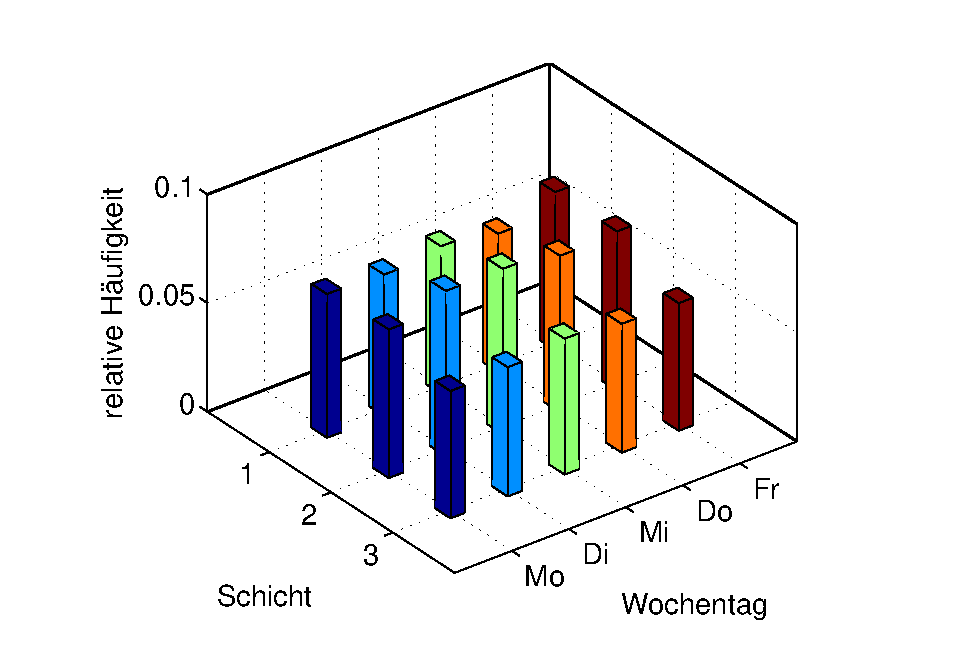
\includegraphics[width=0.5\textwidth]{Kapitel3/Bilder/image1}}
  \caption{Kausale Rechteckfunktion x(t)}
  \label{fig:LaplaceSignaleRechteck}
\end{figure}

\noindent Einsetzen der Zeitfunktion x(t) in die Definitionsgleichung führt zu

\begin{equation}\label{eq:fourfive}
X\left(s\right)=\int\limits _{0_{-} }^{\infty }x\left(t\right)\cdot e^{-s\cdot t} {\rm \; } dt=\int\limits _{0_{-} }^{\infty }\left(\sigma \left(t\right)-\sigma \left(t-t_{0} \right)\right)\cdot e^{-s\cdot t} {\rm \; } dt
\end{equation}

\noindent Die kausale Rechteckfunktion ist nur in dem Bereich von 0${}_{-}$ bis t${}_{0}$ von null verschieden. Damit muss auch die Integration nur in diesem Bereich durchgef\"{u}hrt werden. In dem Bereich ist die Funktion x(t) konstant gleich 1. Damit kann das Integral umgeformt werden zu

\begin{equation}\label{eq:foursix}
X\left(s\right)=\int\limits _{0_{-} }^{\infty }\left(\sigma \left(t\right)-\sigma \left(t-t_{0} \right)\right)\cdot e^{-s\cdot t} {\rm \; } dt=\int\limits _{0_{-} }^{t_{0} }1\cdot e^{-s\cdot t} {\rm \; } dt
\end{equation}

\noindent Mit der Stammfunktion der Exponentialfunktion

\begin{equation}\label{eq:fourseven}
\int\limits e^{a\cdot t} {\rm \; dt} =\frac{1}{a} \cdot e^{a\cdot t}
\end{equation}

\noindent und durch Einsetzen der Integrationsgrenzen ergibt sich die Laplace-Transformierte

\begin{equation}\label{eq:foureight}
X\left(s\right)=\int\limits _{0_{-} }^{t_{0} }1\cdot e^{-s\cdot t} {\rm \; } dt=\left. -\frac{1}{s} \cdot e^{-s\cdot t} \right|_{0_{-} }^{t_{0} } =-\frac{1}{s} \cdot e^{-s\cdot t_{0} } +\frac{1}{s} \cdot e^{-s\cdot 0_{-} } =\frac{1}{s} \cdot \left(1-e^{-s\cdot t_{0} } \right)
\end{equation}
\medskip

{\fontfamily{phv}\selectfont
\noindent\textbf{Impulsfunktion}}\smallskip

\noindent Als weiteres Beispiel werden die Laplace-Transformierten einer Impulsfunktion x$_{1}$(t) und einer verschobenen Impulsfunktion x$_{2}$(t) berechnet. 

\begin{equation}\label{eq:fournine}
x_{1} \left(t\right)=\delta \left(t\right)
\end{equation}

\begin{equation}\label{eq:fourten}
x_{2} \left(t\right)=\delta \left(t-t_{0} \right)
\end{equation}

\noindent Die beiden Signale sind in Bild \ref{fig:LaplaceSignaleImpuls} dargestellt.

\begin{figure}[H]
  \centerline{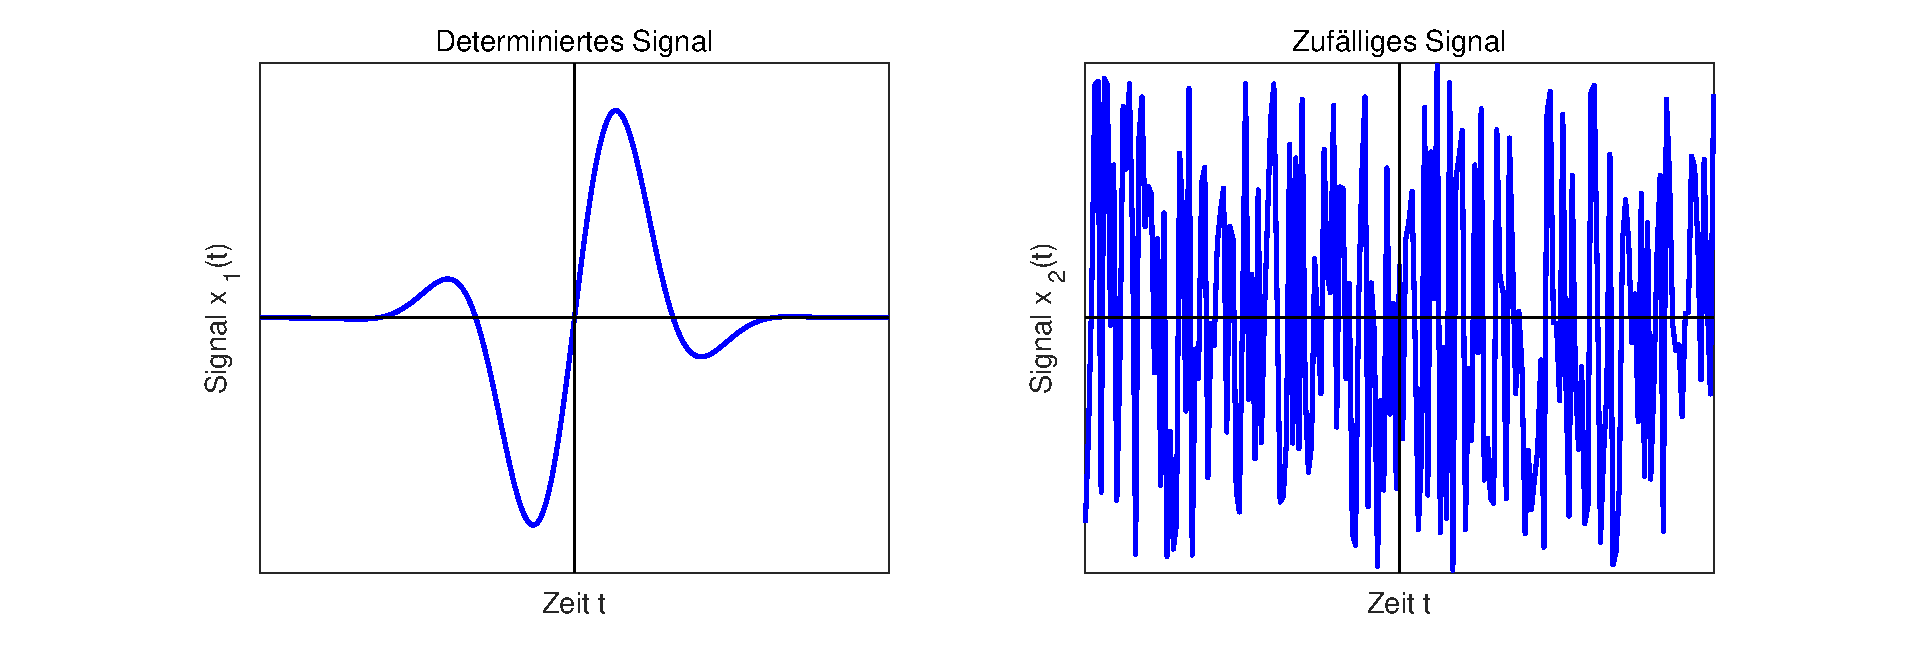
\includegraphics[width=1\textwidth]{Kapitel3/Bilder/image2}}
  \caption{Impulsfunktion x$_{1}$(t) und verschobene Impulsfunktion x$_{2}$(t)}
  \label{fig:LaplaceSignaleImpuls}
\end{figure}

\noindent Einsetzen der Impulsfunktion in die Definitionsgleichung f\"{u}hrt mit der Ausblendeigenschaft der Impulsfunktion zu

\begin{equation}\label{eq:foureleven}
X_{1} \left(s\right)=\int\limits _{0_{-} }^{\infty }\delta \left(t\right)\cdot e^{-s\cdot t} {\rm \; } dt=e^{-s\cdot 0} \cdot \int\limits _{0_{-} }^{\infty }\delta \left(t\right){\rm \; } dt=1\cdot \int\limits _{0_{-} }^{\infty }\delta \left(t\right){\rm \; } dt=1
\end{equation}

\noindent Analog ergibt sich f\"{u}r den verschobenen Impuls die Laplace-Transformierte 

\begin{equation}\label{eq:fourtwelve}
X_{2} \left(s\right)=\int _{0_{-} }^{\infty }\delta \left(t-t_{0} \right)\cdot e^{-s\cdot t} {\rm \; } dt=e^{-s\cdot t_{0} } \cdot \int _{0_{-} }^{\infty }\delta \left(t-t_{0} \right){\rm \; } dt=e^{-s\cdot t_{0} }
\end{equation}

\noindent Die Impulsfunktion $\delta$(t) besitzt die Laplace-Transformierte X(s) = 1. Eine Verschiebung des Impulses um t$_{0}$ nach rechts führt zu der Laplace-Transformierten e$^{-s\cdot t_{0}}$. In Abschnitt 4.2 wird sich zeigen, dass eine Verschiebung der Zeitfunktion um t$_{0}$ nach rechts immer zu einer Multiplikation mit dem Faktor e$^{-s\cdot t_{0}}$ führt.\bigskip

{\fontfamily{phv}\selectfont
\noindent\textbf{Sprungfunktion}}\smallskip

\noindent Die Sprungfunktion $\sigma$(t) springt zum Zeitpunkt t = 0 von null auf den Wert eins. Sie ist in Bild \ref{fig:LaplaceSignaleSprung} dargestellt.

\begin{figure}[H]
  \centerline{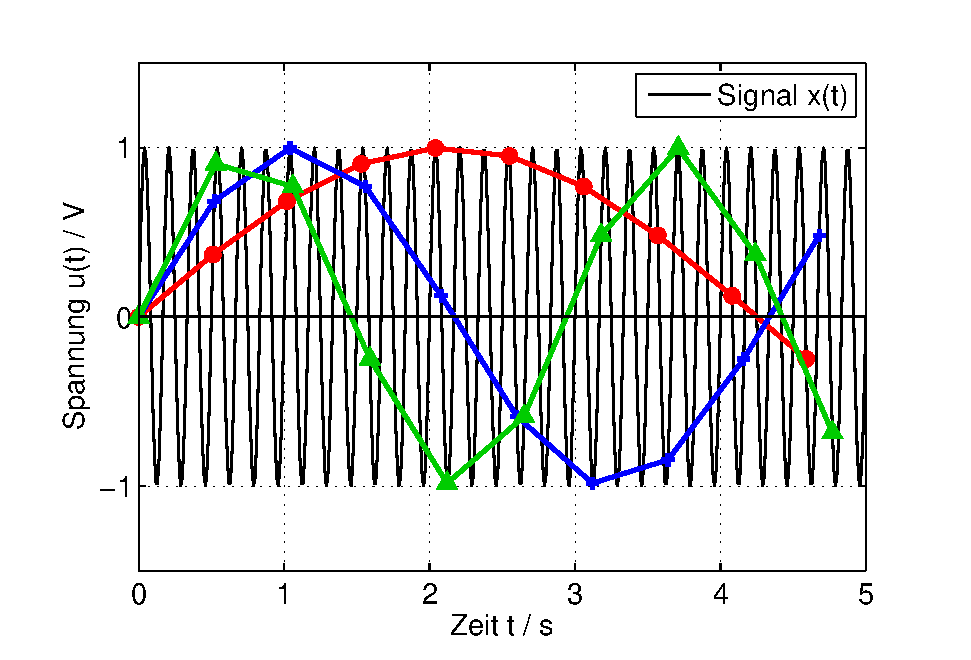
\includegraphics[width=0.5\textwidth]{Kapitel3/Bilder/image3}}
  \caption{Sprungfunktion $\sigma$}
  \label{fig:LaplaceSignaleSprung}
\end{figure}

\begin{equation}\label{eq:fourthirteen}
X\left(s\right)=\int\limits _{0_{-} }^{\infty }\sigma \left(t\right)\cdot e^{-s\cdot t} \;dt=\int\limits _{0_{-} }^{\infty }1\cdot e^{-s\cdot t} \;dt=\int\limits _{0_{-} }^{\infty }e^{-s\cdot t}\; dt
\end{equation}

\noindent Da die Sprungfunktion zeitlich nicht begrenzt ist, weist das Integral einen unendlich langen Integrationsbereich auf. Derartige Integrale werden uneigentliche Integrale genannt. Bilden der Stammfunktion und Einsetzen der Integrationsgrenzen führen zu dem Ausdruck

\begin{equation}\label{eq:fourfourteen}
X\left(s\right)=\left. -\frac{1}{s} \cdot e^{-s\cdot t} \right|_{0_{-} }^{\infty } =-\lim \limits_{t\to \infty } \frac{1}{s} \cdot e^{-s\cdot t} +\frac{1}{s} \cdot e^{-s\cdot 0_{-} } =\frac{1}{s} \cdot \left(1-\lim \limits_{t\to \infty } e^{-s\cdot t} \right)
\end{equation}

\noindent Dabei ist die Zahl s eine komplexe Zahl s = $\delta$ + j$\cdot\omega$. Der Grenzwert existiert nur, wenn der Realteil $\delta$ der komplexen Zahl s positiv ist. In diesem Fall gilt

\begin{equation}\label{eq:fourfifteen}
X\left(s\right)=\frac{1}{s} \cdot \left(1-\lim\limits_{t\to \infty} e^{-s\cdot t} \right)=\frac{1}{s} \cdot \left(1-\lim\limits_{t\to \infty } e^{-\left(\delta +j\cdot \omega \right)\cdot t} \right)=\frac{1}{s} \cdot \left(1-\lim\limits_{t\to \infty } e^{-\delta \cdot t} \cdot e^{-j\cdot \omega \cdot t} \right)=\frac{1}{s} \cdot \left(1-0\right)=\frac{1}{s}
\end{equation}

\noindent Die Sprungfunktion x(t) = $\sigma$(t) hat demnach für den Bereich der s-Ebene mit $\delta$ $\mathrm{>}$ 0 die Laplace-Transformierte X(s) = 1/s. In dem Bereich der s-Ebene mit $\delta$ $\leq$ 0 besitzt die Sprungfunktion keine Laplace-Transformierte, da das Laplace-Integral nicht konvergiert.\medskip

\noindent Zu der Laplace-Transformierten muss demnach immer ein Konvergenzbereich angegeben werden. In den beiden ersten Beispielen ist der Konvergenzbereich unendlich gro{\ss}. Bei der Sprungfunktion liegt der Konvergenzbereich in der positiven Halbebene. Auf die Frage der Konvergenz des Laplace-Integrals wird in Abschnitt 4.1.3 genauer eingegangen.\bigskip

{\fontfamily{phv}\selectfont
\noindent\textbf{Konstanten und kausale Konstanten}}\smallskip

\noindent Die Laplace-Transformierte einer Konstanten x(t) = k ergibt sich analog zu der Berechnung der Laplace-Transformierten der Sprungfunktion zu

\begin{equation}\label{eq:foursixteen}
X\left(s\right)=\int _{0_{-} }^{\infty }k\cdot e^{-s\cdot t} \; dt=k\cdot \int _{0_{-} }^{\infty }e^{-s\cdot t} \; dt=\frac{k}{s}
\end{equation}

\noindent Die Laplace-Transformierten einer Konstante k und einer mit dem Faktor k multiplizierten Sprungfunktion k$\cdot\sigma$(t) unterscheiden sich weder im Ergebnis noch im Konvergenzbereich. Ursache ist die einseitige Laplace-Transformation mit der Definitionsgleichung

\begin{equation}\label{eq:fourseventeen}
X\left(s\right)=\int _{0_{-} }^{\infty }x\left(t\right)\cdot e^{-s\cdot t} \; dt
\end{equation}

\noindent Die Integration beginnt zum Zeitpunkt t = 0$_{-}$, sodass das Verhalten der Funktion für t $\mathrm{<}$ 0 unberücksichtigt bleibt. Da sich Konstanten und Sprungfunktionen aber nur in diesem Bereich unterscheiden, ist ihre Laplace-Transformierte identisch. Bild \ref{fig:LaplaceSignaleKausaleKonstant} verdeutlicht diesen Zusammenhang grafisch.

\begin{figure}[H]
  \centerline{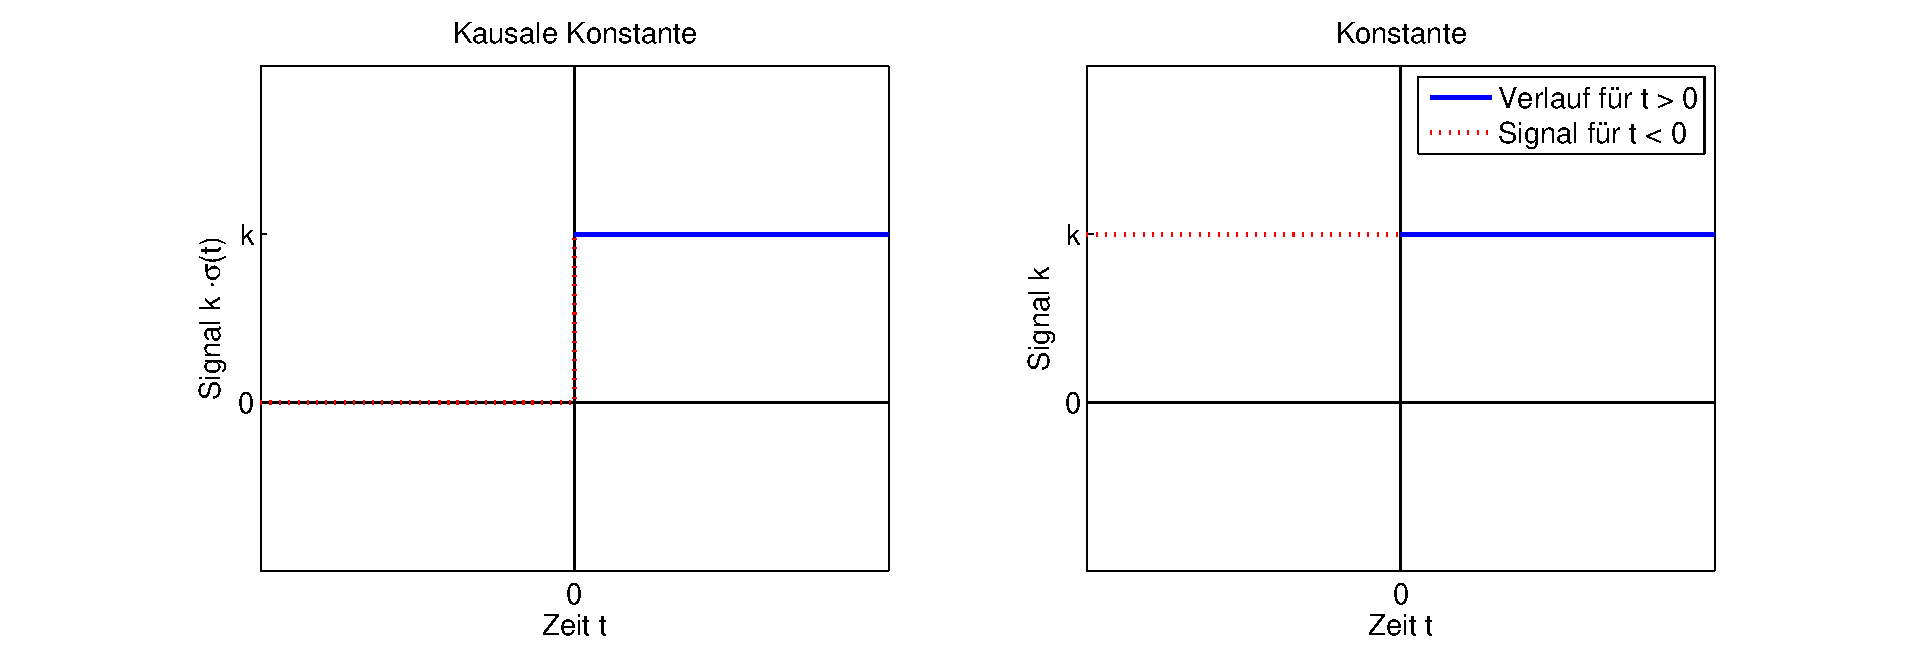
\includegraphics[width=1\textwidth]{Kapitel3/Bilder/image4}}
  \caption{Grafischer Vergleich von kausaler Konstante k$\sigma$(t) und Konstante k}
  \label{fig:LaplaceSignaleKausaleKonstant}
\end{figure}

\noindent Konstanten werden im Zusammenhang mit der Laplace-Transformation auch als kausale Konstanten bezeichnet, also als Konstanten, die erst für t $\geq$ 0 von null verschieden sind.\bigskip

{\fontfamily{phv}\selectfont
\noindent\textbf{Kausale Exponentialfunktion}}\smallskip

\noindent Die kausale Exponentialfunktion ist für t $\mathrm{<}$ 0 null. Zum Zeitpunkt t = 0 springt sie auf den Wert eins. Je nach Koeffizienten $\delta$ steigt die Exponentialfunktion an, bleibt konstant oder fällt ab. 

\begin{equation}\label{eq:foureighteen}
x\left(t\right)=e^{\delta \cdot t} \cdot \sigma \left(t\right) 
\end{equation}

\noindent Bild \ref{fig:KomplexExponentialfunktion} verdeutlicht die Abhängigkeit des Signalverlaufs von dem Koeffizienten $\delta$.

\begin{figure}[H]
  \centerline{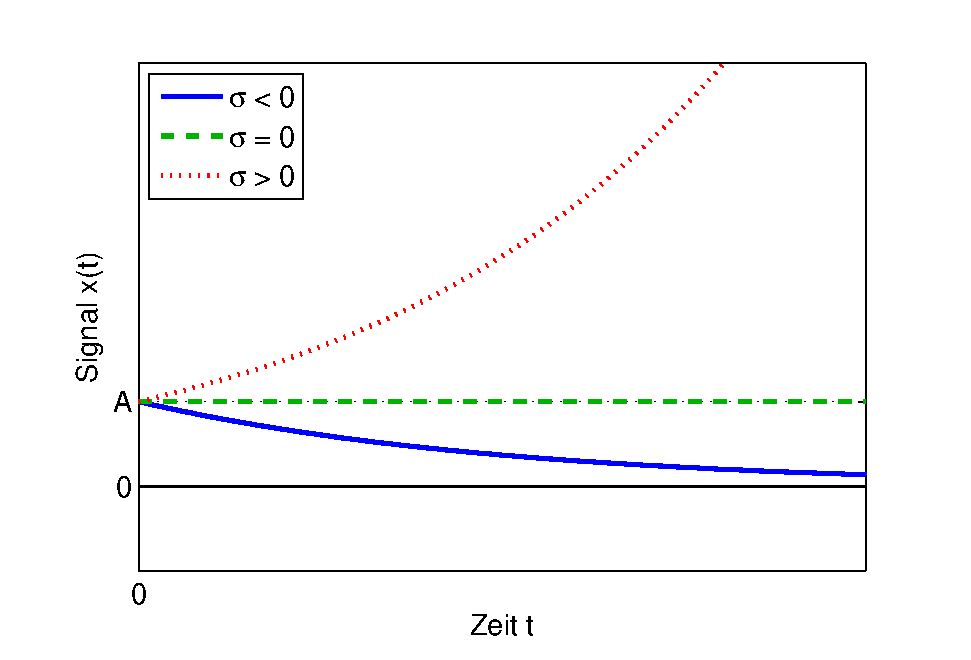
\includegraphics[width=0.5\textwidth]{Kapitel3/Bilder/image5}}
  \caption{Kausale Exponentialfunktion mit unterschiedlichen Koeffizienten $\sigma$ = - 1, 0 und 1}
  \label{fig:LaplaceSignaleExponentialfunktion}
\end{figure}

\noindent Wird die kausale Exponentialfunktion in die Definitionsgleichung für die Laplace-Transformation
eingesetzt, ergibt sich das Integral

\begin{equation}\label{eq:fournineteen}
X\left(s\right)=\int\limits _{0_{-} }^{\infty }e^{\delta \cdot t} \cdot \sigma \left(t\right)\cdot e^{-s\cdot t}\; dt=\int\limits _{0_{-} }^{\infty }e^{\left(\delta -s\right)\cdot t} \;dt 
\end{equation}

\noindent Wieder handelt es sich um ein uneigentliches Integral. Dasselbe Vorgehen wie bei der Sprungfunktion führt zu 

\begin{equation}\label{eq:fourtwenty}
X\left(s\right)=\left. \frac{1}{\delta -s} \cdot e^{\left(\delta -s\right)\cdot t} \right|_{0_{-} }^{\infty } =\lim \limits_{t\to \infty }  \frac{1}{\delta -s} \cdot e^{\left(\delta -s\right)\cdot t} -\frac{1}{\delta -s} \cdot e^{\left(\delta -s\right)\cdot 0_{-} } =\frac{1}{s-\delta } \cdot \left(1-\lim \limits_{t\to \infty } e^{-\left(s-\delta \right)\cdot t} \right)
\end{equation}

\noindent Der Grenzwert existiert nur, wenn Re(s - $\delta$) $\mathrm{>}$ 0 ist. In dem Fall gilt

\begin{equation}\label{eq:fourtwentyone}
X\left(s\right)=\frac{1}{s-\delta } \cdot \left(1-\lim\limits_{t\to \infty } e^{-\left(s-\delta \right)\cdot t} \right)=\frac{1}{s-\delta } 
\end{equation}

\noindent Die kausale Exponentialfunktion hat demnach f\"{u}r den Bereich der s-Ebene mit Re(s - $\delta$) $\mathrm{>}$ 0 die Laplace-Transformierte X(s) = 1/(s - $\delta$). In dem \"{u}brigen Bereich der s-Ebene besitzt die kausale Exponentialfunktion keine Laplace-Transformierte, da das Laplace-Integral nicht konvergiert. 

\subsubsection{Existenz der Laplace-Transformation}

\noindent Die Laplace-Transformation beruht auf der Auswertung des Laplace-Integrals.

\begin{equation}\label{eq:fourtwentytwo}
X\left(s\right)=\int\limits _{0_{-} }^{\infty }x\left(t\right)\cdot e^{-s\cdot t} \; dt
\end{equation}

\noindent Es ist ein uneigentliches Integral, das nur definiert ist, wenn das Integral konvergiert. Diese Bedingung ist erfüllt, wenn x(t) stückweise stetig ist und wenn {\textbar}x(t){\textbar} für t $\rightarrow$ $\infty$ nicht schneller als eine Exponentialfunktion wächst. In dem Fall kann die Funktion x(t) abgeschätzt werden mit 

\begin{equation}\label{eq:fourtwentythree}
\left|x\left(t\right)\right|\le k\cdot e^{\delta \cdot t}
\end{equation}

\noindent Für Re(s) $\mathrm{>}$ $\delta$ ist das zugehörige Laplace-Integral absolut konvergent, und die Laplace-Transformierte existiert. Dies kann durch Einsetzen in das Laplace-Integral verdeutlicht werden. Mit 

\begin{equation}\label{eq:fourtwentyfour}
x\left(t\right)=e^{\delta \cdot t} \cdot \sigma \left(t\right)
\end{equation}

\noindent ergibt sich

\begin{equation}\label{eq:fourtwentyfive}
X\left(s\right)=\int\limits _{0_{-} }^{\infty }e^{\delta \cdot t} \cdot \sigma \left(t\right)\cdot e^{-s\cdot t} \; dt= \int\limits _{0_{-} }^{\infty }e^{\left(\delta -s\right)\cdot t} \; dt= \left. \frac{1}{\delta -s} \cdot e^{-\left(s-\delta \right)\cdot t} \right|_{0_{-} }^{\infty } =\lim \limits_{t\to \infty } \frac{1}{\delta -s} \cdot e^{-\left(s-\delta \right)\cdot t} -\frac{1}{\delta -s}
\end{equation}

\noindent Für Re(s - $\delta$) $\mathrm{<}$ 0 strebt die Exponentialfunktion gegen unendlich, das Integral ist demnach nicht konvergent, die Laplace-Transformierte existiert f\"{u}r diesen Bereich der s-Ebene nicht. F\"{u}r Re(s - $\delta$) $\mathrm{>}$ 0 strebt die Exponentialfunktion für t $\rightarrow$ $\infty$ gegen null. Das Integral ist konvergent, und die Laplace-Transformierte existiert. Bild \ref{fig:KonvergenzBereich} zeigt den Konvergenzbereich des Laplace-Integrals in der komplexen Ebene.

\begin{figure}[H]
  \centerline{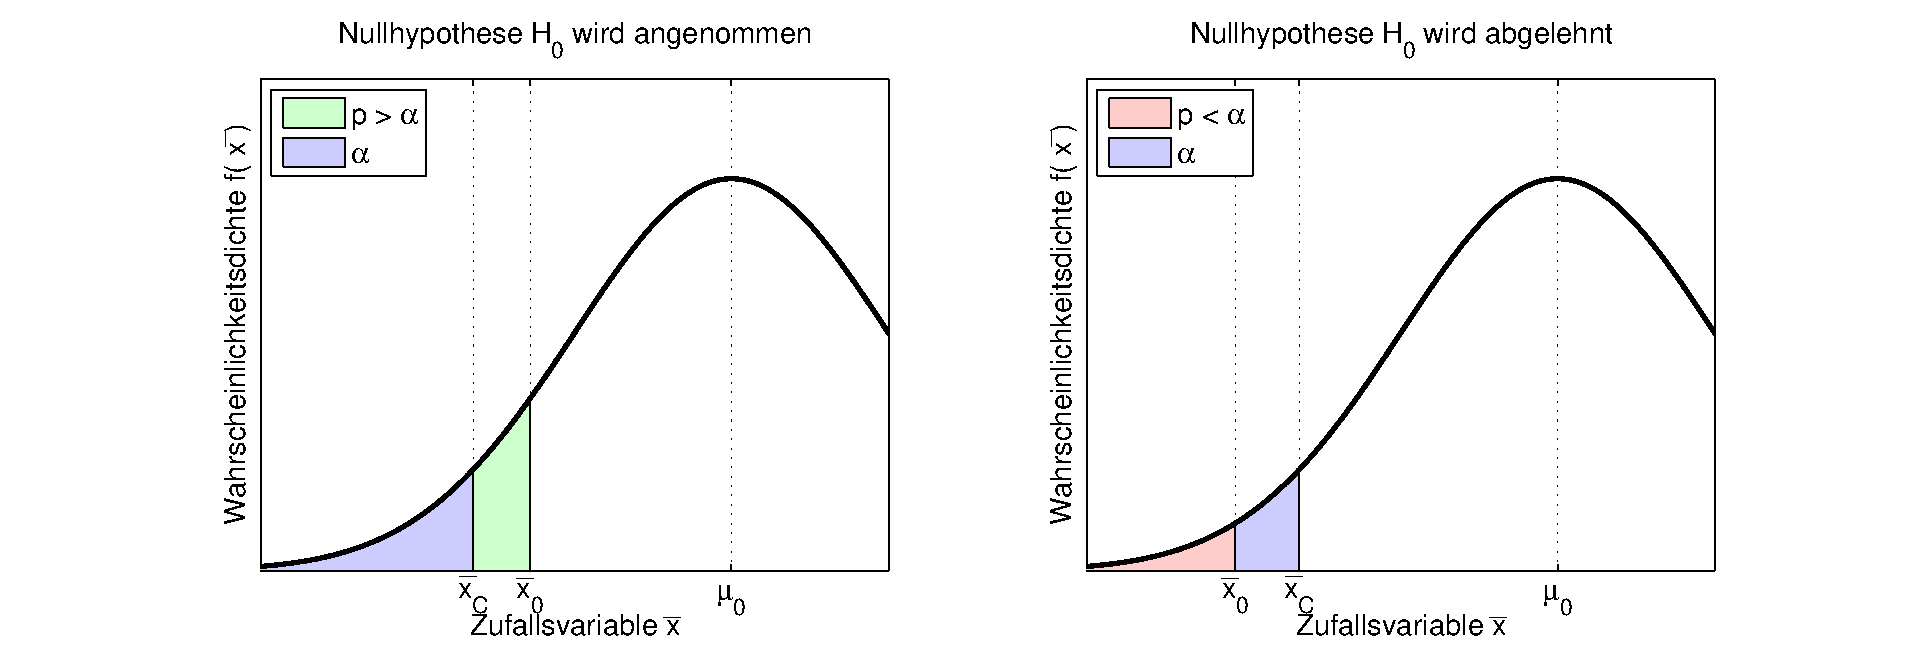
\includegraphics[width=0.4\textwidth]{Kapitel3/Bilder/image6}}
  \caption{Konvergenzbereich für Re(s -$\sigma$) $\mathrm{>}$ 0}
  \label{fig:KonvergenzBereich}
\end{figure}

\noindent Für den grau hinterlegten Bereich der s-Ebene ist das Laplace-Integral konvergent. Allgemein existiert eine Laplace-Transformierte X(s) einer Funktion x(t) also, wenn {\textbar}x(t){\textbar} für t $\rightarrow$ $\infty$ nicht schneller wächst als eine Exponentialfunktion. In den systemtheoretisch interessanten Fällen kann von der Konvergenz des Laplace-Integrals zumindest in einem Teil der s-Ebene ausgegangen werden. Der Konvergenzbereich der Laplace-Transformation ist deshalb für die Berechnung technisch interessanter Fälle von untergeordneter Bedeutung.\medskip

\noindent Bei der sogenannten Fourier-Transformation ist der Konvergenzbereich der Laplace-Transformation wieder wichtig. Es wird sich zeigen, dass sich die Fourier-Transformierte direkt aus der Laplace-Transformierten ergibt, wenn die imagin\"{a}re Achse s = j$\cdot\omega$ im Konvergenzbereich der Laplace-Transformierten liegt.

\clearpage 

\subsubsection{Pollage und kausale Exponentialfunktion}

\noindent Im Abschnitt 4.1.2 wird die Laplace-Transformierte der kausalen Exponentialfunktion

\begin{equation}\label{eq:fourtwentysix}
x\left(t\right)=e^{\lambda \cdot t} \cdot \sigma \left(t\right)
\end{equation}

\noindent berechnet zu

\begin{equation}\label{eq:fourtwentyseven}
X\left(s\right)=\frac{1}{s-\lambda }
\end{equation}

\noindent Aus Gleichung \eqref{eq:fourtwentyseven} kann der zu der Exponentialfunktion zugehörige Pol in der komplexen s-Ebene abgelesen werden.

\begin{equation}\label{eq:fourtwentyeight}
s=\lambda 
\end{equation}

\noindent Die Lage des Poles beziehungsweise der Pole in der s-Ebene kann damit einem Signalverhalten zugeordnet werden, das in Tabelle\ref{tab:fourone} skizziert ist.\medskip

\noindent Kosinusfunktionen mit exponentiell abklingender Amplitude k\"{o}nnen nach den Darstellungen in Abschnitt 2.4.2 als Summe zweier Exponentialfunktionen mit jeweils konjugiert komplexen Koeffizienten $\lambda$ dargestellt werden. 


\begin{equation}\label{eq:fourtwentynine}
\begin{split}
x\left(t\right) & = A\cdot e^{\delta _{0} \cdot t} \cdot \cos \left(\omega _{0} \cdot t\right)\cdot \sigma \left(t\right)=\frac{1}{2} \cdot A\cdot e^{\delta _{0} \cdot t} \cdot \left(e^{j\cdot \omega _{0} \cdot t} +e^{-j\cdot \omega _{0} \cdot t} \right)\cdot \sigma \left(t\right) \\ 
& = \frac{1}{2} \cdot A\cdot \left(e^{\left(\delta _{0} +j\cdot \omega _{0} \right)\cdot t} +e^{\left(\delta _{0} -j\cdot \omega _{0} \right)\cdot t} \right)\cdot \sigma \left(t\right)
\end{split}
\end{equation}

\noindent Jede Exponentialfunktion führt zu einem Pol in der komplexen Ebene, sodass in diesem Fall konjugiert komplexe Polpaare auftreten. Der Realteil $\delta{0}$ der Pole beschreibt das Verhalten der Amplitude, die Imagin\"{a}rteil $\omega _{0}$ repräsentiert die Kreisfrequenz, mit der das Signal schwingt. Die Lage der konjugiert komplexen Polpaare und das entsprechende Signalverhalten sind ebenfalls in Tabelle \ref{tab:fourone} skizziert.\medskip

\noindent Der Zusammenhang von Pollage der Laplace-Transformierten X(s) und dem Einschwingverhalten der zugehörigen Zeitfunktion x(t) ist Grundlage für die Interpretation linearer, zeitinvarianter Systeme im Laplace-Bereich.

\InsertBoxL{0}{\includegraphics[scale=0.5]{code}} 
\textcolor{white}{.}\newline
\noindent Im Online-Portal \textit{Systemtheorie Online} verdeutlicht die Applikation \textit{Komplexe Exponentialfunktion} den Zusammenhang zwischen der Lage des Wertes $\lambda = \delta + j.\omega{}_{0}$ in der komplexen Ebene und dem Verhalten der Schwingung.\newline

\clearpage

\begin{table}[ht]
\setlength{\arrayrulewidth}{.1em}
\caption{Zusammenhang zwischen Pollage der Laplace-Transformierten X(s) in der komplexen Ebene und
Signalverlauf x(t)}
\setlength{\fboxsep}{0pt}%
\colorbox{lightgray}{%
\arrayrulecolor{white}%
\begin{tabular}{| c | c |}
\hline
\parbox[c][0.28in][c]{3.2in}{\smallskip\centering\textbf{\fontfamily{phv}\selectfont{Pollage X(s)}}} & \parbox[c][0.28in][c]{3.2in}{\smallskip\centering\textbf{\fontfamily{phv}\selectfont{Signalverlauf x(t)}}}\\ \hline

\parbox[c][1.6in][c]{3.2in}{\centerline{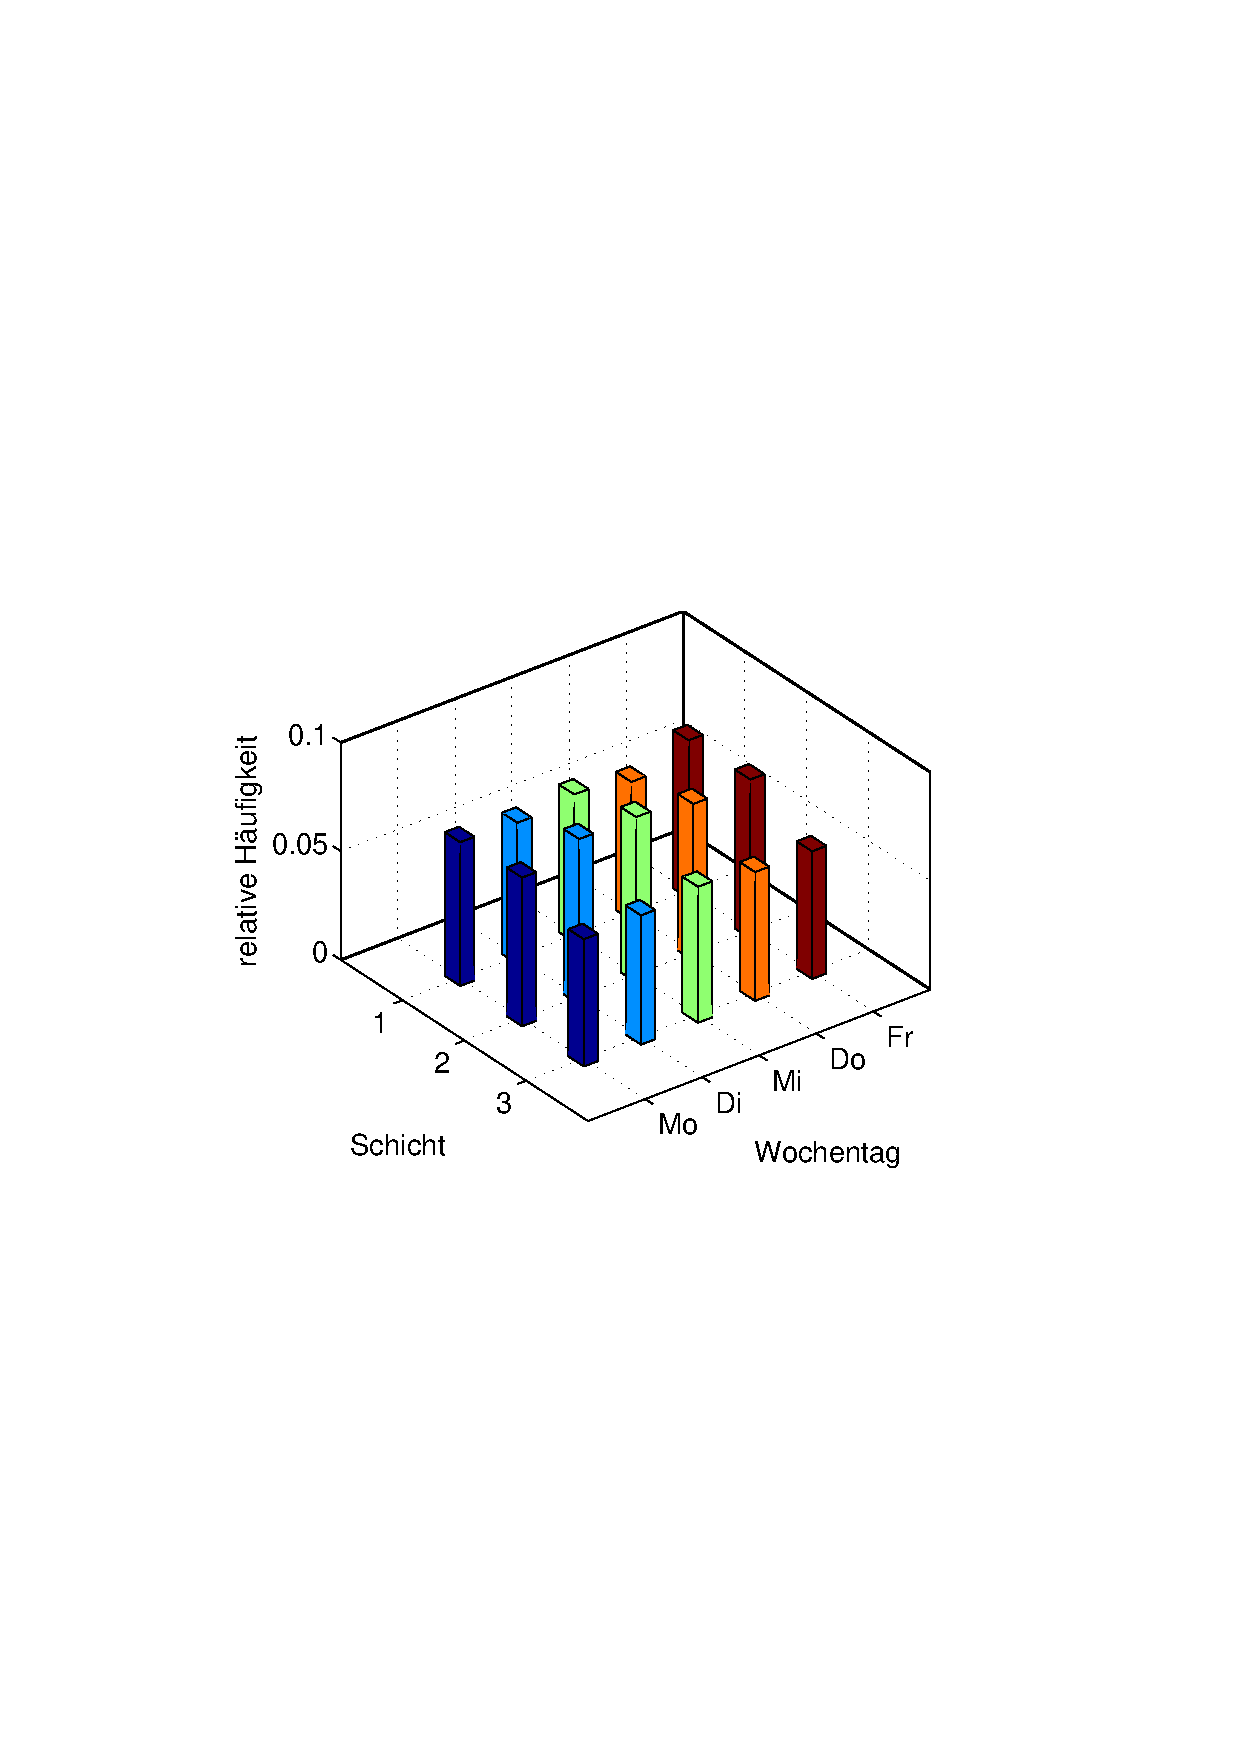
\includegraphics[width=0.3\textwidth]{Kapitel3/Table/image1.png}}} & \parbox[c][1.6in][c]{3.2in}{\centerline{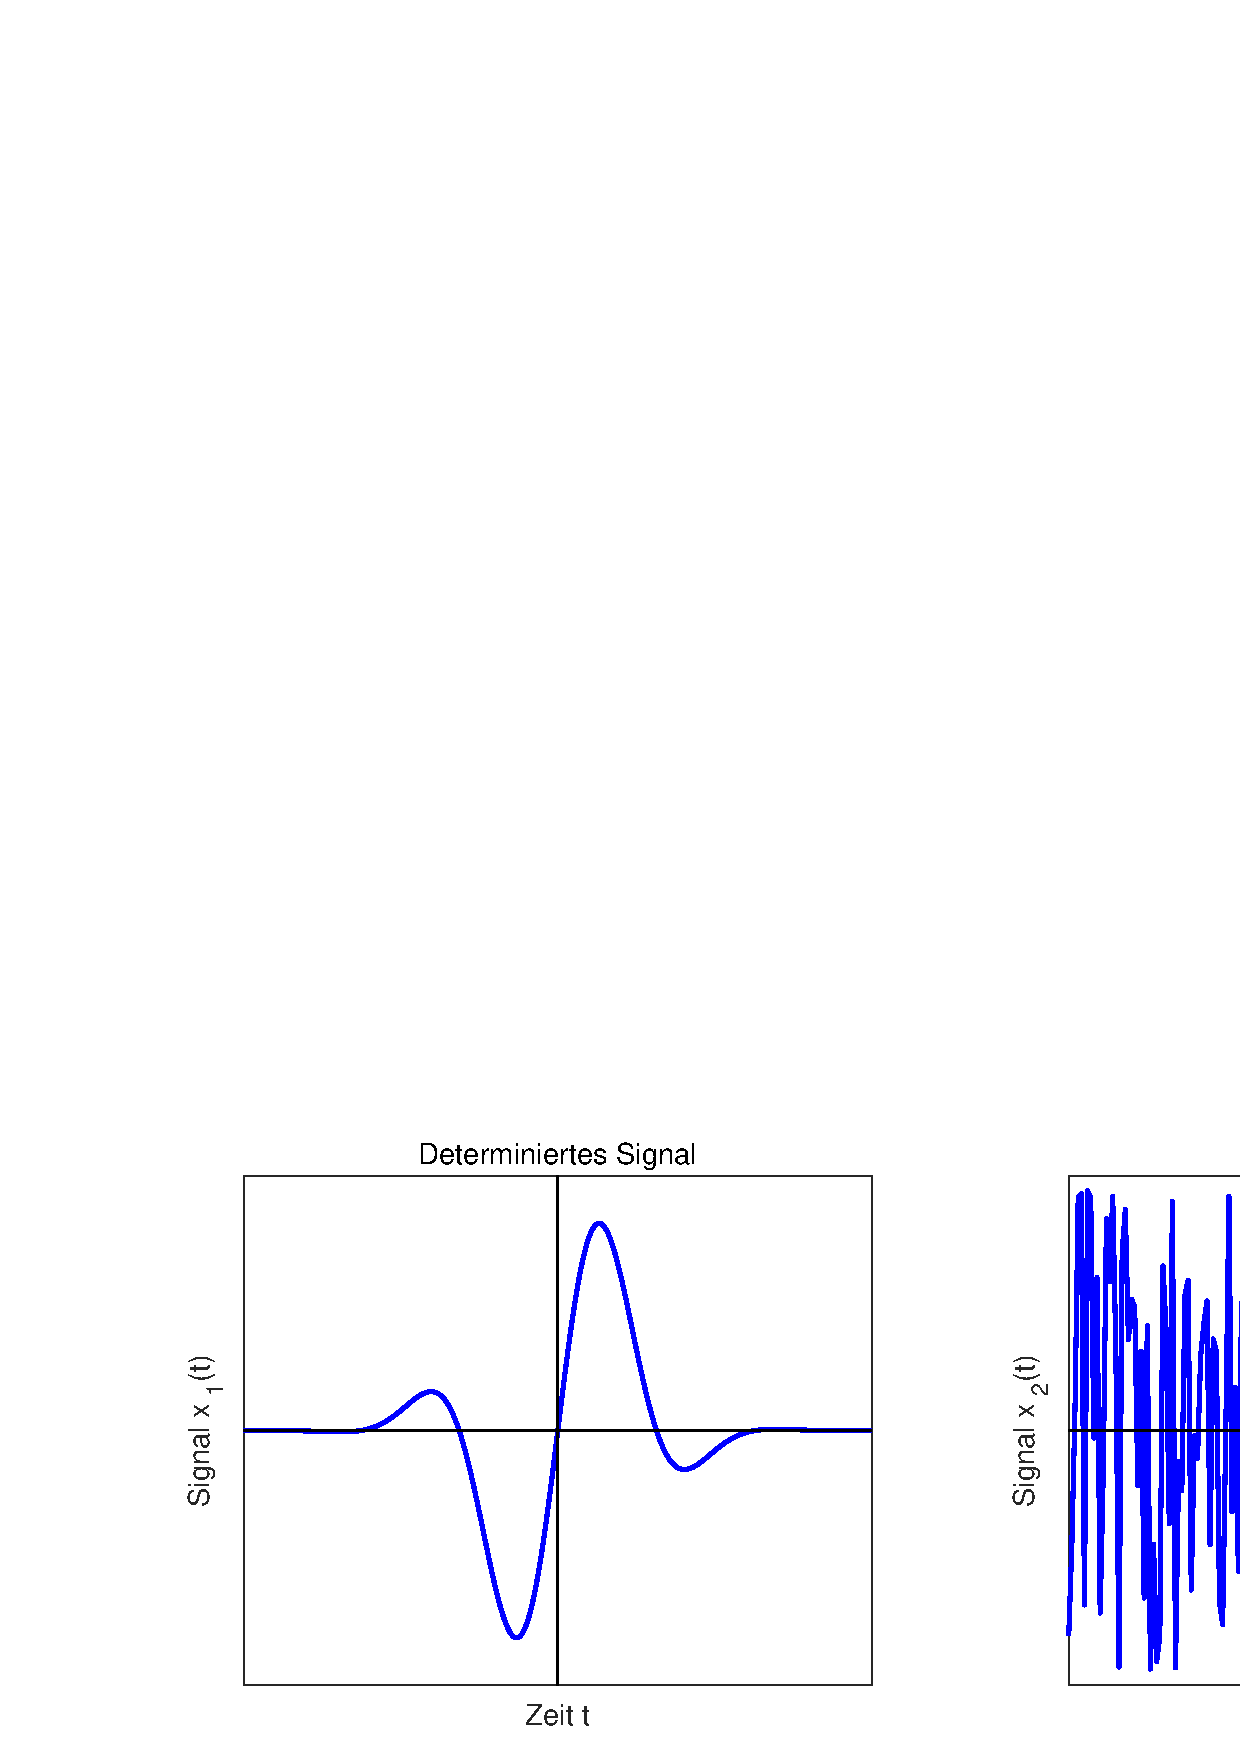
\includegraphics[width=0.3\textwidth]{Kapitel3/Table/image2.png}}}\\ \hline

\parbox[c][1.6in][c]{3.2in}{\centerline{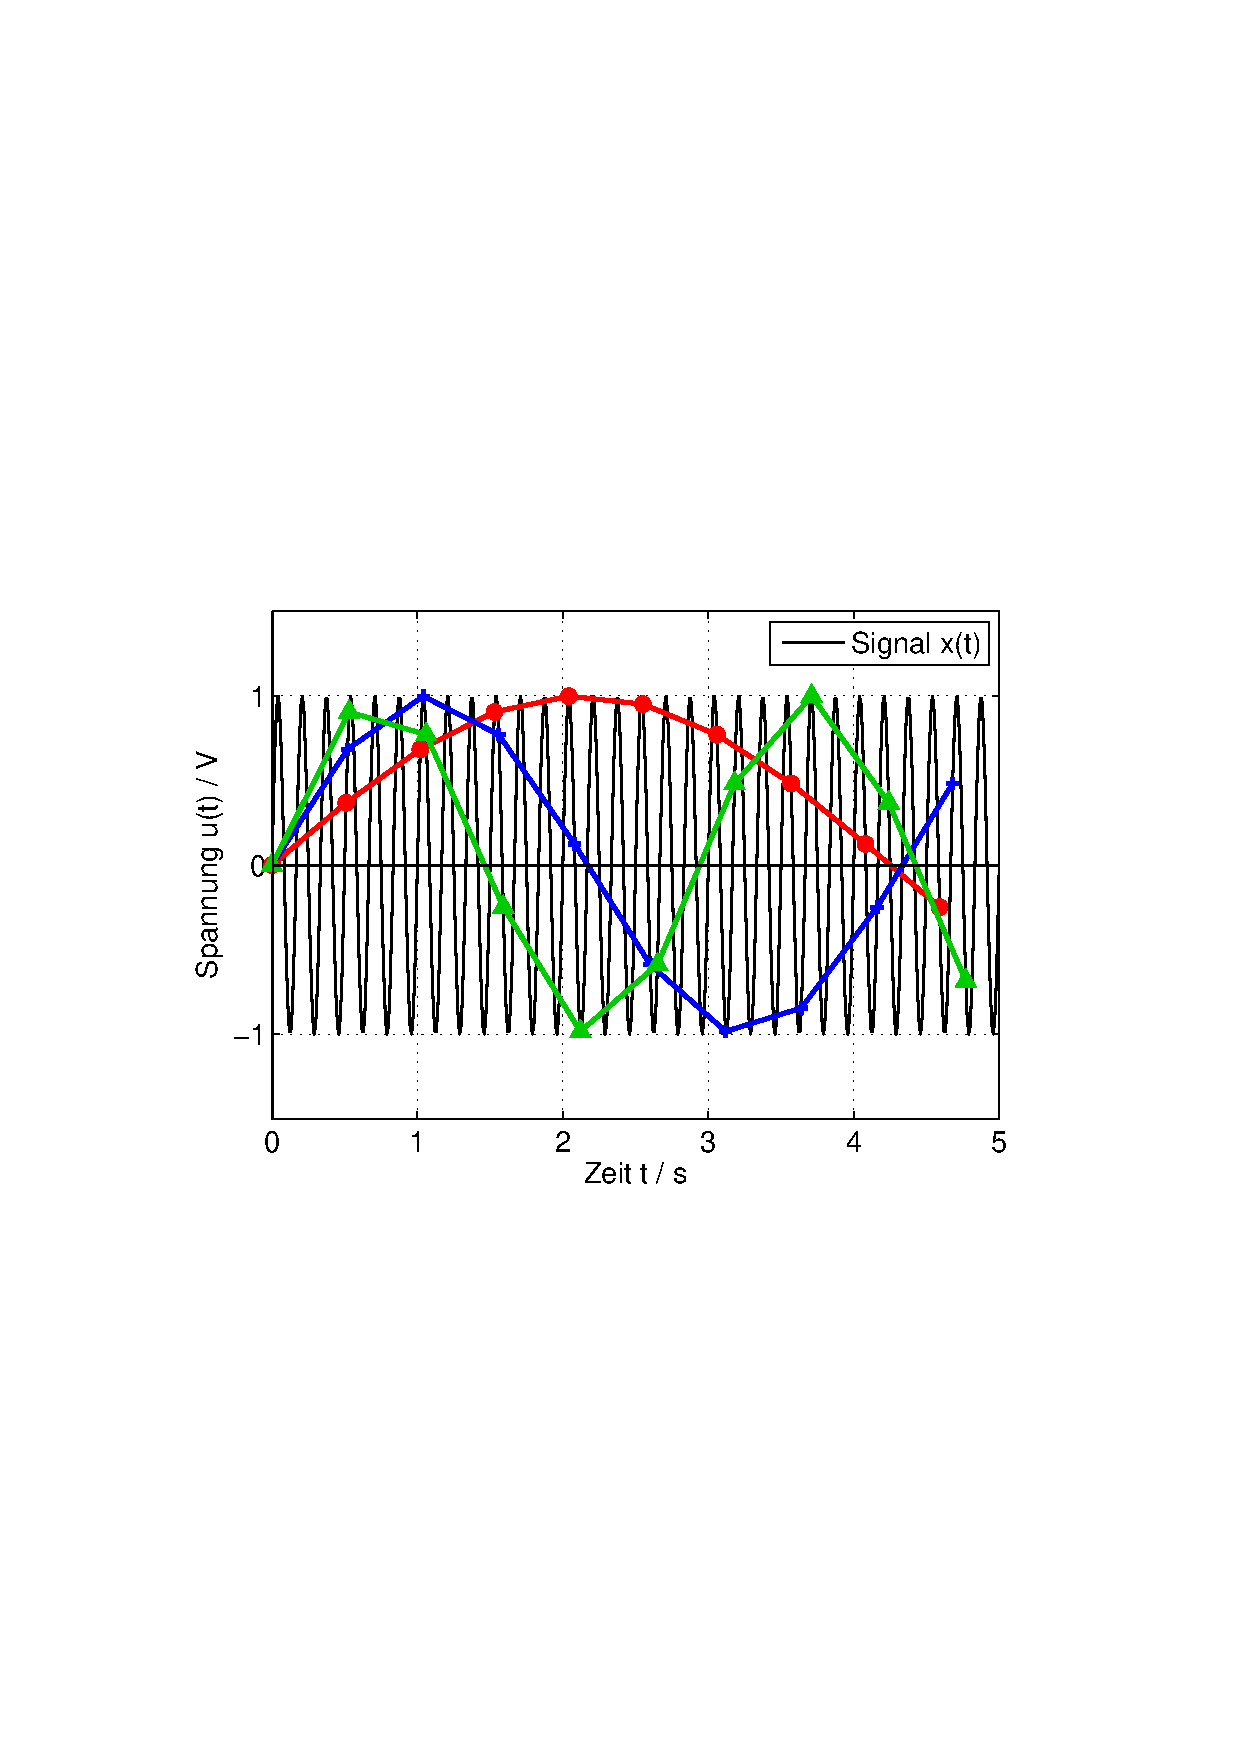
\includegraphics[width=0.3\textwidth]{Kapitel3/Table/image3.png}}} & \parbox[c][1.6in][c]{3.2in}{\centerline{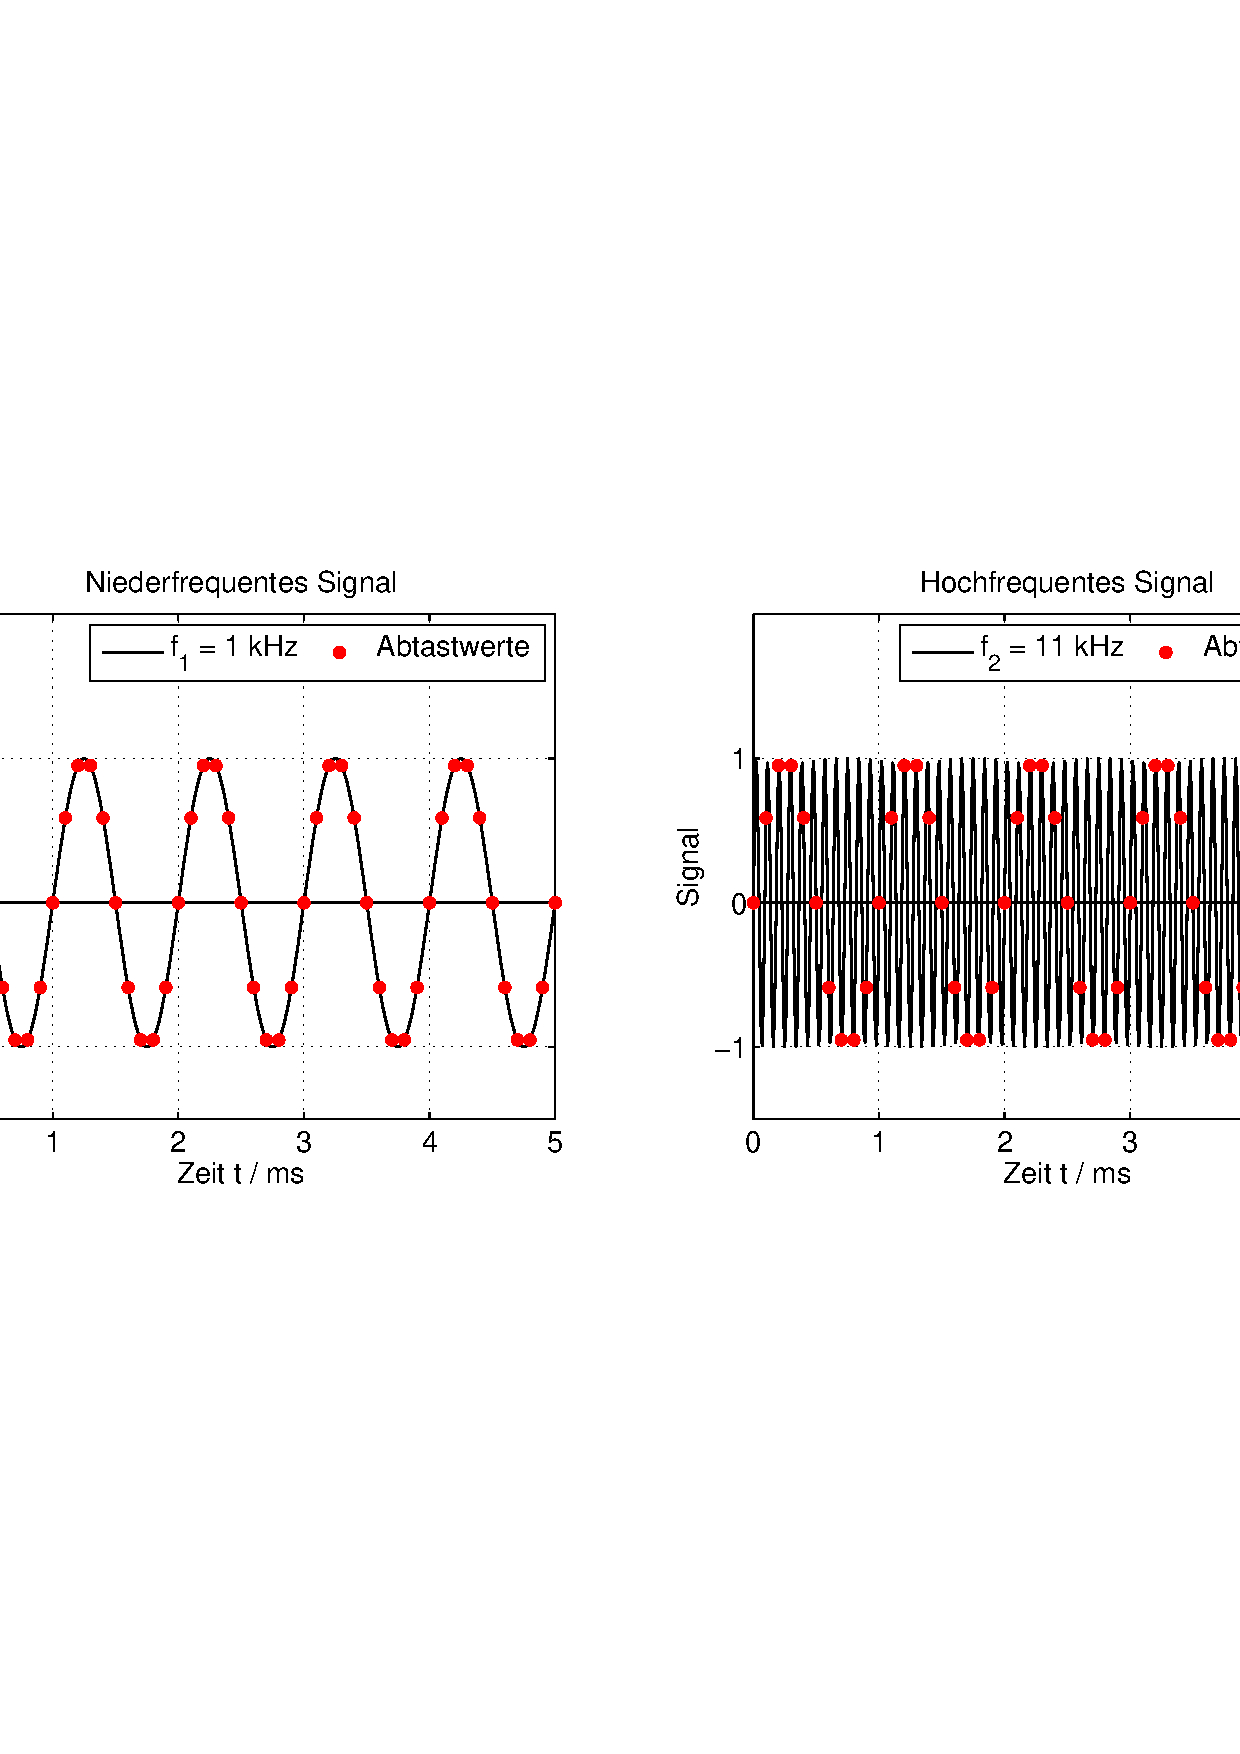
\includegraphics[width=0.3\textwidth]{Kapitel3/Table/image4.png}}}\\ \hline

\parbox[c][1.6in][c]{3.2in}{\centerline{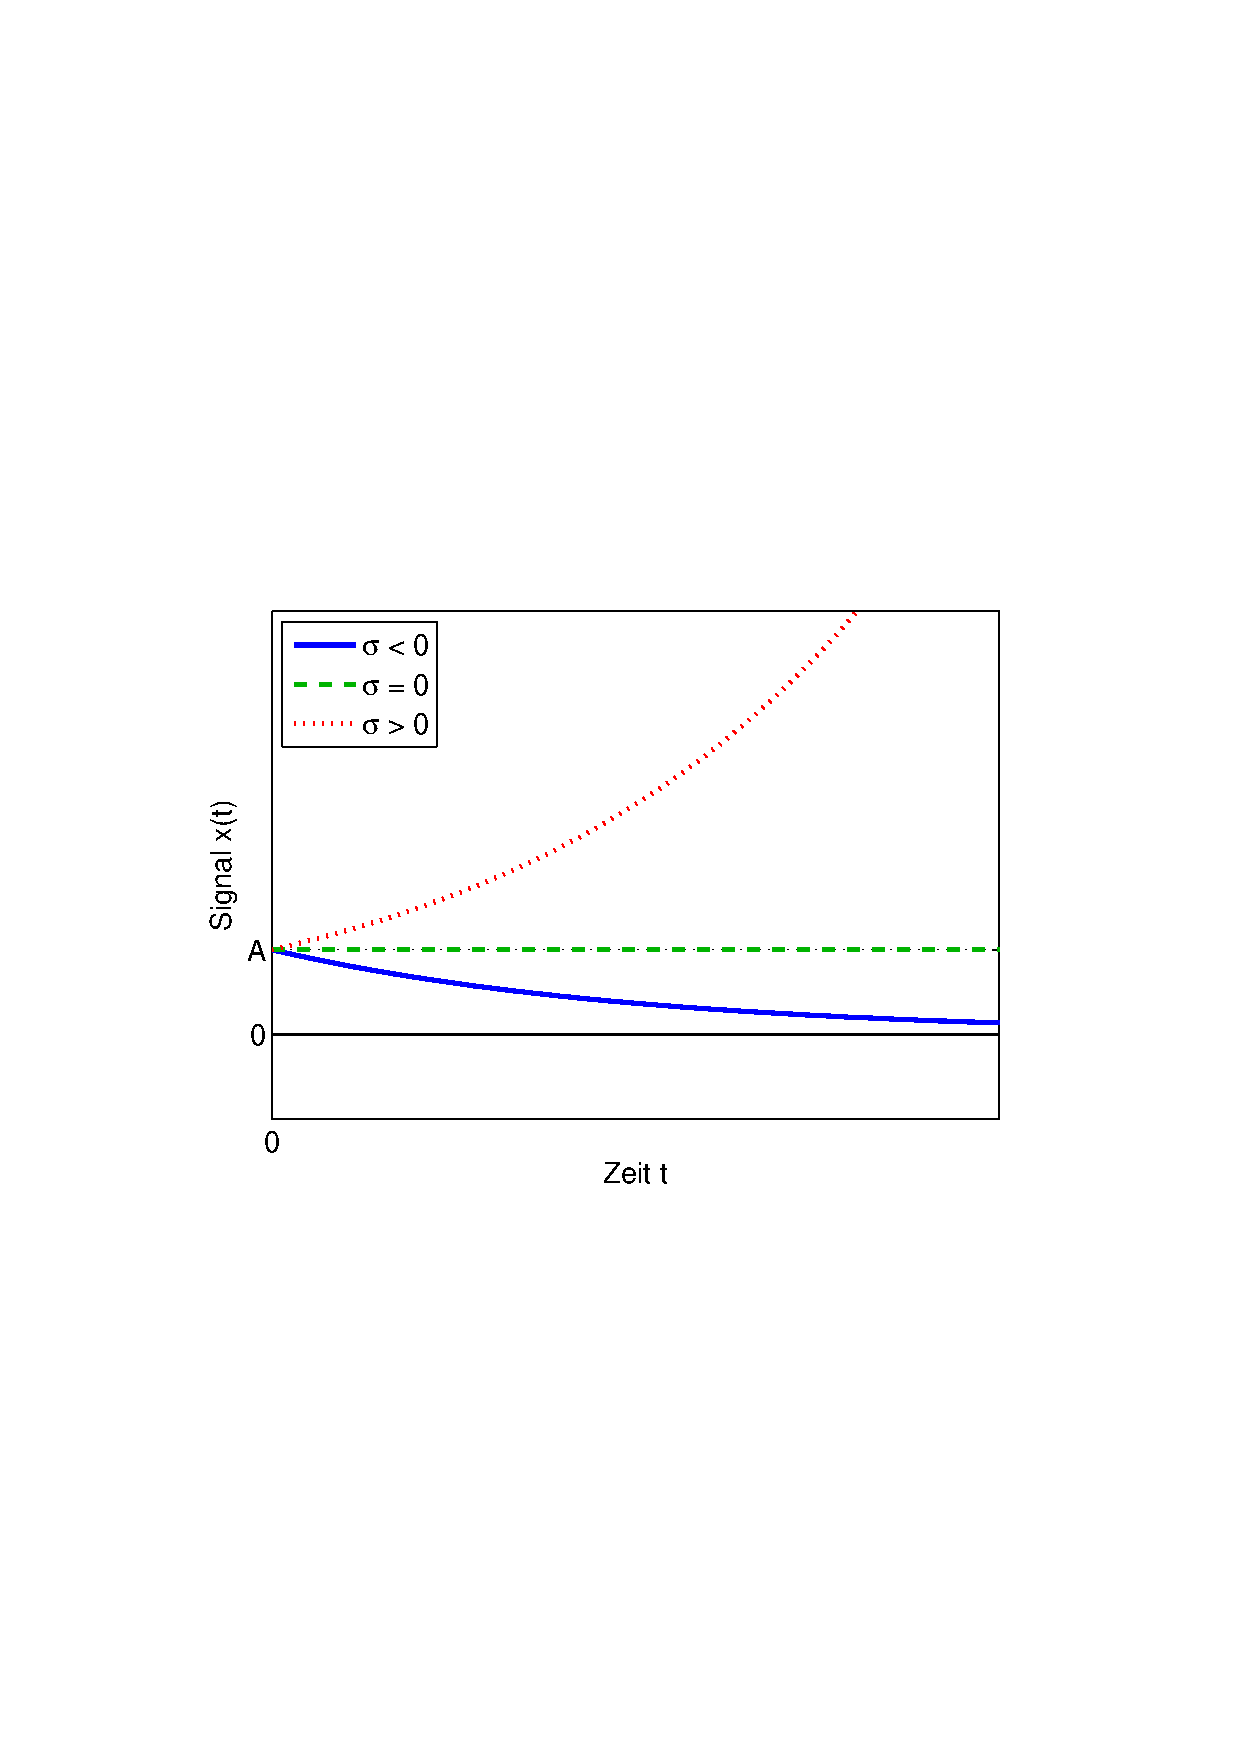
\includegraphics[width=0.3\textwidth]{Kapitel3/Table/image5.png}}} & \parbox[c][1.6in][c]{3.2in}{\centerline{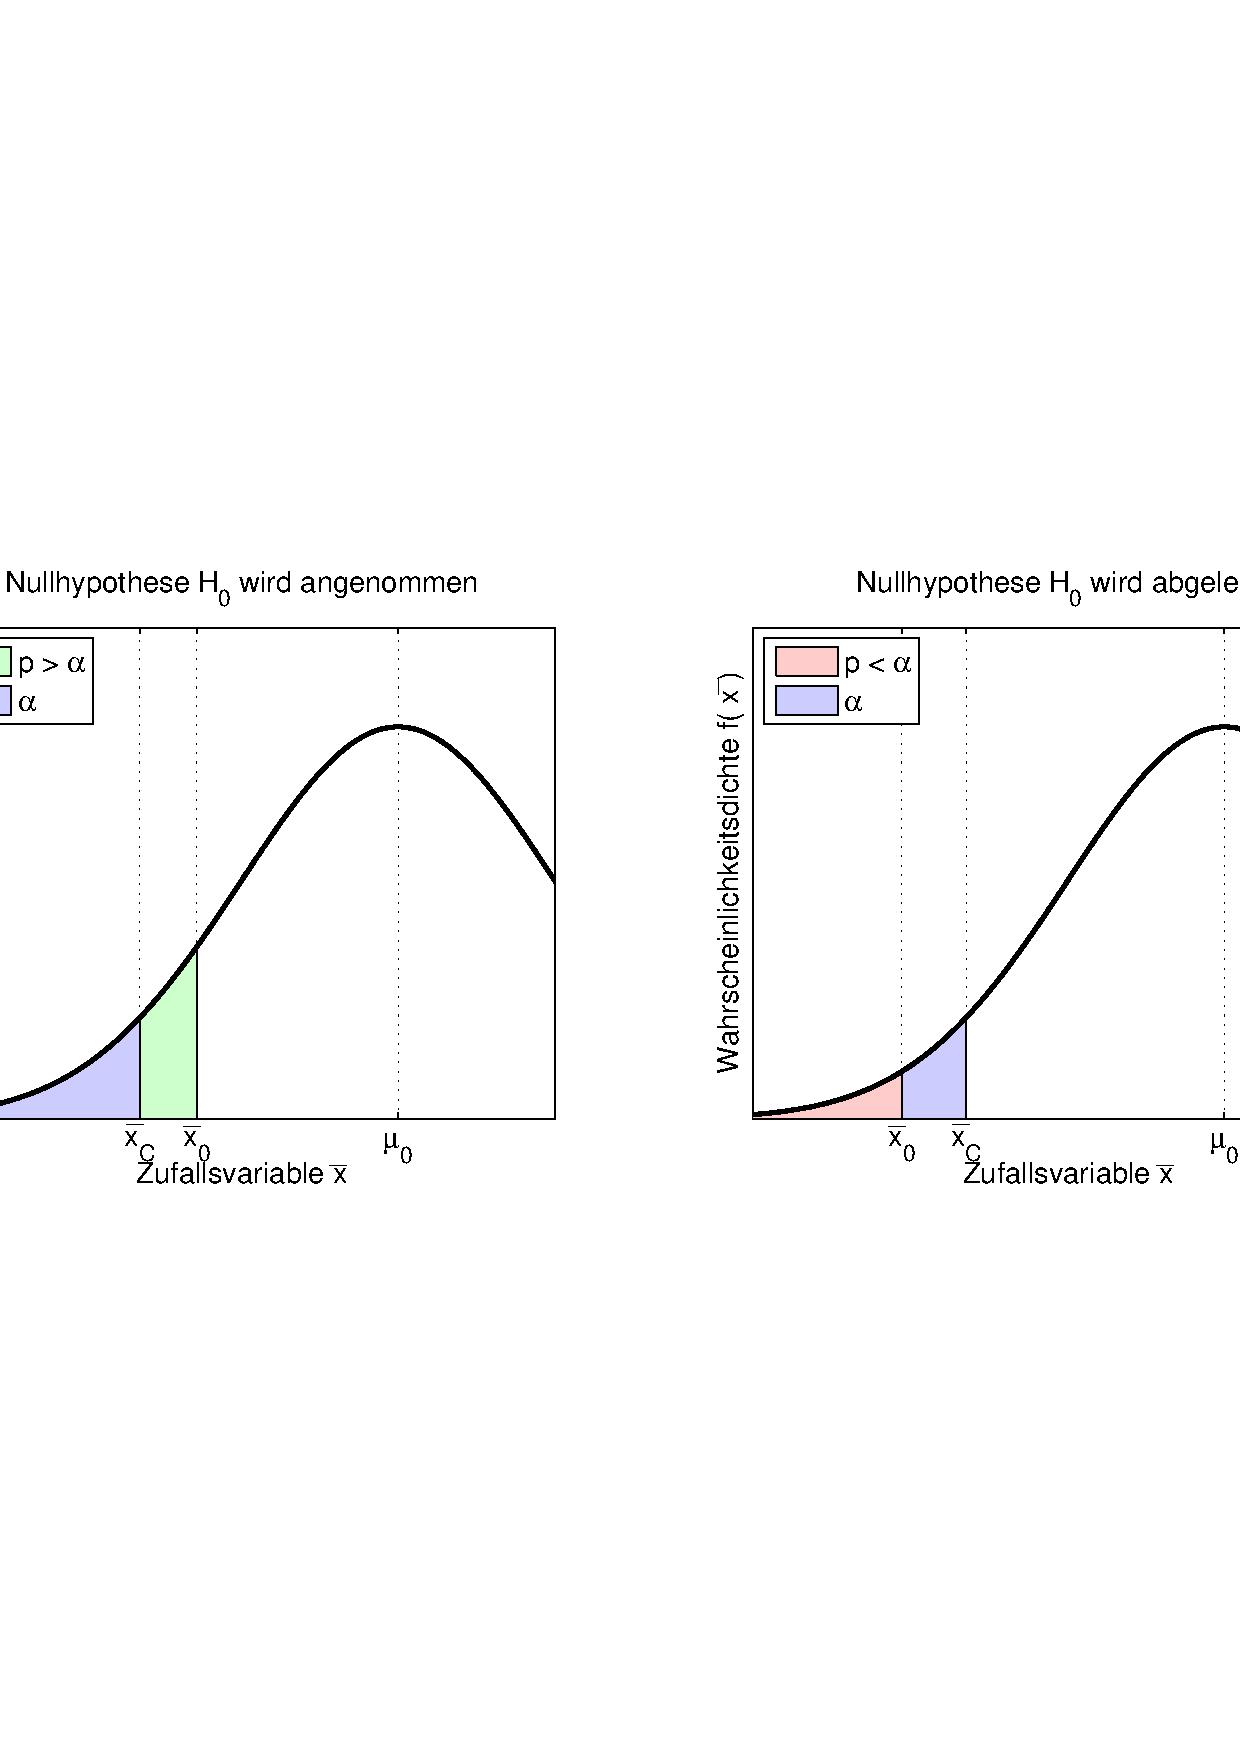
\includegraphics[width=0.3\textwidth]{Kapitel3/Table/image6.png}}}\\ \hline

\parbox[c][1.6in][c]{3.2in}{\centerline{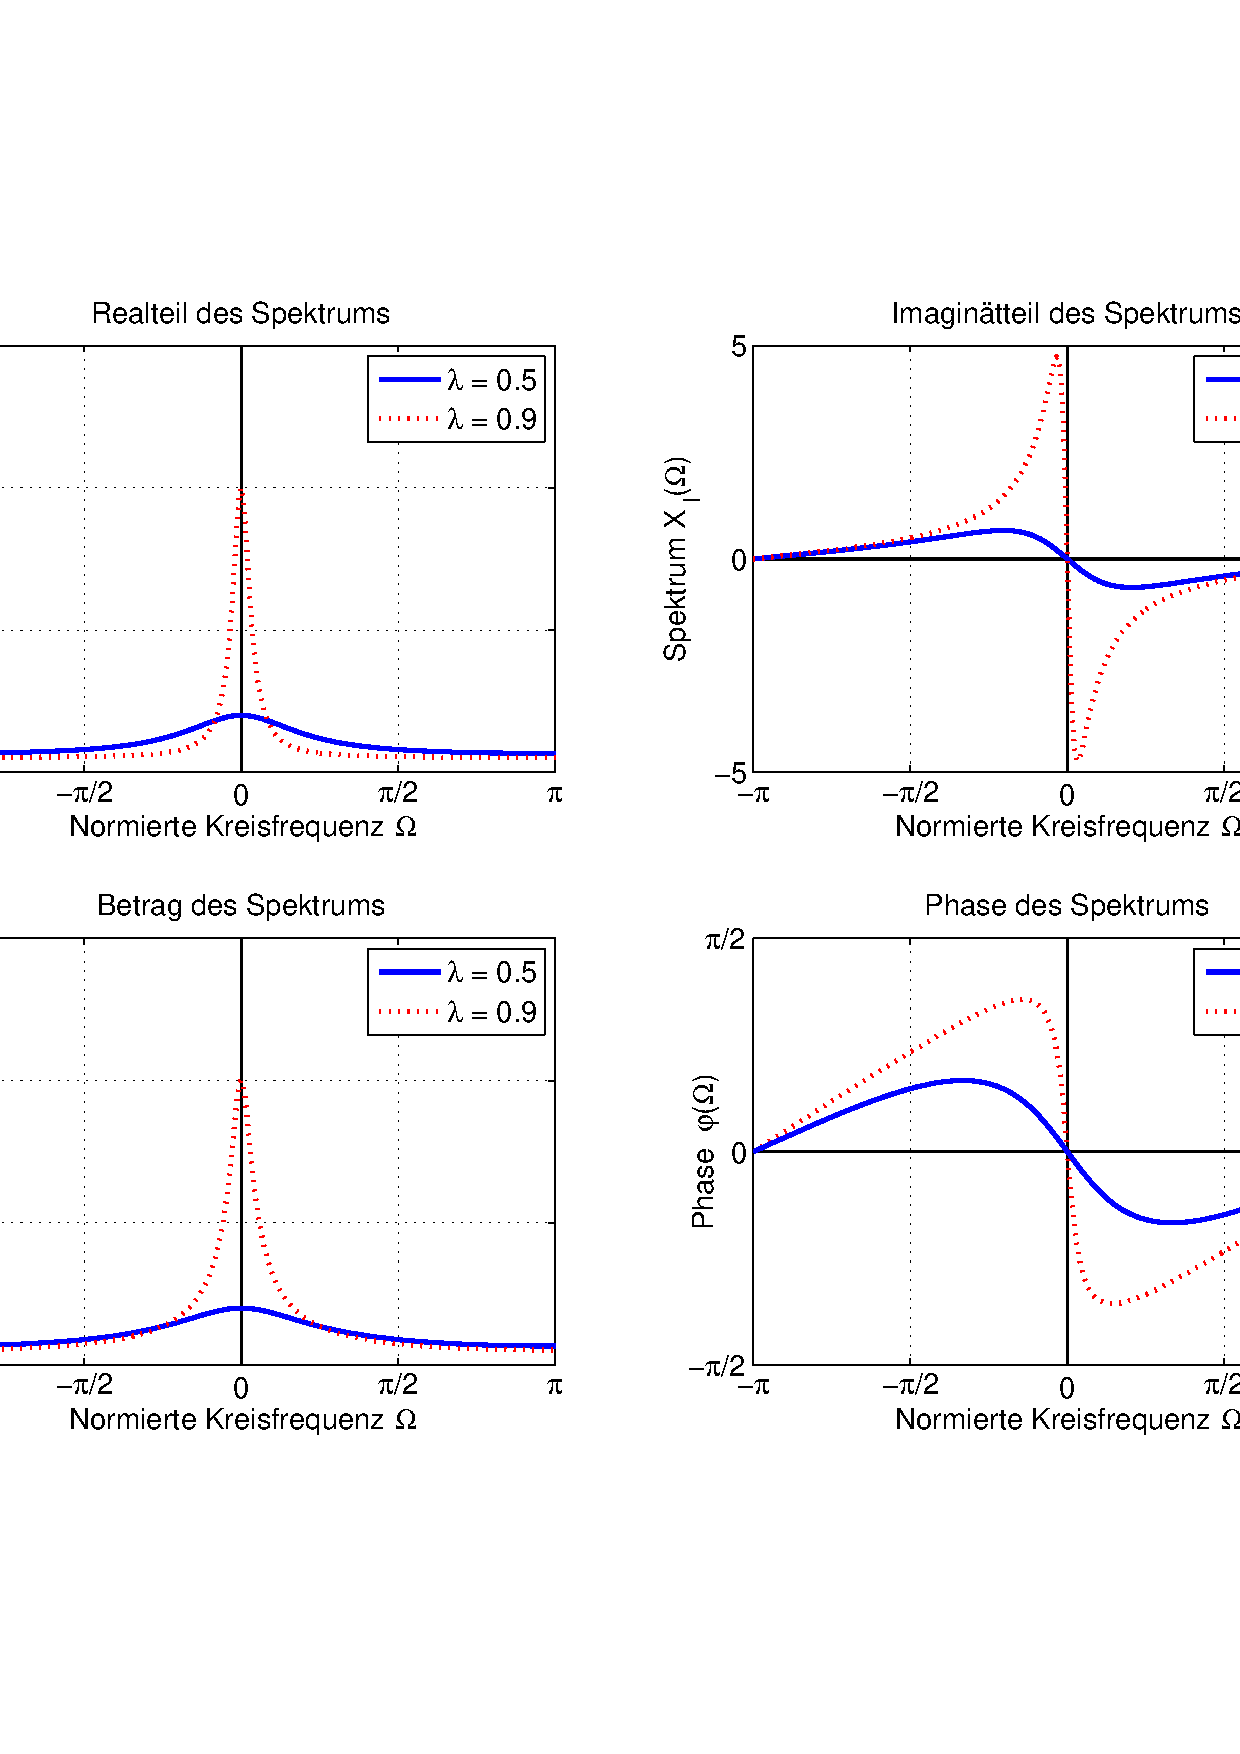
\includegraphics[width=0.3\textwidth]{Kapitel3/Table/image7.png}}} & \parbox[c][1.6in][c]{3.2in}{\centerline{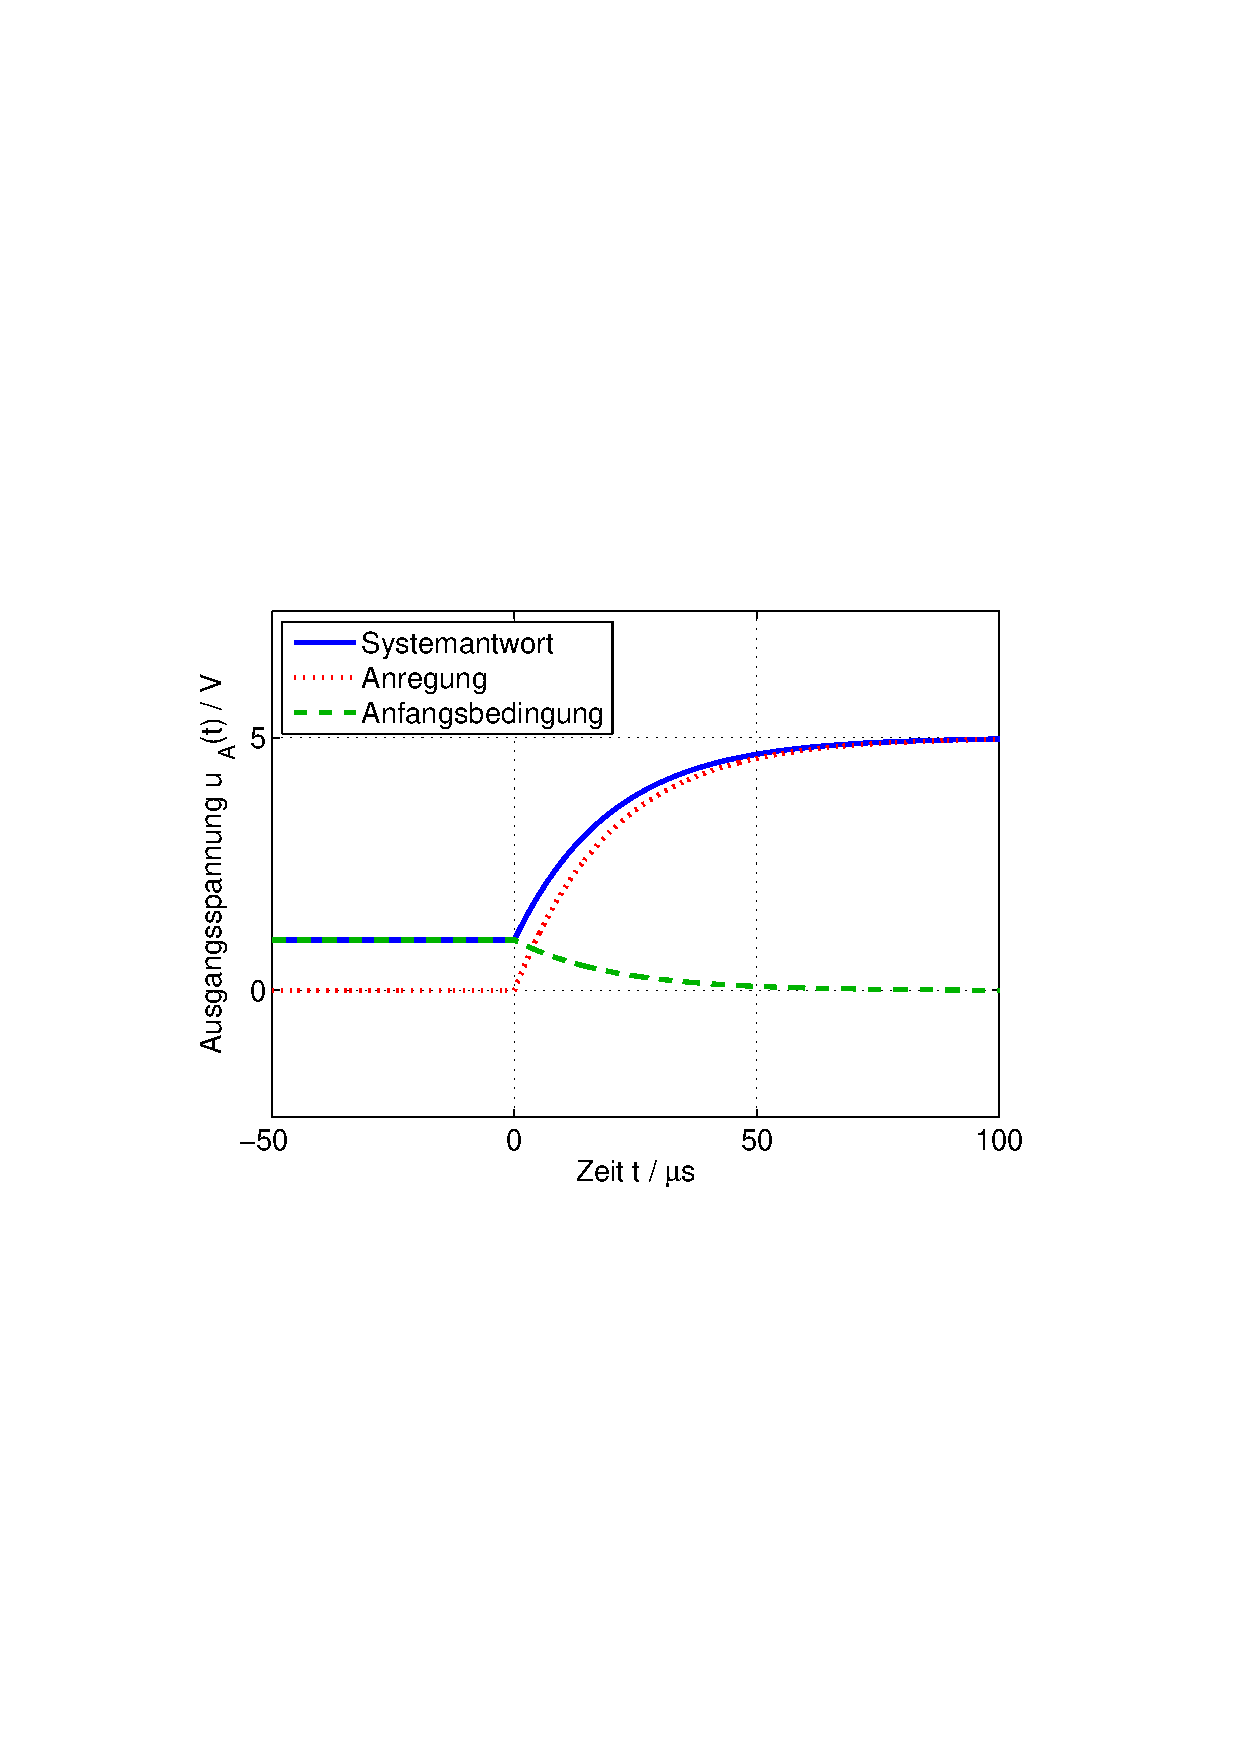
\includegraphics[width=0.3\textwidth]{Kapitel3/Table/image8.png}}}\\ \hline

\parbox[c][1.6in][c]{3.2in}{\centerline{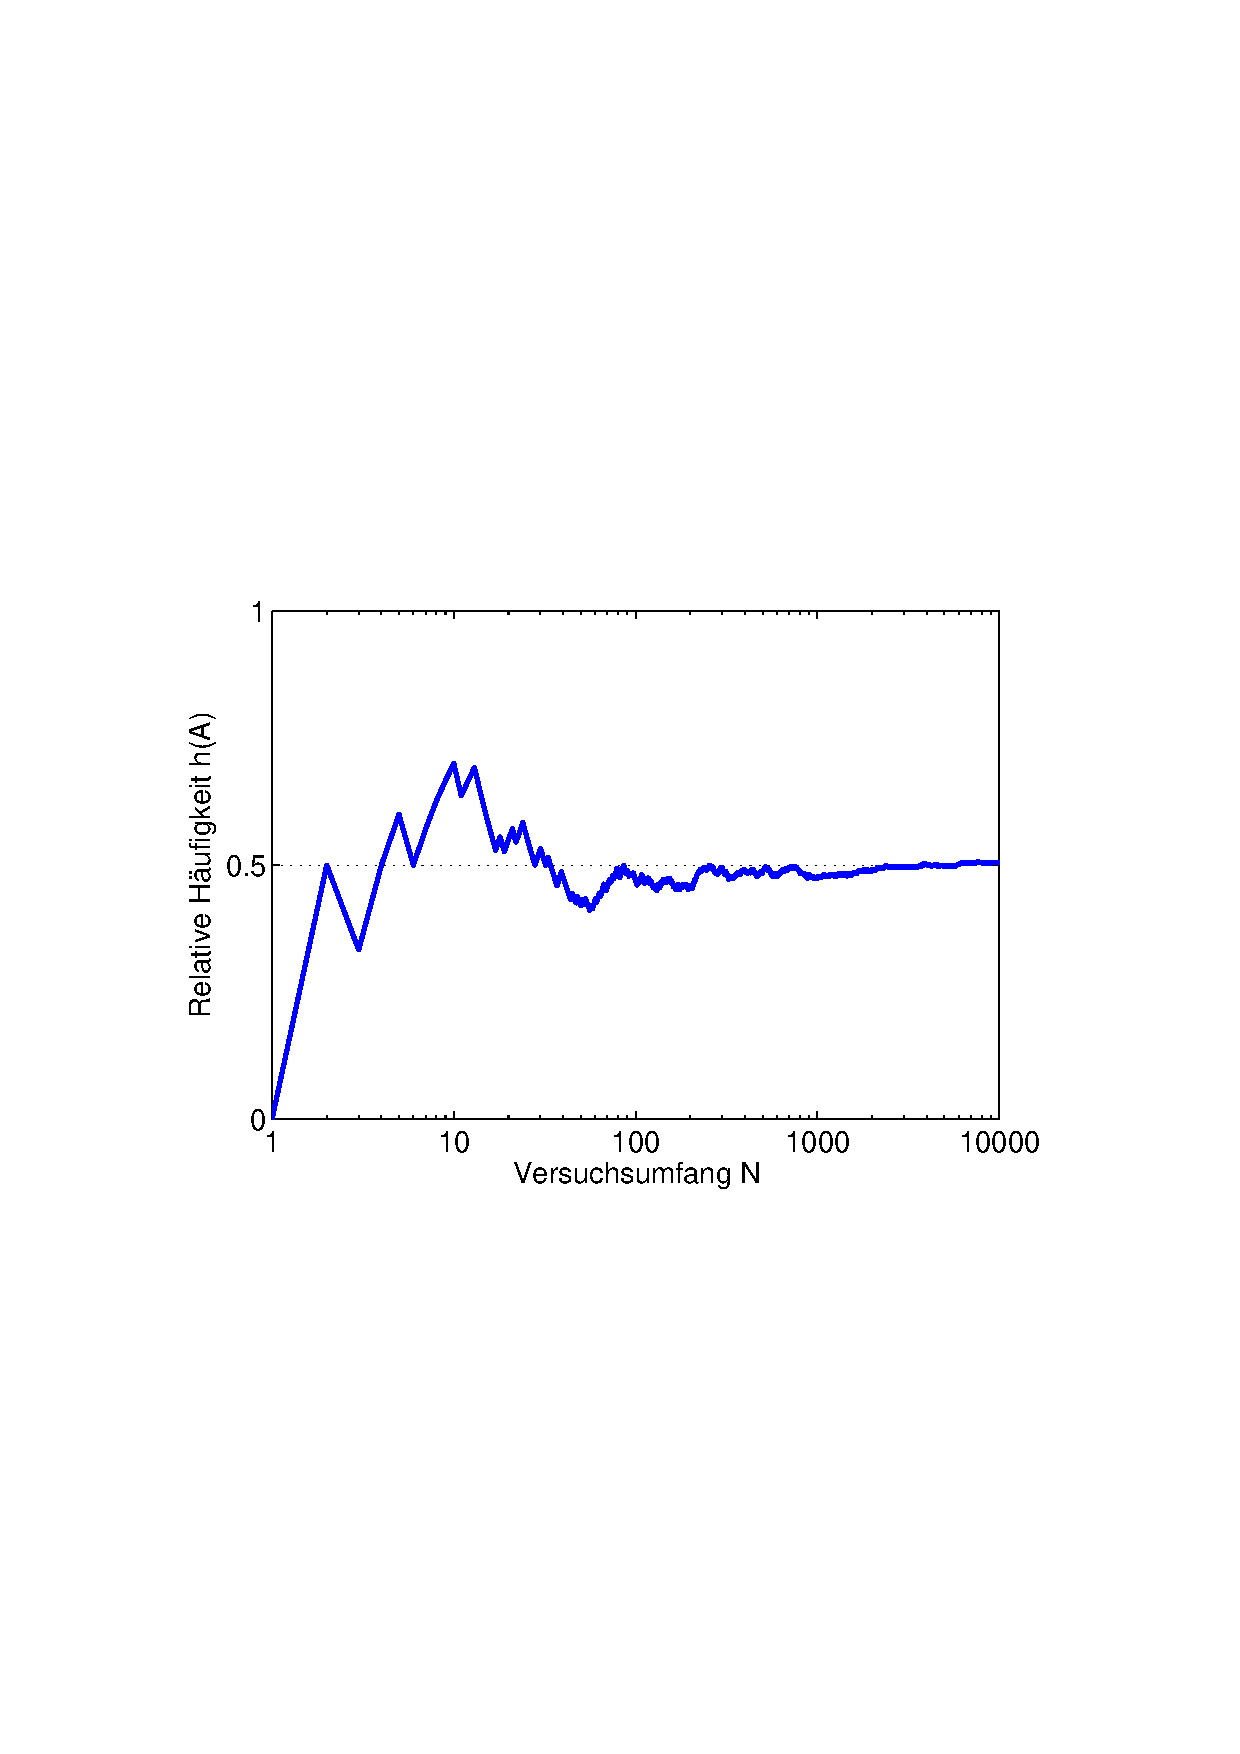
\includegraphics[width=0.3\textwidth]{Kapitel3/Table/image9.png}}} & \parbox[c][1.6in][c]{3.2in}{\centerline{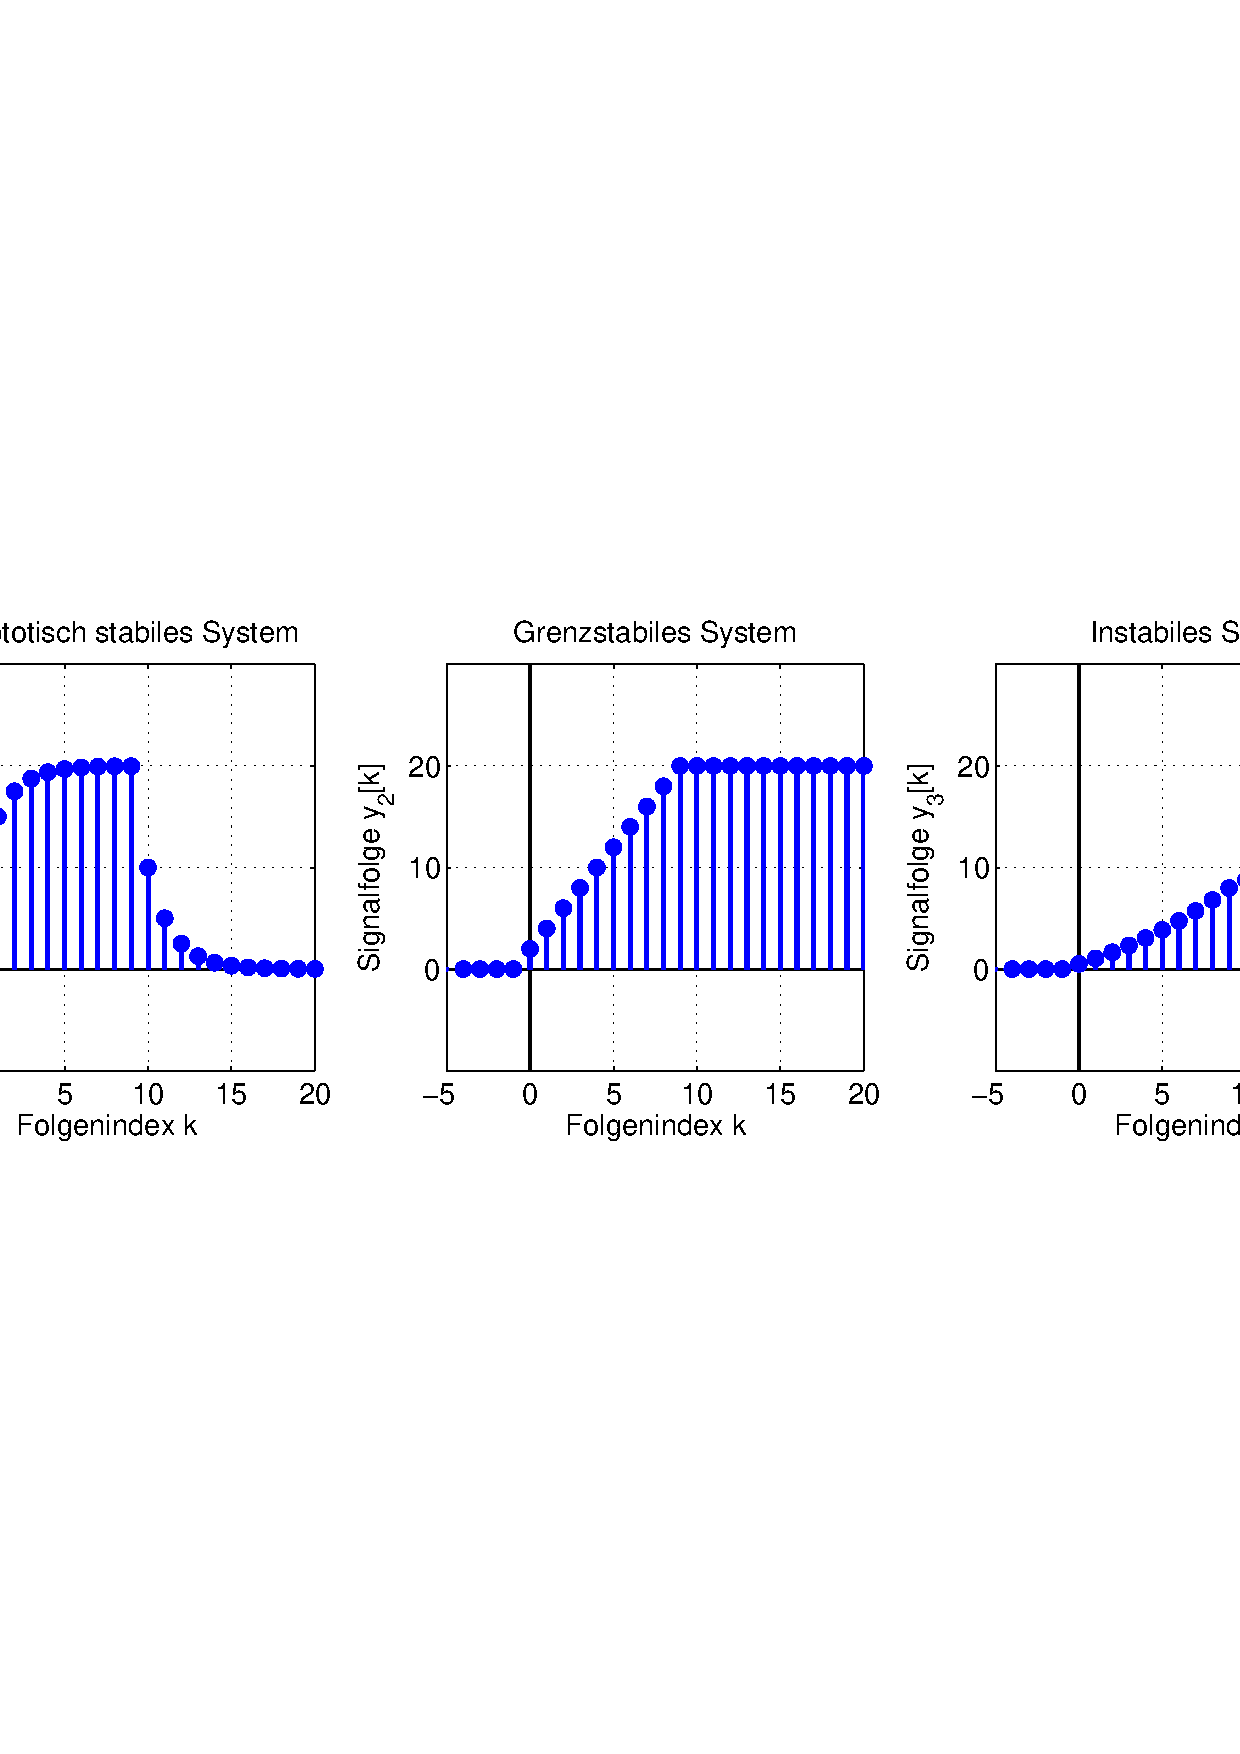
\includegraphics[width=0.3\textwidth]{Kapitel3/Table/image10.png}}}\\ \hline

\parbox[c][1.6in][c]{3.2in}{\centerline{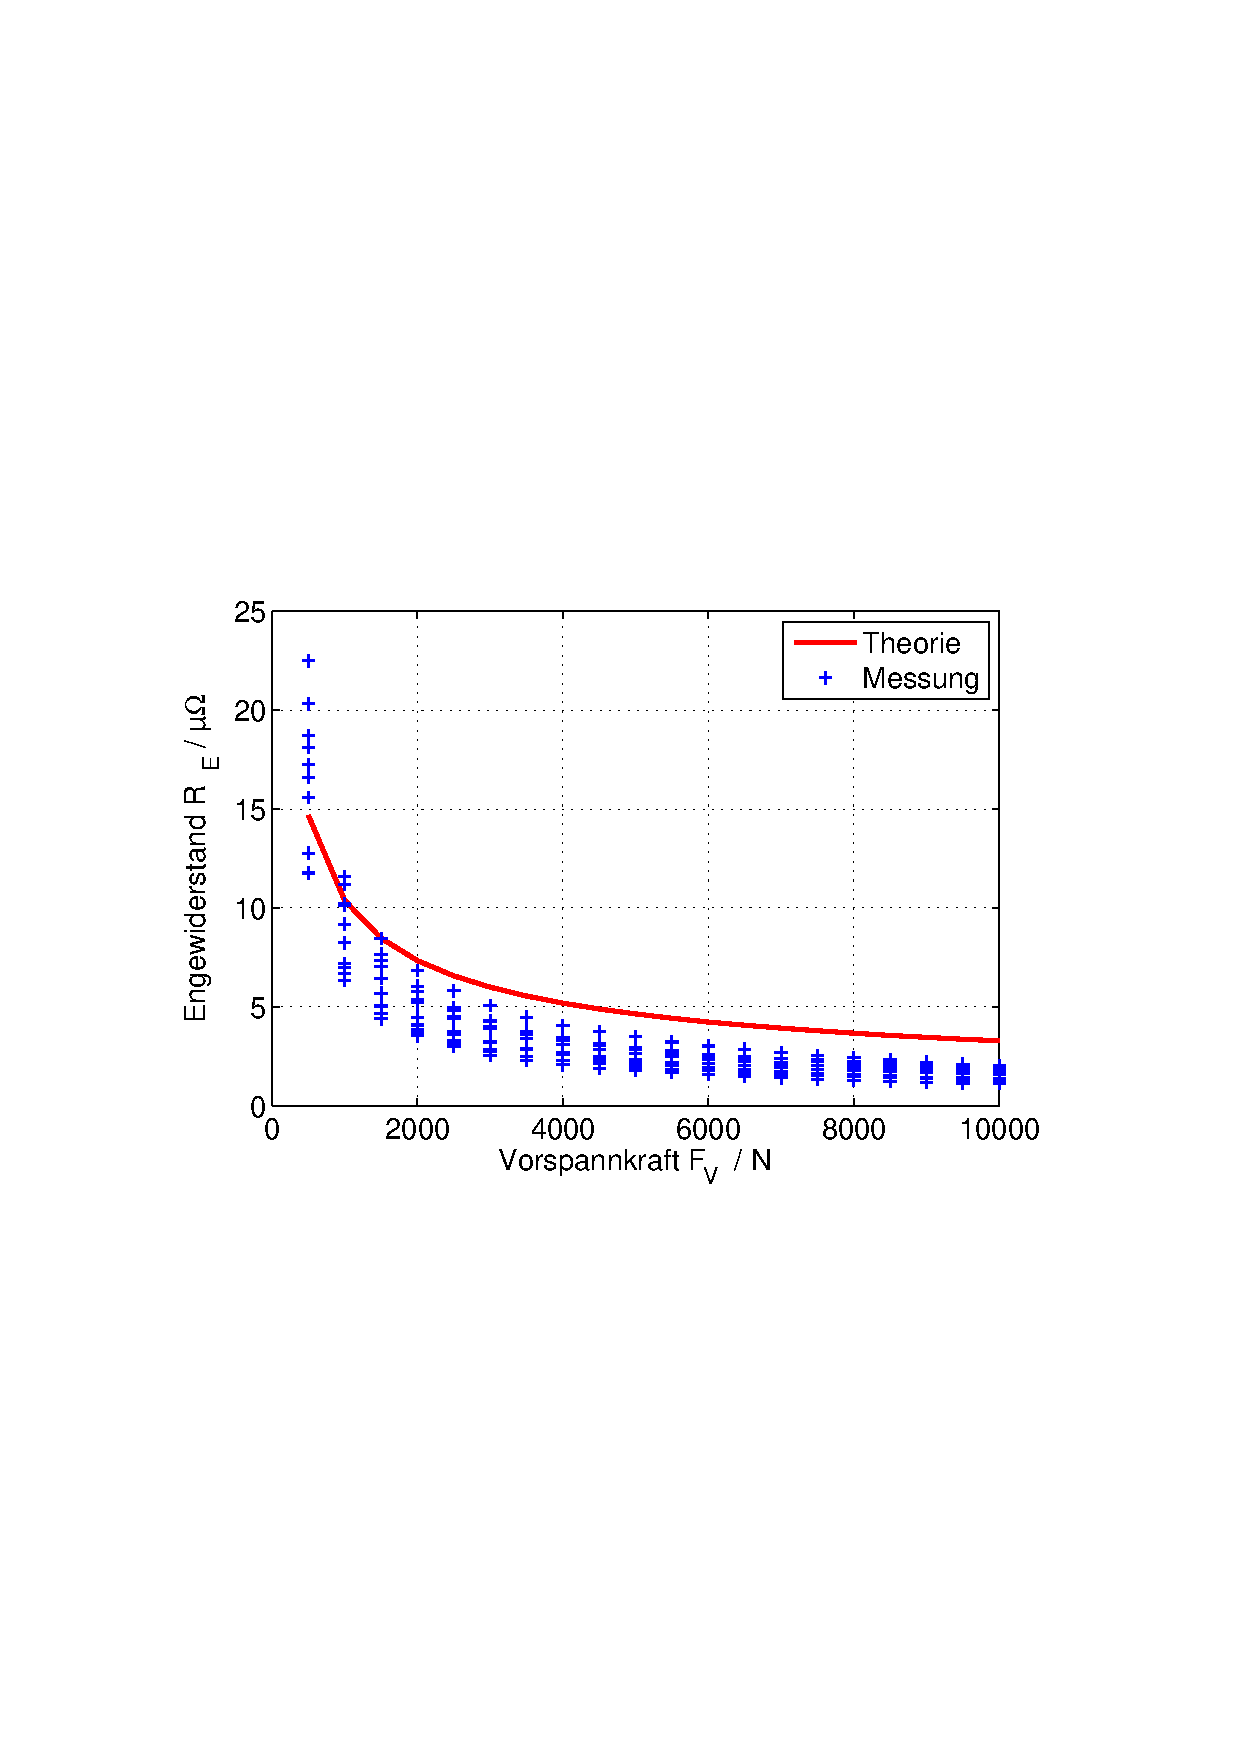
\includegraphics[width=0.3\textwidth]{Kapitel3/Table/image11.png}}} & \parbox[c][1.6in][c]{3.2in}{\centerline{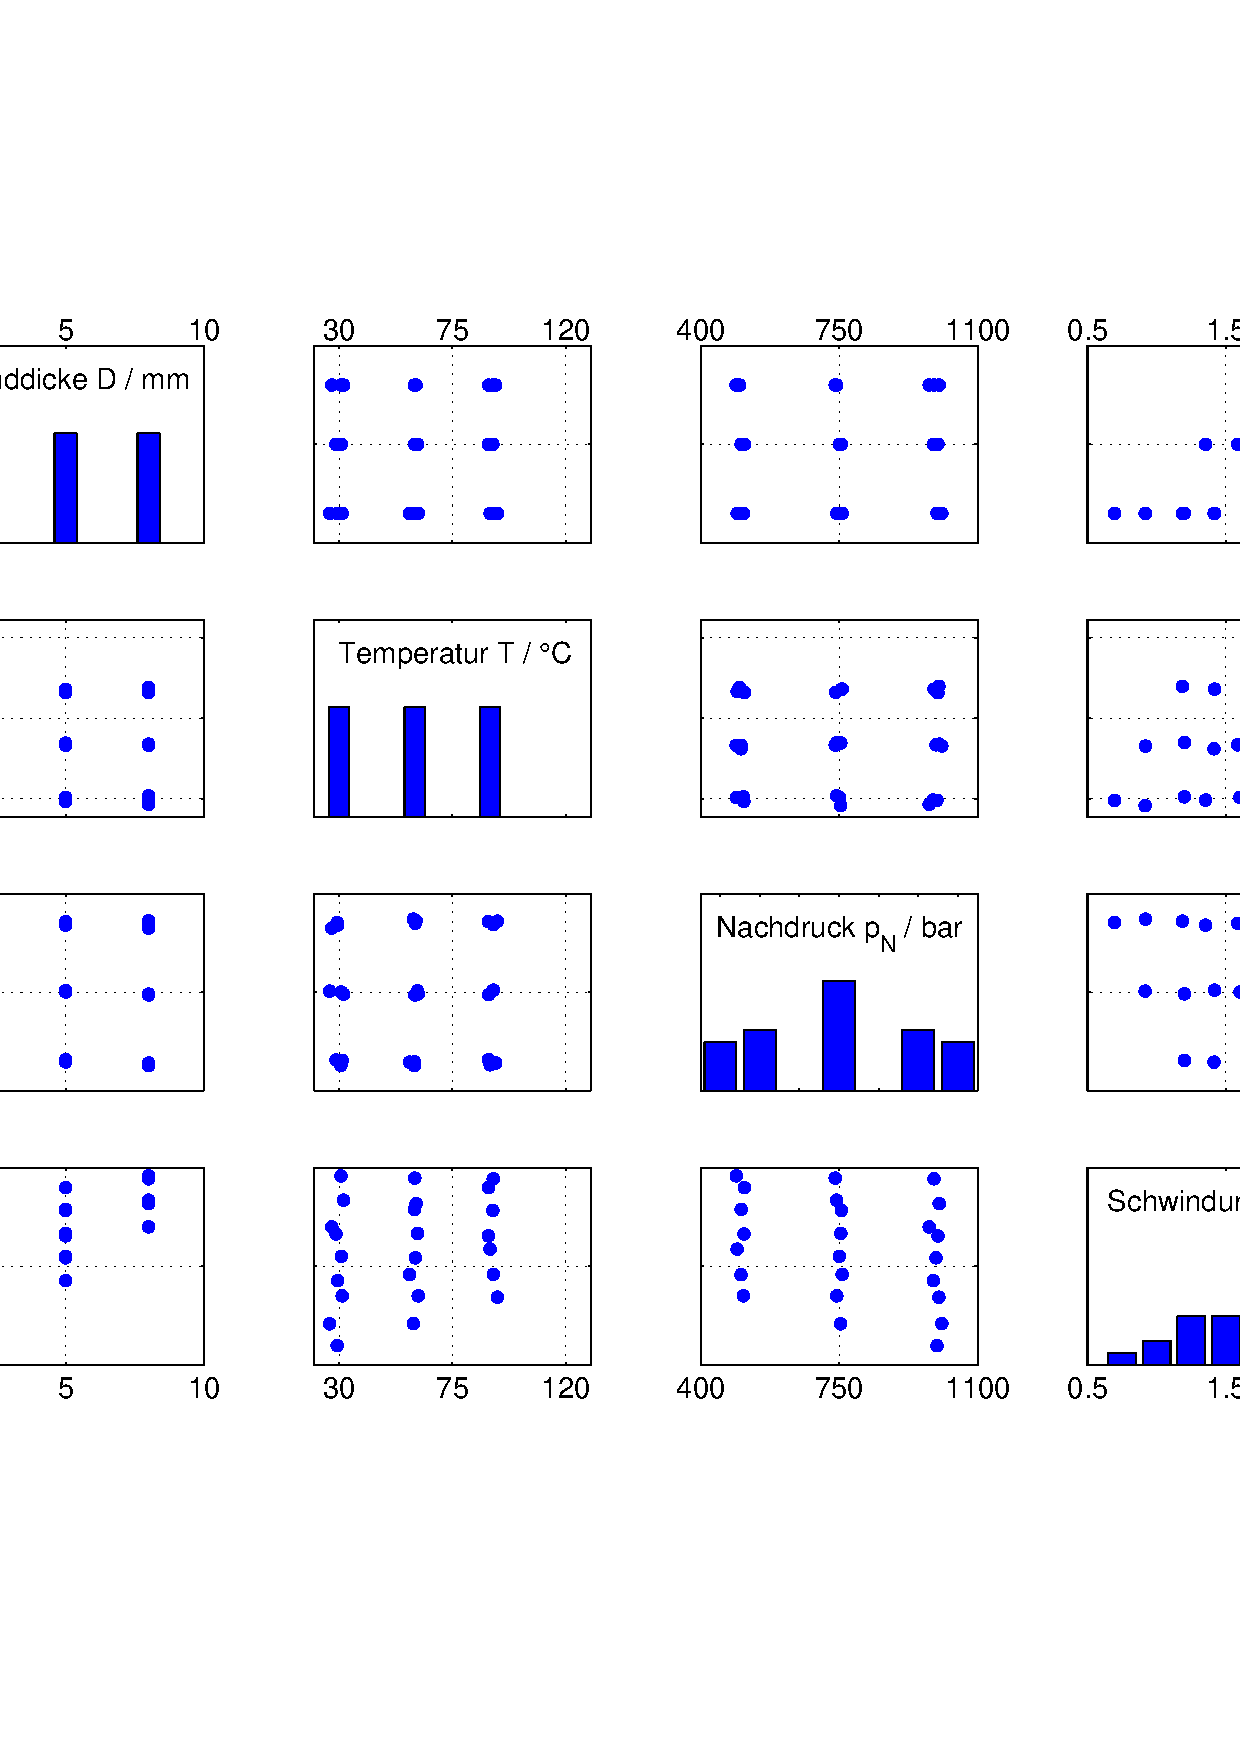
\includegraphics[width=0.3\textwidth]{Kapitel3/Table/image12.png}}}\\ \hline
\end{tabular}%
}
\label{tab:fourone}
\end{table}

\clearpage

\subsection{Rechenregeln der Laplace-Transformation}

\noindent Die Berechnung von Laplace-Transformierten kann über die Auswertung des Laplace-Integrals erfolgen. Dieser Weg ist jedoch oft aufwendig, sodass in der Praxis bereits berechnete Korrespondenzen verwendet werden, um Signale in den Laplace-Bereich zu transformieren. Dazu ist es erforderlich,
Rechenregeln der Laplace-Transformation zu nutzen, um auf standardisierte Ausdrücke zu kommen.
Diese Rechenregeln werden im Folgenden hergeleitet und zusammengefasst. Dabei wird davon ausgegangen, dass die Signale x(t) kausale Signale sind.

\subsubsection{Linearitätsprinzip}

\noindent Die Laplace-Transformation ist eine lineare Transformation. Damit kann eine Linearkombination zweier Funktionen im Laplace-Bereich über dieselbe Linearkombination der jeweiligen Laplace-Transformierten dargestellt werden.

\begin{equation}\label{eq:fourthirty}
L\left\{\nu _{1} \cdot x_{1} \left(t\right)+\nu _{2} \cdot x_{2} \left(t\right)\right\}=\nu _{1} \cdot X_{1} \left(s\right)+\nu _{2} \cdot X_{2} \left(s\right)
\end{equation}

\noindent Der Beweis der Linearität beruht auf der Linearität der Integralrechnung.

\begin{equation}\label{eq:fourthirtyone}
\begin{split}
& L\left\{\nu _{1} \cdot x_{1} \left(t\right)+\nu _{2} \cdot x_{2} \left(t\right)\right\}=\int _{0_{-} }^{\infty }\left(\nu _{1} \cdot x_{1} \left(t\right)+\nu _{2} \cdot x_{2} \left(t\right)\right)\cdot e^{-s\cdot t} {\rm \; } dt \\ 
& =\nu _{1} \cdot \int _{0_{-} }^{\infty }x_{1} \left(t\right)\cdot e^{-s\cdot t} {\rm \; } dt+\nu _{2} \cdot \int _{0_{-} }^{\infty }x_{2} \left(t\right)\cdot e^{-s\cdot t} {\rm \; } dt=\nu _{1} \cdot X_{1} \left(s\right)+\nu _{2} \cdot X_{2} \left(s\right)
\end{split}
\end{equation}\bigskip

\noindent
\colorbox{lightgray}{%
\arrayrulecolor{white}%
\renewcommand\arraystretch{0.6}%
\begin{tabular}{ wl{16.5cm} }
{\fontfamily{phv}\selectfont{Beispiel: Linearität der Laplace-Transformation} }
\end{tabular}%
}\bigskip

\noindent Die Linearitätseigenschaft der Laplace-Transformation kann genutzt werden, um die exponentiell abklingende harmonische Schwingung in den Laplace-Bereich zu transformieren. Sie kann als Summe zweier komplexer Exponentialfunktionen dargestellt werden

\begin{equation}\label{eq:fourthirtytwo}
\begin{split}
x\left(t\right) & = A\cdot e^{\delta \cdot t} \cdot \cos \left(\omega _{0} \cdot t\right)\cdot \sigma \left(t\right)=\frac{1}{2} \cdot A\cdot e^{\delta \cdot t} \cdot \left(e^{j\cdot \omega _{0} \cdot t} +e^{-j\cdot \omega _{0} \cdot t} \right)\cdot \sigma \left(t\right) \\ 
& = {\frac{1}{2} \cdot A\cdot \left(e^{\left(\delta +j\cdot \omega _{0} \right)\cdot t} +e^{\left(\delta -j\cdot \omega _{0} \right)\cdot t} \right)\cdot \sigma \left(t\right)} 
\end{split}
\end{equation}

\noindent Für Exponentialfunktionen ist die Laplace-Transformierte bekannt, sodass die Summe die Laplace-Transformierte

\begin{equation}\label{eq:fourthirtythree}
X\left(s\right)=\frac{1}{2} \cdot A\cdot \left(\frac{1}{s-\left(\delta +j\cdot \omega _{0} \right)} +\frac{1}{s-\left(\delta -j\cdot \omega _{0} \right)} \right)=A\cdot \frac{s-\delta }{\left(s-\delta \right)^{2} +\omega _{0}^{2} } 
\end{equation}

\noindent aufweist. Analog ergibt sich für eine abklingende Sinusfunktion 

\begin{equation}\label{eq:fourthirtyfour}
L\left\{A\cdot e^{\delta \cdot t} \cdot \sin \left(\omega _{0} \cdot t\right)\cdot \sigma \left(t\right)\right\}=A\cdot \frac{\omega _{0} }{\left(s-\delta \right)^{2} +\omega _{0}^{2} }
\end{equation}

\subsubsection{Verschiebungsregel der Zeitfunktion nach rechts, Transport Delay}

\noindent Eine Verschiebung einer Zeitfunktion um t${}_{0}$ nach rechts kann durch x(t - t${}_{0}$) dargestellt werden. Dabei ist t${}_{0}$ eine feste Zahl mit t${}_{0}$ $\mathrm{>}$ 0. F\"{u}r die Funktion im Laplace-Bereich gilt

\begin{equation}\label{eq:fourthirtyfive}
L\left\{x\left(t-t_{0} \right)\right\}=e^{-s\cdot t_{0} } \cdot X\left(s\right)
\end{equation}

\noindent Für den Beweis dieses Verschiebungssatzes wird die Definitionsgleichung der Laplace-Transformation verwendet.

\begin{equation}\label{eq:fourthirtysix}
\begin{split}
L\left\{x\left(t-t_{0} \right)\right\} & = \int\limits _{0_{-} }^{\infty }x\left(t-t_{0} \right)\cdot e^{-s\cdot t}\;dt=\int\limits _{0_{-} }^{\infty }x\left(t-t_{0} \right)\cdot e^{-s\cdot (t-t_{0} )} \cdot e^{-s\cdot t_{0} } \;dt \\ 
& = e^{-s\cdot t_{0} } \cdot \int\limits _{0_{-} }^{\infty }x\left(t-t_{0} \right)\cdot e^{-s\cdot (t-t_{0} )}  \;dt=e^{-s\cdot t_{0} } \cdot \int\limits _{-t_{0} }^{\infty }x\left(t\right)\cdot e^{-s\cdot t}  \;dt \\ 
& = e^{-s\cdot t_{0} } \cdot \int\limits _{-t_{0} }^{0}x\left(t\right)\cdot e^{-s\cdot t} \; dt+e^{-s\cdot t_{0} } \cdot \int\limits _{0_{-} }^{\infty }x\left(t\right)\cdot e^{-s\cdot t}  \;dt
\end{split}
\end{equation}

\noindent Unter der Voraussetzung, dass es sich um ein kausales Signal handelt, ist das erste Integral null, das zweite Integral ist die Laplace-Transformierte X(s) des Zeitsignals x(t). Damit gilt für kausale Signale

\begin{equation}\label{eq:fourthirtyseven}
L\left\{x\left(t-t_{0} \right)\right\}=e^{-s\cdot t_{0} } \cdot X\left(s\right)
\end{equation}

\noindent Der Verschiebung einer kausalen Zeitfunktion um t$_{0}$ nach rechts entspricht eine Multiplikation mit e$^{{\mathrm{-s}\cdot\mathrm{t}}_0}$ im Laplace-Bereich. Eine Verschiebung der Zeitfunktion nach rechts wird bei technischen Anwendungen dazu genutzt, Transportvorg\"{a}nge zu beschreiben. Deshalb hat sich f\"{u}r die Zeitverschiebung der englische Begriff \textit{Transport Delay} durchgesetzt. \bigskip

\noindent
\colorbox{lightgray}{%
\arrayrulecolor{white}%
\renewcommand\arraystretch{0.6}%
\begin{tabular}{ wl{16.5cm} }
{\fontfamily{phv}\selectfont{Beispiel: Verschiebungsregel der Laplace-Transformation}}
\end{tabular}%
}\bigskip

\noindent Die kausale Rechteckfunktion kann durch zwei verschobene Sprungfunktionen dargestellt werden.

\begin{equation}\label{eq:fourthirtyeight}
x\left(t\right)=\sigma \left(t\right)-\sigma \left(t-t_{0} \right)
\end{equation}

\noindent Mit der Verschiebungsregel und der bereits berechneten Korrespondenz der Sprungfunktion

\begin{equation}\label{eq:fourthirtynine}
L\left\{\sigma \left(t\right)\right\}=\frac{1}{s} 
\end{equation}

\noindent ergibt sich die Funktion im Laplace-Bereich

\begin{equation}\label{eq:fourfourty}
X\left(s\right)=\frac{1}{s} -\frac{1}{s} \cdot e^{-s\cdot t_{0} } =\frac{1}{s} \cdot \left(1-e^{-s\cdot t_{0} } \right)
\end{equation}

\noindent Das Ergebnis entspricht dem in Abschnitt 4.1.2 \"{u}ber die Definitionsgleichung der Laplace-Transformation berechneten Ergebnis.

\clearpage

\subsubsection{Modulationsregel}

\noindent Bei der Verschiebungsregel führt eine Verschiebung der Zeitfunktion zu der Multiplikation der Laplace-Transformierten mit einer Exponentialfunktion. Umgekehrt gilt der Zusammenhang

\begin{equation}\label{eq:fourfourtyone}
L\left\{e^{\lambda \cdot t} \cdot x\left(t\right)\right\}=X\left(s-\lambda \right)
\end{equation}

\noindent Dabei ist $\lambda$ eine beliebige komplexe Zahl. Der Beweis beruht wieder auf der Definitionsgleichung des Laplace-Integrals.

\begin{equation}\label{eq:fourfourtytwo}
L\left\{e^{\lambda \cdot t} \cdot x\left(t\right)\right\}=\int\limits _{0_{-} }^{\infty }x\left(t\right)\cdot e^{\lambda \cdot t} \cdot e^{-s\cdot t}\; dt=\int\limits _{0_{-} }^{\infty }x\left(t\right)\cdot e^{-(s-\lambda )\cdot t}\; dt=X\left(s-\lambda \right)
\end{equation}

\noindent Der Multiplikation der Zeitfunktion mit der Exponentialfunktion e$^{\lambda\cdot t}$ entspricht im Laplace-Bereich einer Verschiebung der Funktion um $\lambda$.\bigskip

\noindent
\colorbox{lightgray}{%
\arrayrulecolor{white}%
\renewcommand\arraystretch{0.6}%
\begin{tabular}{ wl{16.5cm} }
{\fontfamily{phv}\selectfont{Beispiel: Modulationsregel der Laplace-Transformation}}
\end{tabular}%
}\bigskip

\noindent Die kausale Sinusfunktion kann mithilfe der Eulerschen Formel dargestellt werden als die Summe von
zwei komplexen Exponentialfunktionen.

\begin{equation}\label{eq:fourfourtythree}
x\left(t\right)=\sin \left(\omega _{0} \cdot t\right)\cdot \sigma \left(t\right)=\frac{1}{2\cdot j} \cdot \left(e^{j\cdot \omega _{0} \cdot t} -e^{-j\cdot \omega _{0} \cdot t} \right)\cdot \sigma \left(t\right)=\frac{1}{2\cdot j} \cdot e^{j\cdot \omega _{0} \cdot t} \cdot \sigma \left(t\right)-\frac{1}{2\cdot j} \cdot e^{-j\cdot \omega _{0} \cdot t} \cdot \sigma \left(t\right)
\end{equation}

\noindent Die Multiplikation der Sprungfunktion mit den Exponentialfunktionen kann als Modulation aufgefasst werden. Mit der Korrespondenz der Sprungfunktion und der Modulationsregel berechnet sich die Korrespondenz der Sinusfunktion zu

\begin{equation}\label{eq:fourfourtyfour}
X\left(s\right)=\frac{1}{2\cdot j} \cdot \frac{1}{s-j\cdot \omega _{0} } -\frac{1}{2\cdot j} \cdot \frac{1}{s+j\cdot \omega _{0} } =\frac{\omega _{0} }{s^{2} +\omega _{0}^{2} }
\end{equation}

\noindent Analog ergibt sich für die Kosinusfunktion

\begin{equation}\label{eq:fourfourtyfive}
L\left\{\cos \left(\omega _{0} \cdot t\right)\cdot \sigma \left(t\right)\right\}=\frac{1}{2} \cdot \frac{1}{s-j\cdot \omega _{0} } +\frac{1}{2} \cdot \frac{1}{s+j\cdot \omega _{0} } =\frac{s}{s^{2} +\omega _{0}^{2} } 
\end{equation}

\subsubsection{Lineare Gewichtung der Zeitfunktion}

\noindent Die Regel zur linearen Gewichtung der Zeitfunktion x(t) ergibt sich durch Ableitung der Laplace-Transformierten X(s) nach der komplexen Variablen s.

\begin{equation}\label{eq:fourfourtysix}
\frac{d}{ds} X\left(s\right)=\frac{d}{ds} \, \, \int\limits _{0_{-} }^{\infty }x\left(t\right)\cdot e^{-s\cdot t} \;dt=\int\limits _{0_{-} }^{\infty }-t\cdot x\left(t\right)\cdot e^{-s\cdot t} \; dt
\end{equation}

\noindent Multiplikation der Gleichung mit - 1 führt zu der Rechenregel der linearen Gewichtung.

\begin{equation}\label{eq:fourfourtyseven}
L\left\{t\cdot x\left(t\right)\right\}=-\frac{dX}{ds} 
\end{equation}\bigskip

\noindent
\colorbox{lightgray}{%
\arrayrulecolor{white}%
\renewcommand\arraystretch{0.6}%
\begin{tabular}{ wl{16.5cm} }
{\fontfamily{phv}\selectfont{Beispiel: Lineare Gewichtung bei der Laplace-Transformation}}
\end{tabular}%
}\bigskip

\noindent Die Laplace-Transformierte der Funktion

\begin{equation}\label{eq:fourfourtyeight}
x\left(t\right)=t\cdot e^{\lambda \cdot t} 
\end{equation}

\noindent kann mit der linearen Gewichtung berechnet werden. Es ergibt sich 

\begin{equation}\label{eq:fourfourtynine}
X\left(s\right)=-\frac{d}{ds} \frac{1}{s-\lambda } =-\frac{d}{ds} \left(s-\lambda \right)^{-1} =\left(s-\lambda \right)^{-2} =\frac{1}{\left(s-\lambda \right)^{2} } 
\end{equation}

\subsubsection{Skalierungsregel}

\noindent Wird die Funktionen x(t) gedehnt oder gestaucht, gilt für die Laplace-Transformierte bei einer reellen Konstante c $\mathrm{>}$ 0

\begin{equation}\label{eq:fourfifty}
L\left\{x\left(c\cdot t\right)\right\}=\frac{1}{c} \cdot X\left(\frac{s}{c} \right)
\end{equation}

\noindent Die Beziehung ergibt sich wieder aus der Integralrechnung.

\begin{equation}\label{eq:fourfiftyone}
L\left\{x\left(c\cdot t\right)\right\}=\int\limits _{0_{-} }^{\infty }x\left(c\cdot t\right)\cdot e^{-s\cdot t} \;  dt=\int\limits _{0_{-} }^{\infty }x\left(c\cdot t\right)\cdot e^{-\frac{s}{c} \cdot c\cdot t} \;  dt
\end{equation}

\noindent Mit der Substitution $\tau$ = c$\cdot$t und d$\tau$/dt = c ergibt die Laplace-Transformierte 

\begin{equation}\label{eq:fourfiftytwo}
L\left\{x\left(c\cdot t\right)\right\}=\int\limits _{0_{-} }^{\infty }x\left(c\cdot t\right)\cdot e^{-\frac{s}{c} \cdot c\cdot t} \; dt=\frac{1}{c} \cdot \int\limits _{0_{-} }^{\infty }x\left(\tau \right)\cdot e^{-\frac{s}{c} \cdot \tau } \; d\tau =\frac{1}{c} \cdot X\left(\frac{s}{c} \right)
\end{equation}

\noindent Analog gilt:

\begin{equation}\label{eq:fourfiftythree}
L\left\{\frac{1}{c} \cdot x\left(\frac{t}{c} \right)\right\}=X\left(c\cdot s\right)
\end{equation}\bigskip

\noindent
\colorbox{lightgray}{%
\arrayrulecolor{white}%
\renewcommand\arraystretch{0.6}%
\begin{tabular}{ wl{16.5cm} }
{\fontfamily{phv}\selectfont{Beispiel: Skalierungsregel der Laplace-Transformation}}
\end{tabular}%
}\bigskip

\noindent Die Rechteckfunktion 

\begin{equation}\label{eq:fourfiftyfour}
x\left(t\right)=\sigma \left(t\right)-\sigma \left(t-t_{0} \right)
\end{equation}

\noindent hat die Laplace-Transformierte 

\begin{equation}\label{eq:fourfiftyfive}
X\left(s\right)=\frac{1}{s} -\frac{1}{s} \cdot e^{-s\cdot t_{0} } =\frac{1}{s} \cdot \left(1-e^{-s\cdot t_{0} } \right)
\end{equation}

\noindent Wird sie um den Faktor 2 gestaucht, 

\begin{equation}\label{eq:fourfiftysix}
y\left(t\right)=x\left(2\cdot t\right)=\sigma \left(2\cdot t\right)-\sigma \left(2\cdot t-t_{0} \right)
\end{equation}

\noindent ergibt sich für die Laplace-Transformierte

\begin{equation}\label{eq:fourfiftyseven}
Y\left(s\right)=\frac{1}{2} \cdot \frac{2}{s} \cdot \left(1-e^{-\frac{s}{2} \cdot t_{0} } \right)=\frac{1}{s} \cdot \left(1-e^{-s\cdot \frac{t_{0} }{2} } \right)
\end{equation}

\noindent Die Gleichung entspricht dem erwarteten Ergebnis, da die Rechteckfunktion bei einer Stauchung um einen Faktor 2 nur noch halb so lang ist, wird die Dauer t$_{0}$ praktisch halbiert.

\subsubsection{Integrationsregel}

\noindent Besitzt die Zeitfunktion x(t) die Laplace-Transformierte X(s), so gilt für ihre Stammfunktion die
Beziehung

\begin{equation}\label{eq:fourfiftyeight}
L\left\{\int\limits _{0_{-} }^{t}x\left(\tau \right)\;d\tau  \right\}=\frac{1}{s} \cdot X\left(s\right)
\end{equation}

\noindent Der Beweis ergibt sich durch Einsetzen des Integralausdrucks in die Definitionsgleichung der Laplace-Transformation

\begin{equation}\label{eq:fourfiftynine}
L\left\{\int\limits _{0_{-} }^{t}x\left(\tau \right)\;d\tau  \right\}=\int\limits _{0_{-} }^{\infty }\int\limits _{0_{-} }^{t}x\left(\tau \right)\;d\tau  \cdot e^{-s\cdot t} \;dt
\end{equation}

\noindent und partielle Integration

\begin{equation}\label{eq:foursixty}
\begin{split}
L\left\{\int\limits _{0_{-} }^{t}x\left(\tau \right)\;d\tau  \right\} & = \int\limits _{0_{-} }^{\infty }\int\limits _{0_{-} }^{t}x\left(\tau \right)\;d\tau  \cdot e^{-s\cdot t} \; dt=\left. \frac{{\rm 1}}{{\rm s}} \cdot e^{-s\cdot t} \cdot \int\limits _{0_{-} }^{t}x\left(\tau \right)\;d\tau  \right|_{0_{-} }^{\infty } -\int\limits _{0_{-} }^{\infty }-\frac{{\rm 1}}{{\rm s}} \cdot x\left(t\right)\cdot e^{-s\cdot t} \; dt \\ 
& = \lim \limits_{t\to \infty } \, \, \frac{{\rm 1}}{{\rm s}} \cdot e^{-s\cdot t} \cdot \int\limits _{0_{-} }^{t}x\left(\tau \right)\;d\tau  -\lim \limits_{t\to 0_{-} } \, \, \frac{{\rm 1}}{{\rm s}} \cdot e^{-s\cdot t} \cdot \int\limits _{0_{-} }^{t}x\left(\tau \right)\;d\tau  +\frac{{\rm 1}}{{\rm s}} \cdot \int\limits _{0_{-} }^{\infty }x\left(t\right)\cdot e^{-s\cdot t}\; dt
\end{split}
\end{equation}

\noindent Für t $\rightarrow$ $\mathrm{\infty}$ wird der erste Summand wegen der Exponentialfunktion zu null, wenn s nur weit genug in der positiven Halbebene liegt und x(t) nicht stärker wächst als eine Exponentialfunktion. Für t = 0$_{-}$ wird der erste Summand zu null, weil die Integrationsgrenzen des Integrals identisch sind. Damit vereinfacht sich der Ausdruck zu

\begin{equation}\label{eq:foursixtyone}
L\left\{\int\limits _{0_{-} }^{t}x\left(\tau \right)\;d\tau  \right\}=\frac{{\rm 1}}{{\rm s}} \cdot \int\limits _{0_{-} }^{\infty }x\left(t\right)\cdot e^{-s\cdot t} \; dt=\frac{{\rm 1}}{{\rm s}} \cdot X\left(s\right)
\end{equation}\bigskip

\noindent
\colorbox{lightgray}{%
\arrayrulecolor{white}%
\renewcommand\arraystretch{0.6}%
\begin{tabular}{ wl{16.5cm} }
{\fontfamily{phv}\selectfont{Beispiel: Integrationsregel der Laplace-Transformation}}
\end{tabular}%
}\bigskip

\noindent Die Rampenfunktion ist die Stammfunktion der Sprungfunktion.

\begin{equation}\label{eq:foursixtytwo}
x\left(t\right)=\int\limits _{0_{-} }^{t}\sigma \left(\tau \right) \; d\tau
\end{equation}

\noindent Mithilfe der Integrationsregel ergibt sich die Laplace-Transformierte der Rampenfunktion zu\bigskip

\begin{equation}\label{eq:foursixtythree}
X\left(s\right)=\frac{1}{s} \cdot \frac{1}{s} =\frac{1}{s^{2} }
\end{equation}

\noindent
\colorbox{lightgray}{%
\arrayrulecolor{white}%
\renewcommand\arraystretch{0.6}%
\begin{tabular}{ wl{16.5cm} }
{\fontfamily{phv}\selectfont{Beispiel: Integrationsregel der Laplace-Transformation}}
\end{tabular}%
}\bigskip

\noindent Die kausale Exponentialfunktion

\begin{equation}\label{eq:foursixtyfour}
x\left(t\right)=e^{\lambda \cdot t} \cdot \sigma \left(t\right)
\end{equation}

\noindent besitzt die Laplace-Transformierte 

\begin{equation}\label{eq:foursixtyfive}
X\left(s\right)=\frac{1}{s-\lambda }
\end{equation}

\noindent Es wird sich zeigen, dass bei der Berechnung von Sprungantworten die Zeitfunktion von Interesse ist, die zu der Laplace-Transformierten

\begin{equation}\label{eq:foursixtysix}
Y\left(s\right)=\frac{1}{s\cdot \left(s-\lambda \right)}
\end{equation}

\noindent gehört. Die zugehörige Zeitfunktion kann mithilfe der Integrationsregel bestimmt werden zu

\begin{equation}\label{eq:foursixtyseven}
y\left(t\right)=\int\limits _{0_{-} }^{t}e^{\lambda \cdot \tau } \cdot \sigma \left(\tau \right) \; d\tau =\int _{0_{-} }^{t}e^{\lambda \cdot \tau }  \; d\tau =\left. \frac{1}{\lambda } \cdot e^{\lambda \cdot \tau } \right|_{0_{-} }^{t} =\frac{1}{\lambda } \cdot \left(e^{\lambda \cdot t} -1\right)
\end{equation}

\subsubsection{Differentiationsregel}\label{fourtwoseven}

\noindent Besitzt die Zeitfunktion x(t) die Laplace-Transformierte X(s), so gilt für ihre verallgemeinerte Ableitung die Beziehung

\begin{equation}\label{eq:foursixtyeight}
L\left\{\frac{dx}{dt} \right\}=s\cdot X\left(s\right)-x\left(0_{-} \right)
\end{equation}

\noindent Zur Herleitung der Differentiationsregel für die verallgemeinerte Differentiation wird daran erinnert, dass die Funktion x(t) einen stetigen Anteil x$_{S}$(t) und einen Sprung $\Delta$x an der Stelle t = 0 haben kann. Zun\"{a}chst wird die Differentiationsregel für stetige Funktionen hergeleitet. Durch Einsetzen in die Definitionsgleichung der Laplace-Transformation ergibt sich

\begin{equation}\label{eq:foursixtynine}
L\left\{\frac{dx}{dt} \right\}=\int\limits _{0_{-} }^{\infty }\frac{dx}{dt}  \cdot e^{-s\cdot t} \;dt
\end{equation}

\noindent Mit partieller Integration ergibt sich 

\begin{equation}\label{eq:fourseventy}
L\left\{\frac{dx}{dt} \right\}=\int\limits _{0_{-} }^{\infty }\frac{dx}{dt}  \cdot e^{-s\cdot t} \;dt=\left. x\left(t\right)\cdot e^{-s\cdot t} \right|_{0_{-} }^{\infty } +s\cdot \int\limits _{0_{-} }^{\infty }x\left(t\right)\cdot e^{-s\cdot t} \;dt
\end{equation}

\noindent Der erste Summand geht für t $\rightarrow$ $\mathrm{\infty}$ gegen null, wenn s nur weit genug in der positiven Halbebene liegt und x(t) nicht stärker wächst als eine Exponentialfunktion. Damit vereinfacht sich der Ausdruck zu

\begin{equation}\label{eq:fourseventyone}
L\left\{\frac{dx}{dt} \right\}=-x\left(0_{-} \right)+s\cdot X\left(s\right)=s\cdot X\left(s\right)-x\left(0_{-} \right)
\end{equation}

\noindent Dabei kennzeichnet der Ausdruck x(0$_{-}$) den linksseitigen Grenzwert von x(t) an der Stelle t = 0. Entsprechend ergibt sich für höhere Ableitungen in t die Laplace-Transformierte

\begin{equation}\label{eq:fourseventytwo}
L\left\{\frac{d^{n} x}{dt^{n} } \right\}=s^{n} \cdot X\left(s\right)-s^{n-1} \cdot x\left(0_{-} \right)-...-\left. \frac{d^{n-1} x}{dt^{n-1} } \right|_{t=0_{-} }
\end{equation}

\noindent F\"{u}r die zweite und dritte Ableitung ergibt sich

\begin{equation}\label{eq:fourseventythree}
L\left\{\frac{d^{2} x}{dt^{2} } \right\}=s^{2} \cdot X\left(s\right)-s\cdot x\left(0_{-} \right)-\left. \frac{dx}{dt} \right|_{t=0_{-} }
\end{equation}

\noindent und

\begin{equation}\label{eq:fourseventyfour}
L\left\{\frac{d^{3} x}{dt^{3} } \right\}=s^{3} \cdot X\left(s\right)-s^{2} \cdot x\left(0_{-} \right)-s\cdot \left. \frac{dx}{dt} \right|_{t=0_{-} } -\left. \frac{d^{2} x}{dt^{2} } \right|_{t=0_{-} } 
\end{equation}

\noindent Die Ableitungsregel ist für praktische Anwendungen der Laplace-Transformation die wichtigste. Sie drückt aus, dass die Differentiation im Zeitbereich in eine Multiplikation im Laplace-Bereich übergeht. Sie ist damit Voraussetzung für die vergleichsweise einfache Lösung von linearen Differentialgleichungen mit Anfangsbedingungen.\bigskip

\noindent
\colorbox{lightgray}{%
\arrayrulecolor{white}%
\renewcommand\arraystretch{0.6}%
\begin{tabular}{ wl{16.5cm} }
{\fontfamily{phv}\selectfont{Beispiel: Ableitungsregel der Laplace-Transformation}}
\end{tabular}%
}\bigskip

\noindent In Abschnitt \ref{threeoneone} wird die Ausgangsspannung eines RC-Netzwerks berechnet, das mit einem Spannungssprung angeregt wird. Dieses Beispiel wird hier erneut aufgegriffen.

\begin{figure}[H]
  \centerline{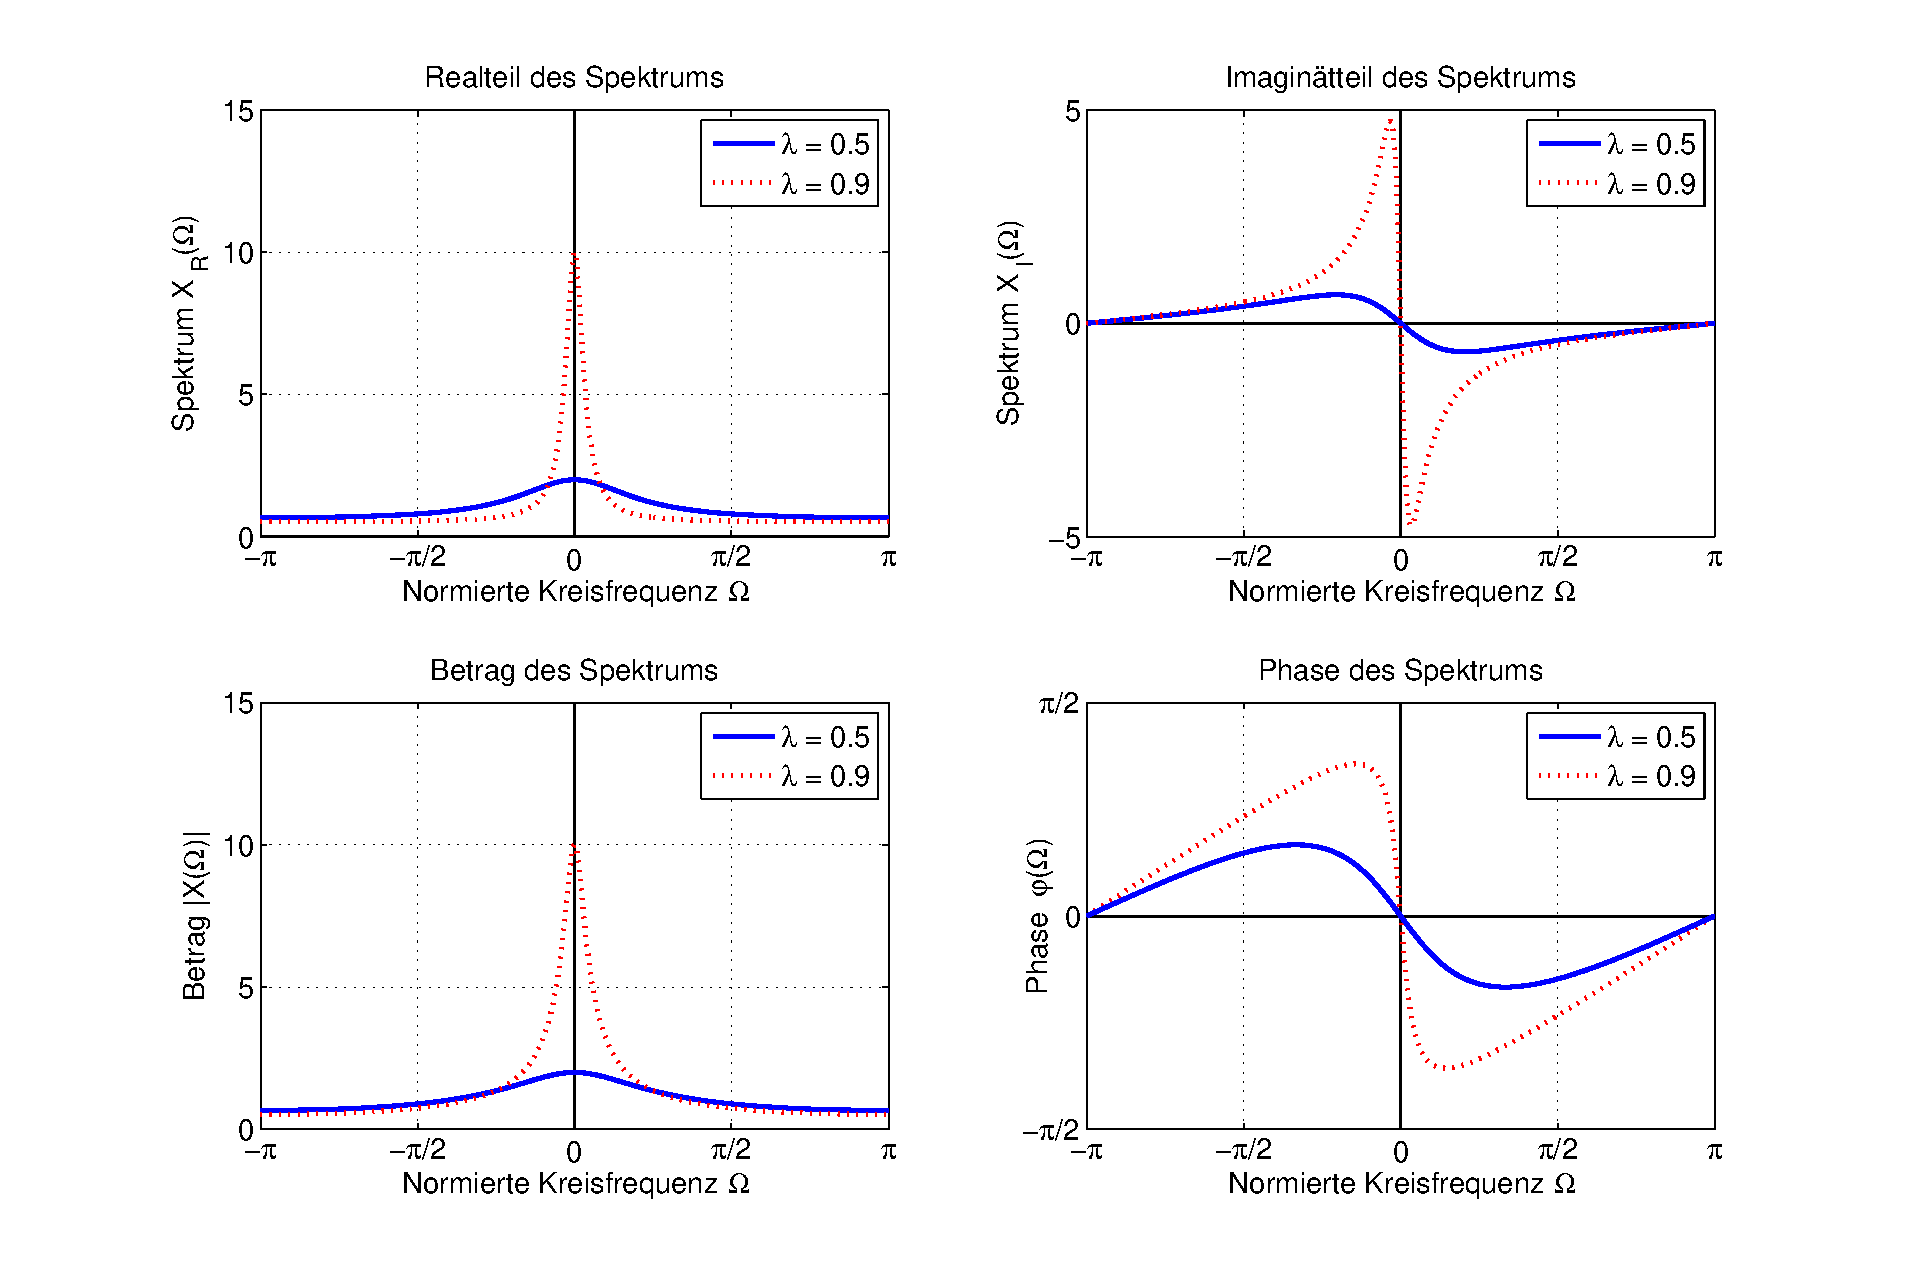
\includegraphics[width=0.4\textwidth]{Kapitel3/Bilder/image7}}
  \caption{Schaltbild für das Beispiel RC-Netzwerk}
  \label{fig:fourRCSchaltbild}
\end{figure}

\noindent Die Ausgangsspannung ergibt sich aus der Differentialgleichung:

\begin{equation}\label{eq:fourseventyfive}
R\cdot C\cdot \frac{du_{A} }{dt} +u_{A} \left(t\right)=u_{E} \left(t\right)
\end{equation}

\noindent Mit der Laplace-Transformation ergibt sich unter Anwendung der Linearitäts- und der Ableitungsregel 

\begin{equation}\label{eq:fourseventysix}
R\cdot C\cdot \left(s\cdot U_{A} \left(s\right)-u_{A} \left(0_{-} \right)\right)+U_{A} \left(s\right)=U_{A} \left(s\right)
\end{equation}

\noindent Wie in Abschnitt \ref{threeoneone} wird die Ausgangsspannung für einen Spannungssprung zum Zeitpunkt t = 0 von 5 V berechnet und eine Spannung am Kondensator von u${}_{A}$(0${}_{-}$) = U${}_{A0}$ angenommen. Damit ergibt sich für das Eingangssignal U${}_{E}$(s) im Laplace-Bereich

\begin{equation}\label{eq:fourseventyseven}
U_{E} \left(s\right)=\frac{5\;V}{s}
\end{equation}

\noindent Einsetzen in Gleichung (\eqref{eq:fourseventysix}) f\"{u}hrt zu der Gleichung

\begin{equation}\label{eq:fourseventyeight}
R\cdot C\cdot \left(s\cdot U_{A} \left(s\right)-U_{A0} \right)+U_{A} \left(s\right)=\frac{5\;V}{s}
\end{equation}

\noindent Ausmultiplizieren und Auflösen nach U$_{A}$(s) ergibt

\begin{equation}\label{eq:fourseventynine}
R\cdot C\cdot s\cdot U_{A} \left(s\right)+U_{A} \left(s\right)=\frac{5\;V}{s} +R\cdot C\cdot U_{A0} 
\end{equation}

\noindent beziehungsweise

\begin{equation}\label{eq:foureighty}
U_{A} \left(s\right)=\frac{5\;V}{s\cdot \left(1+R\cdot C\cdot s\right)} +\frac{R\cdot C}{1+R\cdot C\cdot s} \cdot U_{A0} 
\end{equation}

\noindent Bei der Rücktransformation müssen zwei Summanden berücksichtigt werden. Die Ausgangsspannung u$_{A}$(t) ergibt sich mit den bereits berechneten Korrespondenzen zu

\begin{equation}\label{eq:foureightyone}
u_{A} \left(t\right)=5\;V\cdot \left(1-e^{-\frac{t}{R\cdot C} } \right)\cdot \sigma \left(t\right)+U_{A0} \cdot e^{-\frac{t}{R\cdot C} } \cdot \sigma \left(t\right) 
\end{equation}

\noindent Damit ist das Ergebnis in Gleichung \eqref{eq:fourseven} bestätigt. Bild \ref{fig:LaplaceSignaleRCEinschwingen} stellt das Einschwingverhalten der Kondensatorspannung u$_{A}$(t) für eine Spannung U$_{E}$= 5 V, eine Spannung U${}_{A0}$ = 1 V, einen Widerstand R = 5 k$\Omega$ und eine Kapazität C = 4 nF dar.

\begin{figure}[H]
  \centerline{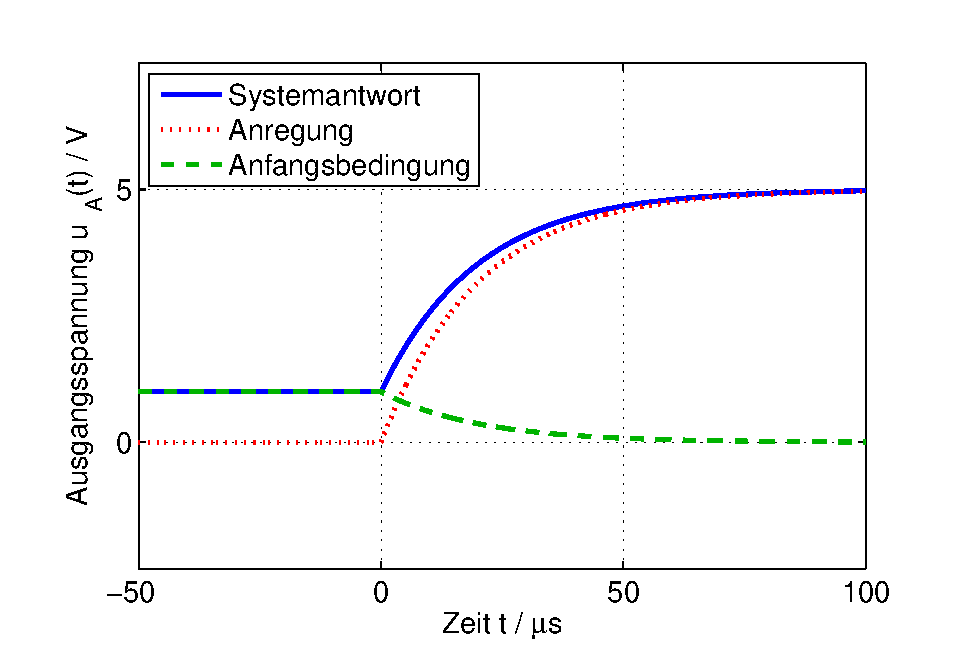
\includegraphics[width=0.5\textwidth]{Kapitel3/Bilder/image8}}
  \caption{Einschwingverhalten der Kondensatorspannung u$_{A}$  bei Anregung 
mit einem Spannungssprung \newline von U$_{E}$ = 5 V und einer Anfangsbedingung von U$_{A0}$ = 1 V
}
  \label{fig:LaplaceSignaleRCEinschwingen}
\end{figure}

\noindent Bereits an diesem einfachen Beispiel zeigt sich der Vorteil der Laplace-Transformation. Sie ermöglicht eine schnelle Berechnung von Systemantworten linearer, zeitinvarianter Systeme unter Berücksichtigung von Anfangsbedingungen.

\subsubsection{Multiplikation zweier Zeitfunktionen}

\noindent Die Rechenregel zur Multiplikation zweier Zeitfunktionen wird in Abschnitt \ref{fourthreeone} über das Umkehrintegral der Laplace-Transformation hergeleitet. Sie wird hier der Vollständigkeit halber aufgeführt.

\begin{equation}\label{eq:foureightytwo}
L\left\{x\left(t\right)\cdot w\left(t\right)\right\}=\frac{1}{2\cdot \pi \cdot j} \int\limits _{c-j\cdot \infty }^{c+j\cdot \infty }X\left(\upsilon \right)\cdot W\left(s-\upsilon \right)\;d\upsilon  =X\left(s\right)*W\left(s\right)
\end{equation}

\noindent Die Multiplikation im Zeitbereich führt zu der Faltung der entsprechenden Laplace-Transformierten im Laplace-Bereich. Diese Rechenregel ist zum Beispiel bei Modulationsverfahren und bei der Fensterung von Signalen von Bedeutung.

\subsubsection{Faltung zweier Zeitfunktionen}

\noindent Bei der Berechnung der Systemantwort y(t) im Zeitbereich wird die Faltungsoperation verwendet. Im Laplace-Bereich berechnet sich die Systemantwort Y(s) aus dem Produkt der einzelnen Laplace-
Transformierten G(s) und U(s).

\begin{equation}\label{eq:foureightythree}
L\left\{g\left(t\right)*u\left(t\right)\right\}=G\left(s\right)\cdot U\left(s\right)
\end{equation}

\noindent Für den Beweis dieser Rechenregel wird von dem Produkt der beiden Laplace-Transformierten ausgegangen.

\begin{equation}\label{eq:foureightyfour}
\begin{split}
G\left(s\right)\cdot U\left(s\right) & = \int\limits _{0_{-} }^{\infty }u\left(\upsilon \right)\cdot e^{-s\cdot \upsilon } \; d\upsilon  \cdot \int\limits _{0_{-} }^{\infty }g\left(\tau \right)\cdot e^{-s\cdot \tau } \;d\tau  =\int\limits _{0_{-} }^{\infty }\int\limits _{0_{-} }^{\infty }u\left(\upsilon \right)\cdot e^{-s\cdot \upsilon } \cdot g\left(\tau \right)\cdot e^{-s\tau } \; d\tau\;\upsilon \\
& = \int\limits _{0_{-} }^{\infty }g\left(\tau \right)\cdot  \int\limits _{0_{-} }^{\infty } u(\upsilon)\cdot e^{-s\cdot( \upsilon + \tau) } d\upsilon d\tau 
\end{split}
\end{equation}

\noindent Mit der Substitution

\begin{equation}\label{eq:foureightyfive}
\upsilon + \tau = t
\end{equation}

\noindent und der Ableitung

\begin{equation}\label{eq:foureightysix}
\frac{d\upsilon }{dt} =1
\end{equation}

\noindent ergibt sich

\begin{equation}\label{eq:foureightyseven}
G\left(s\right)\cdot U\left(s\right)=\int\limits _{0_{-} }^{\infty }g\left(\tau \right)\cdot \int\limits _{0_{-} }^{\infty }u\left(\upsilon \right)\cdot e^{-s\cdot (\upsilon +\tau )} \;d\upsilon \;d\tau   =\int\limits _{0_{-} }^{\infty }g\left(\tau \right)\cdot \int\limits _{\tau _{-} }^{\infty }u\left(t-\tau \right)\cdot e^{-s\cdot t} \;dt\;d\tau  
\end{equation}

\noindent Bild \ref{fig:HerleitungFaltung} stellt den Integrationsbereich grafisch dar.

\begin{figure}[H]
  \centerline{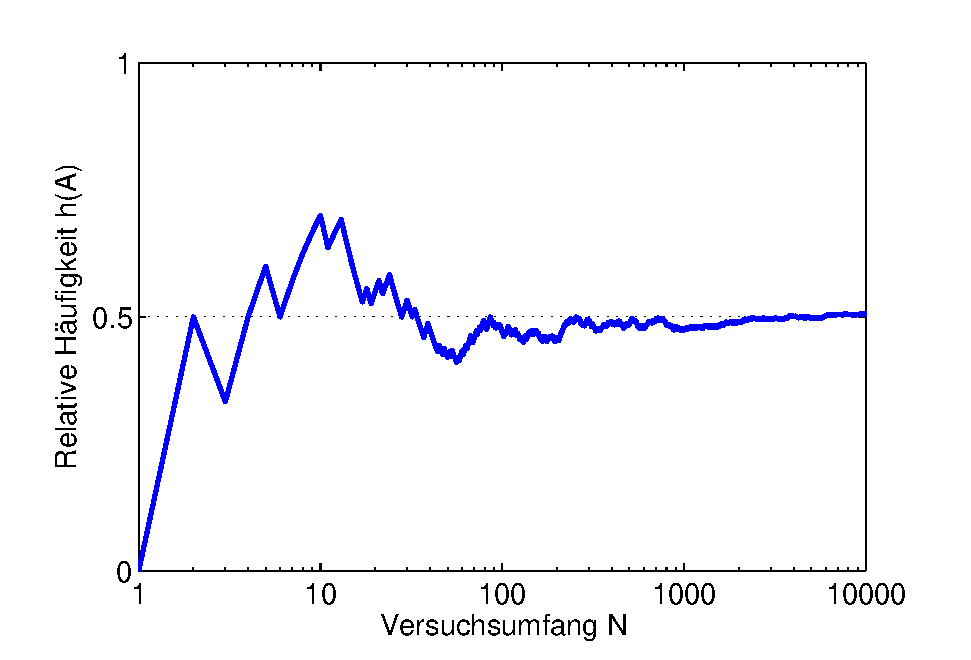
\includegraphics[width=0.5\textwidth]{Kapitel3/Bilder/image9}}
  \caption{Änderung der Integrationsreihenfolge zur Bestimmung der Laplace-Transformierten}
  \label{fig:HerleitungFaltung}
\end{figure}

\noindent Die Integration in Gleichung \eqref{eq:foureightyeight} entspricht der Variante 1. Alternativ kann die in Bild \ref{fig:HerleitungFaltung} die als Variante 2 bezeichnete Integrationsreihenfolge gew\"{a}hlt werden. Dazu muss die Integrationsreihenfolge ge\"{a}ndert werden. Es ergibt sich

\begin{equation}\label{eq:foureightyeight}
\begin{split}
G\left(s\right)\cdot U\left(s\right) & = \int\limits _{0_{-} }^{\infty }g\left(\tau \right)\cdot \int\limits  _{\tau _{-} }^{\infty }u\left(t-\tau \right)\cdot e^{-s\cdot t} \;dt\;d\tau   =\int\limits  _{0_{-} }^{\infty }\int\limits  _{0_{-} }^{t}u\left(t-\tau \right)\cdot g\left(\tau \right)\cdot e^{-s\cdot t} \;d\tau \;dt  \\
& = \int\limits  _{0_{-} }^{\infty }\int\limits  _{0_{-} }^{t}u\left(t-\tau \right)\cdot g\left(\tau \right) \;d\tau \cdot e^{-s\cdot t} \;dt = L\left\{\int\limits _{0_{-} }^{t}u\left(t - \tau \right)\cdot g(\tau) \;d\tau  \right\} \\
& = L\left\{u(t) * g(t)\right\} = L\left\{g(t)*u(t)\right\}
\end{split}
\end{equation}

\noindent Aus der aufwendig auszuwertenden Faltungsoperation im Zeitbereich wird im Laplace-Bereich ein Produkt. Der Berechnung des Ausgangssignals im Zeitbereich 

\begin{equation}\label{eq:foureightynine}
y\left(t\right)=\int\limits _{0_{-} }^{t}u\left(t-\tau \right)\cdot g\left(\tau \right)\;d\tau 
\end{equation}

\noindent entspricht damit im Laplace-Bereich der Ausdruck

\begin{equation}\label{eq:fourninety}
Y\left(s\right)=G\left(s\right)\cdot U\left(s\right)=U\left(s\right)\cdot G\left(s\right)
\end{equation}

\noindent Die Bedeutung und Interpretation der Funktion G(s) ist Gegenstand des Kapitels 5.

\subsubsection{Anfangswertsatz}

\noindent Der Anfangswertsatz erlaubt die Berechnung des Grenzwertes x(0$_{+}$) mithilfe der Laplace-Transformierten X(s). Es gilt

\begin{equation}\label{eq:fourninetyone}
x\left(0_{+} \right)=\lim\limits_{s\to \infty }\; s\cdot X\left(s\right)
\end{equation}

\noindent Der Beweis des Anfangswertsatzes ergibt sich aus der Laplace-Transformierten der Ableitung

\begin{equation}\label{eq:fourninetytwo}
L\left\{\frac{dx}{dt} \right\}=s\cdot X\left(s\right)-x\left(0_{-} \right)
\end{equation}

\noindent Ausführlich kann die Laplace-Transformierte der Ableitung geschrieben werden als 

\begin{equation}\label{eq:fourninetythree}
\int\limits _{0_{-} }^{\infty }\frac{dx}{dt}  \cdot e^{-s\cdot t}\;dt=\int\limits _{0_{-} }^{0_{+} }\frac{dx}{dt}  \cdot e^{-s\cdot t} \;dt+\int\limits _{0_{+} }^{\infty }\frac{dx}{dt}  \cdot e^{-s\cdot t} \;dt=x\left(0_{-} \right)-x\left(0_{+} \right)+\int\limits _{0_{+} }^{\infty }\frac{dx}{dt}  \cdot e^{-s\cdot t} \;dt
\end{equation}

\noindent Für den Grenzwert s $\rightarrow$ $\mathrm{\infty}$ wird das letzte Integral in Gleichung \eqref{eq:fourninetythree} null. 

\begin{equation}\label{eq:fourninetyfour}
\lim\limits_{s\to \infty } \, \, \int\limits _{0_{+} }^{\infty }\frac{dx}{dt}  \cdot e^{-s\cdot t} \; dt=\int\limits _{0_{+} }^{\infty }\frac{dx}{dt}  \cdot \lim\limits_{s\to \infty } \, \, e^{-s\cdot t} \;dt=\int\limits _{0_{+} }^{\infty }\frac{dx}{dt}  \cdot 0\;dt=0
\end{equation}

\noindent Gleichsetzen der Gleichungen \eqref{eq:fourninetytwo} und \eqref{eq:fourninetyfour} führt über 

\begin{equation}\label{eq:fourninetyfive}
x\left(0_{+} \right)-x\left(0_{-} \right)=\;\lim\limits_{s\to \infty } \;s\cdot X\left(s\right)-x\left(0_{-} \right)
\end{equation}

\noindent zu dem Anfangswertsatz

\begin{equation}\label{eq:fourninetysix}
x\left(0_{+} \right)={\mathop{\lim }\limits_{s\to \infty }} \; s\cdot X\left(s\right)
\end{equation}\bigskip

\noindent
\colorbox{lightgray}{%
\arrayrulecolor{white}%
\renewcommand\arraystretch{0.6}%
\begin{tabular}{ wl{16.5cm} }
{\fontfamily{phv}\selectfont{Beispiel: Anfangswertsatz}}
\end{tabular}%
}\bigskip

\noindent Der Anfangswert der Zeitfunktion

\begin{equation}\label{eq:fourninetyseven}
x\left(t\right)=e^{\lambda \cdot t} \cdot \sigma \left(t\right)
\end{equation}

\noindent kann im Laplace-Bereich berechnet werden zu

\begin{equation}\label{eq:fourninetyeight}
x\left(0_{-} \right)=\lim\limits_{s\to \infty}\;s\cdot \frac{1}{s-\lambda } =\lim\limits_{s\to \infty} \;\frac{s}{s-\lambda } =\lim\limits_{s\to \infty} \;\frac{1}{1-\frac{\lambda }{s} } =1
\end{equation}

\noindent Da Ergebnis stimmt mit dem erwarteten Anfangswert üerein.

\subsubsection{Endwertsatz}

\noindent Der Endwertsatz erlaubt die Berechnung des Grenzwertes x($\infty$) mithilfe der Laplace-Transformierten.

\begin{equation}\label{eq:fourninetynine}
\lim \limits_{t\to \infty } \; x\left(t\right)=\lim \limits_{s\to 0} \; s\cdot X\left(s\right)
\end{equation}

\noindent Der Beweis ergibt sich aus der Laplace-Transformierten der Ableitung

\begin{equation}\label{eq:fourhundred}
L\left\{\frac{dx}{dt} \right\}=\int\limits _{0}^{\infty }\frac{dx}{dt}  \cdot e^{-s\cdot t} \;dt=s\cdot X\left(s\right)-x\left(0_{-} \right)
\end{equation}

\noindent Für den Grenzwert s $\rightarrow$ 0 wird die Exponentialfunktion aus dem Integral zu eins. Damit gilt

\begin{equation}\label{eq:fourhundredone}
\lim\limits_{s\to 0} \;\int\limits _{0}^{\infty }\frac{dx}{dt}  \cdot e^{-s\cdot t} \;dt=\int\limits _{0}^{\infty }\frac{dx}{dt}  \;dt=\lim\limits_{t\to \infty } \, \, x\left(t\right)-x\left(0_{-} \right)=\lim\limits_{s\to 0} \;s\cdot X\left(s\right)-x\left(0_{-} \right)
\end{equation}

\noindent Auflösen nach x($\infty$) ergibt

\begin{equation}\label{eq:fourhundredtwo}
\lim\limits_{t\to \infty } \, \, x\left(t\right)=\lim \limits_{s\to 0}\;s\cdot X\left(s\right)
\end{equation}

\noindent Der Endwert x($\infty$) kann jedoch nur berechnet werden, wenn er existiert. In Kapitel 4.3 wird sich zeigen, dass das genau dann der Fall ist, wenn X(s) keine Pole mit Re(s) $\geq$ 0 besitzt.\bigskip

\noindent
\colorbox{lightgray}{%
\arrayrulecolor{white}%
\renewcommand\arraystretch{0.6}%
\begin{tabular}{ wl{16.5cm} }
{\fontfamily{phv}\selectfont{Beispiel: Endwertsatz}}
\end{tabular}%
}\bigskip

\noindent Der Grenzwert der Funktion 

\begin{equation}\label{eq:fourhundredthree}
u_{A} \left(t\right)=5\; V\cdot \left(1-e^{-\frac{t}{R\cdot C} } \right)\cdot \sigma \left(t\right)
\end{equation}

\noindent kann im Laplace-Bereich berechnet werden. Mit der Laplace-Transformierten

\begin{equation}\label{eq:fourhundredfour}
U_{A} \left(s\right)=\frac{5\;V}{s\cdot \left(1+R\cdot C\cdot s\right)} 
\end{equation}

\noindent ergibt sich der Endwert

\begin{equation}\label{eq:fourhundredfive}
u_{A} \left(\infty \right)=\lim\limits_{s\to 0}\; s\cdot \frac{5\; V}{s\cdot \left(1+R\cdot C\cdot s\right)} =\lim\limits_{s\to 0} \; \frac{5\; V}{1+R\cdot C\cdot s} =5\; V
\end{equation}

\subsubsection{Zusammenfassung der Rechenregeln zur Laplace-Transformation}

Tabelle \ref{tab:fourtwo} fasst die wesentlichen Rechenregeln der Laplace-Transformation zusammen. Dabei ist grundsätzlich vorausgesetzt, dass die Zeitfunktion x(t) kausal ist. Mit diesen Rechenregeln können die wichtigsten Korrespondenzen der Laplace-Transformation hergeleitet werden.

\clearpage 

\begin{table}[H]
\setlength{\arrayrulewidth}{.1em}
\caption{Rechenregeln der Laplace-Transformation}
\setlength{\fboxsep}{0pt}%
\colorbox{lightgray}{%
\arrayrulecolor{white}%
\begin{tabular}{| c | c | c |}
\hline
\parbox[c][0.3in][c]{1.9in}{\smallskip\centering\textbf{\fontfamily{phv}\selectfont{Regel}}} & \parbox[c][0.3in][c]{2.2in}{\smallskip\centering\textbf{\fontfamily{phv}\selectfont{Funktion x(t)}}} &
\parbox[c][0.3in][c]{2.2in}{\smallskip\centering\textbf{\fontfamily{phv}\selectfont{Laplace-Transformierte X(s)}}}\\ \hline


\parbox[c][0.5in][c]{1.9in}{\centering{\fontfamily{phv}\selectfont{Linearität}}} & 
\parbox[c][0.5in][c]{2.2in}{\centering{$\nu _{1} \cdot x_{1} \left(t\right)+\nu _{2} \cdot x_{2} \left(t\right)$}} &
\parbox[c][0.5in][c]{2.2in}{\centering{$\nu _{1} \cdot X_{1} \left(s\right)+\nu _{2} \cdot X_{2} \left(s\right)$}}\\
\hline

\parbox[c][0.5in][c]{1.9in}{\centering{\fontfamily{phv}\selectfont{Zeitverschiebung nach rechts}}} & 
\parbox[c][0.5in][c]{2.2in}{\centering{$x\left(t-t_{0} \right)$}} &
\parbox[c][0.5in][c]{2.2in}{\centering{$e^{-s\cdot t_{0} } \cdot X\left(s\right)$}}\\
\hline

\parbox[c][0.5in][c]{1.9in}{\centering{\fontfamily{phv}\selectfont{Modulation}}} & 
\parbox[c][0.5in][c]{2.2in}{\centering{$e^{\lambda \cdot t} \cdot x\left(t\right)$}} &
\parbox[c][0.5in][c]{2.2in}{\centering{ $X\left(s-\lambda \right)$}}\\
\hline

\parbox[c][0.5in][c]{1.9in}{\centering{\fontfamily{phv}\selectfont{Lineare Gewichtung }}} & 
\parbox[c][0.5in][c]{2.2in}{\centering{$t\cdot x\left(t\right)$}} &
\parbox[c][0.5in][c]{2.2in}{\centering{$-\frac{dX}{ds} $}}\\
\hline

\parbox[c][0.5in][c]{1.9in}{\centering{\fontfamily{phv}\selectfont{Skalierung}}} & 
\parbox[c][0.5in][c]{2.2in}{\centering{$x\left(c\cdot t\right)$ }} &
\parbox[c][0.5in][c]{2.2in}{\centering{$\frac{1}{c} \cdot X\left(\frac{s}{c} \right)$ }}\\
\hline

\parbox[c][0.5in][c]{1.9in}{\centering{\fontfamily{phv}\selectfont{Skalierung}}} & 
\parbox[c][0.5in][c]{2.2in}{\centering{$\frac{1}{c} \cdot x\left(\frac{t}{c} \right)$ }} &
\parbox[c][0.5in][c]{2.2in}{\centering{$X\left(c\cdot s\right)$}}\\
\hline

\parbox[c][0.5in][c]{1.9in}{\centering{\fontfamily{phv}\selectfont{Integration}}} & 
\parbox[c][0.5in][c]{2.2in}{\centering{ $\int _{0}^{t}x\left(\tau \right){\rm \; }d\tau  $}} &
\parbox[c][0.5in][c]{2.2in}{\centering{$\frac{1}{s} \cdot X\left(s\right)$}}\\
\hline

\parbox[c][0.5in][c]{1.9in}{\centering{\fontfamily{phv}\selectfont{Ableitung}}} & 
\parbox[c][0.5in][c]{2.2in}{\centering{$\frac{dx}{dt} $ }} &
\parbox[c][0.5in][c]{2.2in}{\centering{$s\cdot X\left(s\right)-x\left(0_{-} \right)$ }}\\
\hline

\parbox[c][0.8in][c]{1.9in}{\centering{\fontfamily{phv}\selectfont{n-fache Ableitung}}} & 
\parbox[c][0.8in][c]{2.2in}{\centering{ $\frac{d^{n} x}{dt^{n} } $}} &
\parbox[c][0.8in][c]{2.2in}{\centering{$s^{n} \cdot X\left(s\right)-s^{n-1} \cdot x\left(0_{-} \right)-...-\left. \frac{d^{n-1} x}{dt^{n-1} } \right|_{t=0_{-} } $}}\\
\hline

\parbox[c][0.5in][c]{1.9in}{\centering{\fontfamily{phv}\selectfont{Multiplikation}}} & 
\parbox[c][0.5in][c]{2.2in}{\centering{$x\left(t\right)\cdot w\left(t\right)$ }} &
\parbox[c][0.5in][c]{2.2in}{\centering{$X\left(s\right)*W\left(s\right)$}}\\
\hline

\parbox[c][0.5in][c]{1.9in}{\centering{\fontfamily{phv}\selectfont{Faltung}}} & 
\parbox[c][0.5in][c]{2.2in}{\centering{$g\left(t\right)*x\left(t\right)$ }} &
\parbox[c][0.5in][c]{2.2in}{\centering{$G\left(s\right)\cdot X\left(s\right)$}}\\
\hline

\parbox[c][0.5in][c]{1.9in}{\centering{\fontfamily{phv}\selectfont{Anfangswert}}} & 
\parbox[c][0.5in][c]{2.2in}{\centering{${\mathop{\lim }\limits_{t\to 0_{+} }} \, \, x\left(t\right)$ }} &
\parbox[c][0.5in][c]{2.2in}{\centering{${\mathop{\lim }\limits_{s\to \infty }} \, \, s\cdot X\left(s\right)$}}\\
\hline

\parbox[c][0.5in][c]{1.9in}{\centering{\fontfamily{phv}\selectfont{Endwert}}} & 
\parbox[c][0.5in][c]{2.2in}{\centering{${\mathop{\lim }\limits_{t\to \infty }} \, \, x\left(t\right)$ }} &
\parbox[c][0.5in][c]{2.2in}{\centering{${\mathop{\lim }\limits_{s\to 0}} \, \, s\cdot X\left(s\right)$}}\\
\hline
\end{tabular}%
}
\label{tab:fourtwo}
\end{table}

\subsubsection{Korrespondenzen der Laplace-Transformation}

\noindent Die Rechenregeln zur Laplace-Transformation erlauben die Berechnung weiterer Korrespondenzen.
Tabelle \ref{tab:fourthree} und Tabelle \ref{tab:fourfour} stellen wichtige Korrespondenzen der Laplace-Transformation zusammen.
Die Korrespondenztafel ermöglicht die schnelle Angabe von Laplace-Transformierten der aufgeführten Zeitfunktionen. Um die Korrespondenztafeln anwenden zu können, muss die vorliegende Zeitfunktion gegebenenfalls durch Zerlegung nach dem Linearitätsprinzip, Verschiebung im Zeitbereich oder Dehnung/Stauchung mit dem Ähnlichkeitssatz umgeformt werden.

\clearpage

\begin{table}[H]
\setlength{\arrayrulewidth}{.1em}
\caption{Korrespondenzen der Laplace-Transformation (1/2)}
\setlength{\fboxsep}{0pt}%
\colorbox{lightgray}{%
\arrayrulecolor{white}%
\begin{tabular}{| c | c | c | c |}
\hline
\parbox[c][0.3in][c]{0.3in}{\smallskip\centering\textbf{\fontfamily{phv}\selectfont{Nr}}} &
\parbox[c][0.5in][c]{2.4in}{\smallskip\centering\textbf{\fontfamily{phv}\selectfont{Zeitfunktion x(t)}}} & \parbox[c][0.5in][c]{1.2in}{\smallskip\centering\textbf{\fontfamily{phv}\selectfont{Konvergenz-\\bereich}}} &
\parbox[c][0.5in][c]{2.4in}{\smallskip\centering\textbf{\fontfamily{phv}\selectfont{Laplace-Transformierte X(s)}}}\\ \hline

\parbox[c][0.5in][c]{0.3in}{\centering{1}} &
\parbox[c][0.5in][c]{2.4in}{\centering{$\delta \left(t\right)$}} & 
\parbox[c][0.5in][c]{1.2in}{\centering{$s \in C$}} & 
\parbox[c][0.5in][c]{2.4in}{\centering{1}}\\
\hline

\parbox[c][0.5in][c]{0.3in}{\centering{2}} &
\parbox[c][0.5in][c]{2.4in}{\centering{$\delta \left(t-t_{0} \right)$}} & 
\parbox[c][0.5in][c]{1.2in}{\centering{$s \in C$}} & 
\parbox[c][0.5in][c]{2.4in}{\centering{$e^{-t_{0} \cdot s} $}}\\
\hline

\parbox[c][0.5in][c]{0.3in}{\centering{3}} &
\parbox[c][0.5in][c]{2.4in}{\centering{$1\cdot \sigma \left(t\right)$}} & 
\parbox[c][0.5in][c]{1.2in}{\centering{Re$\left(s\right)>0$}} & 
\parbox[c][0.5in][c]{2.4in}{\centering{$\frac{1}{s} $}}\\
\hline

\parbox[c][0.5in][c]{0.3in}{\centering{4}} &
\parbox[c][0.5in][c]{2.4in}{\centering{$t\cdot \sigma \left(t\right)$}} & 
\parbox[c][0.5in][c]{1.2in}{\centering{Re$\left(s\right)>0$}} & 
\parbox[c][0.5in][c]{2.4in}{\centering{$\frac{1}{s^{2} } $}}\\
\hline

\parbox[c][0.5in][c]{0.3in}{\centering{5}} &
\parbox[c][0.5in][c]{2.4in}{\centering{$\frac{1}{2} \cdot t^{2} \cdot \sigma \left(t\right)$}} & 
\parbox[c][0.5in][c]{1.2in}{\centering{Re$\left(s\right)>0$}} & 
\parbox[c][0.5in][c]{2.4in}{\centering{$\frac{1}{s^{3} } $}}\\
\hline

\parbox[c][0.5in][c]{0.3in}{\centering{6}} &
\parbox[c][0.5in][c]{2.4in}{\centering{$\frac{1}{n!} \cdot t^{n} \cdot \sigma \left(t\right)$}} & 
\parbox[c][0.5in][c]{1.2in}{\centering{Re$\left(s\right)>0$}} & 
\parbox[c][0.5in][c]{2.4in}{\centering{$\frac{1}{s^{n+1}}$ für n$\;$=$\;$ 0,$\;$1, $\;$ ...}}\\
\hline

\parbox[c][0.5in][c]{0.3in}{\centering{7}} &
\parbox[c][0.5in][c]{2.4in}{\centering{$e^{\lambda \cdot t} \cdot \sigma \left(t\right)$}} & 
\parbox[c][0.5in][c]{1.2in}{\centering{Re$\left(s\right)>$Re$\left(\lambda \right)$}} & 
\parbox[c][0.5in][c]{2.4in}{\centering{$\frac{1}{s-\lambda}$}}\\
\hline

\parbox[c][0.5in][c]{0.3in}{\centering{8}} &
\parbox[c][0.5in][c]{2.4in}{\centering{$t\cdot e^{\lambda \cdot t} \cdot \sigma \left(t\right)$}} & 
\parbox[c][0.5in][c]{1.2in}{\centering{Re$\left(s\right)>$Re$\left(\lambda \right)$}} & 
\parbox[c][0.5in][c]{2.4in}{\centering{$\frac{1}{\left(s-\lambda \right)^{2} } $}}\\
\hline

\parbox[c][0.5in][c]{0.3in}{\centering{9}} &
\parbox[c][0.5in][c]{2.4in}{\centering{$\frac{1}{n!} \cdot t^{n} \cdot e^{\lambda \cdot t} \cdot \sigma \left(t\right)$}} & 
\parbox[c][0.5in][c]{1.2in}{\centering{Re$\left(s\right)>$Re$\left(\lambda \right)$}} & 
\parbox[c][0.5in][c]{2.4in}{\centering{$\frac{1}{\left(s-\lambda \right)^{n+1} }$ für n$\;$=$\;$ 0,$\;$1, $\;$ ...}}\\
\hline
 
\parbox[c][0.5in][c]{0.3in}{\centering{10}} &
\parbox[c][0.5in][c]{2.4in}{\centering{$\frac{1}{T} \cdot e^{-\frac{t}{T} } \cdot \sigma \left(t\right)$}} & 
\parbox[c][0.5in][c]{1.2in}{\centering{Re$\left(s\right)>-\frac{1}{T} $}} & 
\parbox[c][0.5in][c]{2.4in}{\centering{$\frac{1}{1+T\cdot s} $}}\\
\hline

\parbox[c][0.5in][c]{0.3in}{\centering{11}} &
\parbox[c][0.5in][c]{2.4in}{\centering{$\delta \left(t\right)-\frac{1}{T} \cdot e^{-\frac{t}{T} } \cdot \sigma \left(t\right)$}} & 
\parbox[c][0.5in][c]{1.2in}{\centering{Re$\left(s\right)>-\frac{1}{T} $}} & 
\parbox[c][0.5in][c]{2.4in}{\centering{$\frac{T\cdot s}{1+T\cdot s} $}}\\
\hline

\parbox[c][0.5in][c]{0.3in}{\centering{12}} &
\parbox[c][0.5in][c]{2.4in}{\centering{$\left(1-e^{-\frac{t}{T} } \right)\cdot \sigma \left(t\right)$}} & 
\parbox[c][0.5in][c]{1.2in}{\centering{Re$\left(s\right)>0$}} & 
\parbox[c][0.5in][c]{2.4in}{\centering{$\frac{1}{s\cdot \left(1+T\cdot s\right)} $}}\\
\hline

\parbox[c][0.5in][c]{0.3in}{\centering{13}} &
\parbox[c][0.5in][c]{2.4in}{\centering{$\frac{t}{T^{2} } \cdot e^{-\frac{t}{T} } \cdot \sigma \left(t\right)$}} & 
\parbox[c][0.5in][c]{1.2in}{\centering{Re$\left(s\right)>-\frac{1}{T} $}} & 
\parbox[c][0.5in][c]{2.4in}{\centering{$\frac{1}{\left(1+T\cdot s\right)^{2} }$}}\\
\hline

\parbox[c][0.5in][c]{0.3in}{\centering{14}} &
\parbox[c][0.5in][c]{2.4in}{\centering{$\left(t-T\cdot \left(1-e^{-\frac{t}{T} } \right)\right)\cdot \sigma \left(t\right)$}} & 
\parbox[c][0.5in][c]{1.2in}{\centering{Re$\left(s\right)>0$}} & 
\parbox[c][0.5in][c]{2.4in}{\centering{$\frac{1}{s^{2} \cdot \left(1+T\cdot s\right)}$}}\\
\hline

\end{tabular}%
}
\label{tab:fourthree}
\end{table}

\clearpage

\begin{table}[H]
\setlength{\arrayrulewidth}{.1em}
\caption{Korrespondenzen der Laplace-Transformation (2/2)}
\setlength{\fboxsep}{0pt}%
\colorbox{lightgray}{%
\arrayrulecolor{white}%
\begin{tabular}{| c | c | c | c |}
\hline
\parbox[c][0.3in][c]{0.3in}{\smallskip\centering\textbf{\fontfamily{phv}\selectfont{Nr}}} &
\parbox[c][0.5in][c]{2.4in}{\smallskip\centering\textbf{\fontfamily{phv}\selectfont{Zeitfunktion x(t)}}} & \parbox[c][0.5in][c]{1.2in}{\smallskip\centering\textbf{\fontfamily{phv}\selectfont{Konvergenz-\\bereich}}} &
\parbox[c][0.5in][c]{2.4in}{\smallskip\centering\textbf{\fontfamily{phv}\selectfont{Laplace-Transformierte X(s)}}}\\ \hline

\parbox[c][0.5in][c]{0.3in}{\centering{15}} &
\parbox[c][0.5in][c]{2.4in}{\centering{$\sin \left(\omega _{0} \cdot t\right)\cdot \sigma \left(t\right)$}} & 
\parbox[c][0.5in][c]{1.2in}{\centering{Re$\left(s\right)>0$}} & 
\parbox[c][0.5in][c]{2.4in}{\centering{$\frac{\omega _{0} }{s^{2} +\omega _{0}^{2} } $}}\\
\hline

\parbox[c][0.5in][c]{0.3in}{\centering{16}} &
\parbox[c][0.5in][c]{2.4in}{\centering{$\cos \left(\omega _{0} \cdot t\right)\cdot \sigma \left(t\right)$}} & 
\parbox[c][0.5in][c]{1.2in}{\centering{Re$\left(s\right)>0$}} & 
\parbox[c][0.5in][c]{2.4in}{\centering{$\frac{s}{s^{2} +\omega _{0}^{2} } $}}\\
\hline

\parbox[c][0.5in][c]{0.3in}{\centering{17}} &
\parbox[c][0.5in][c]{2.4in}{\centering{$\sinh \left(\lambda \cdot t\right)\cdot \sigma \left(t\right)$}} & 
\parbox[c][0.5in][c]{1.2in}{\centering{Re$\left(s\right)>\lambda$}} & 
\parbox[c][0.5in][c]{2.4in}{\centering{$\frac{\lambda }{s^{2} -\lambda ^{2} } $}}\\
\hline

\parbox[c][0.5in][c]{0.3in}{\centering{18}} &
\parbox[c][0.5in][c]{2.4in}{\centering{$\cosh \left(\lambda \cdot t\right)\cdot \sigma \left(t\right)$}} & 
\parbox[c][0.5in][c]{1.2in}{\centering{Re$\left(s\right)>\lambda$}} & 
\parbox[c][0.5in][c]{2.4in}{\centering{$\frac{s}{s^{2} -\lambda ^{2} } $}}\\
\hline

\parbox[c][0.5in][c]{0.3in}{\centering{19}} &
\parbox[c][0.5in][c]{2.4in}{\centering{$\frac{1}{2} \cdot t^{2} \cdot \sigma \left(t\right)$}} & 
\parbox[c][0.5in][c]{1.2in}{\centering{Re$\left(s\right)>\delta _{0}$}} & 
\parbox[c][0.5in][c]{2.4in}{\centering{$\frac{1}{s^{3} } $}}\\
\hline

\parbox[c][0.5in][c]{0.3in}{\centering{20}} &
\parbox[c][0.5in][c]{2.4in}{\centering{ $\frac{1}{\omega _{0} } \cdot e^{\delta _{0} \cdot t} \cdot \sin \left(\omega _{0} \cdot t\right)\cdot \sigma \left(t\right)$}} & 
\parbox[c][0.5in][c]{1.2in}{\centering{Re$\left(s\right)>\delta _{0}$}} & 
\parbox[c][0.5in][c]{2.4in}{\centering{$\frac{1}{\left(s-\delta _{0} \right)^{2} +\omega _{0}^{2} } $}}\\
\hline

\parbox[c][0.6in][c]{0.3in}{\centering{21}} &
\parbox[c][0.6in][c]{2.4in}{\centering{$\frac{t}{2\cdot \omega _{0} } \cdot \sin \left(\omega _{0} \cdot t\right)\cdot \sigma \left(t\right)$}} & 
\parbox[c][0.6in][c]{1.2in}{\centering{Re$\left(s\right)>0$}} & 
\parbox[c][0.6in][c]{2.4in}{\centering{$\frac{s}{\left(s^{2} +\omega _{0}^{2} \right)^{2} } $}}\\
\hline

\parbox[c][0.6in][c]{0.3in}{\centering{22}} &
\parbox[c][0.6in][c]{2.4in}{\centering{$t\cdot \cos \left(\omega _{0} \cdot t\right)\cdot \sigma \left(t\right)$}} & 
\parbox[c][0.6in][c]{1.2in}{\centering{Re$\left(s\right)>0$}} & 
\parbox[c][0.6in][c]{2.4in}{\centering{$\frac{s^{2} -\omega _{0}^{2} }{\left(s^{2} +\omega _{0}^{2} \right)^{2} } $}}\\
\hline

\parbox[c][0.6in][c]{0.3in}{\centering{23}} &
\parbox[c][0.6in][c]{2.4in}{\centering{$\frac{t}{2\cdot \omega _{0} } \cdot e^{\delta _{0} \cdot t} \sin \left(\omega _{0} \cdot t\right)\cdot \sigma \left(t\right)$}} & 
\parbox[c][0.6in][c]{1.2in}{\centering{Re$\left(s\right)>\delta _{0}$}} & 
\parbox[c][0.6in][c]{2.4in}{\centering{$\frac{s-\delta _{0} }{\left(s^{2} -2\cdot \delta _{0} \cdot s+\delta _{0}^{2} +\omega _{0}^{2} \right)^{2} } $}}\\
\hline
 
\parbox[c][0.6in][c]{0.3in}{\centering{24}} &
\parbox[c][0.6in][c]{2.4in}{\centering{$t\cdot e^{\delta _{0} \cdot t} \cos \left(\omega _{0} \cdot t\right)\cdot \sigma \left(t\right)$}} & 
\parbox[c][0.6in][c]{1.2in}{\centering{Re$\left(s\right)>\delta _{0}$}} & 
\parbox[c][0.6in][c]{2.4in}{\centering{$\frac{s^{2} -2\cdot \delta _{0} \cdot s+\delta _{0}^{2} -\omega _{0} }{\left(s^{2} -2\cdot \delta _{0} \cdot s+\delta _{0}^{2} +\omega _{0}^{2} \right)^{2} } $}}\\
\hline

\parbox[c][0.5in][c]{0.3in}{\centering{25}} &
\parbox[c][0.5in][c]{2.4in}{\centering{$\frac{1}{\sqrt{\pi \cdot t} } \cdot \sigma \left(t\right)$}} & 
\parbox[c][0.5in][c]{1.2in}{\centering{Re$\left(s\right)>\delta _{0}$}} & 
\parbox[c][0.5in][c]{2.4in}{\centering{$\frac{1}{\sqrt{s} } $}}\\
\hline

\parbox[c][0.5in][c]{0.3in}{\centering{26}} &
\parbox[c][0.5in][c]{2.4in}{\centering{$\frac{e^{\delta _{0} \cdot t} }{\sqrt{\pi \cdot t} } \cdot \sigma \left(t\right)$}} & 
\parbox[c][0.5in][c]{1.2in}{\centering{Re$\left(s\right)>0$}} & 
\parbox[c][0.5in][c]{2.4in}{\centering{$\frac{1}{\sqrt{s-\delta _{0} } } $}}\\
\hline

\parbox[c][0.5in][c]{0.3in}{\centering{27}} &
\parbox[c][0.5in][c]{2.4in}{\centering{$2\cdot \sqrt{\frac{t}{\pi } } \cdot \sigma \left(t\right)$}} & 
\parbox[c][0.5in][c]{1.2in}{\centering{Re$\left(s\right)>\delta _{0}$}} & 
\parbox[c][0.5in][c]{2.4in}{\centering{$\frac{1}{s\cdot \sqrt{s} } $}}\\
\hline

\end{tabular}%
}
\label{tab:fourfour}
\end{table}

\clearpage

\subsection{Rücktransformation}

\noindent Das Beispiel in Abschnitt \ref{fourtwoseven} zeigt, dass für den Einsatz der Laplace-Transformation bei der Lösung linearer Differentialgleichungen eine Rücktransformation erforderlich ist. Sie lässt sich zum einen als mathematische Umkehrformel angeben, was in der Praxis jedoch aufwendig und wenig gebräuchlich
ist.\medskip

\noindent In dem Beispiel des Abschnitts \ref{fourtwoseven} wird die Funktion im Laplace-Bereich so zerlegt, dass bekannte Korrespondenzen aus der Korrespondenztabelle eingesetzt werden können. Dieses Vorgehen erfordert eine Partialbruchzerlegung der Laplace-Transformierten. Das Vorgehen zur Rücktransformation über eine Partialbruchzerlegung wird nach der Vorstellung der Umkehrformel zur Laplace-Transformation weiter vertieft.

\subsubsection{Definition der inversen Laplace-Transformation}\label{fourthreeone}

\noindent Die Umkehrformel zur Laplace-Transformation lautet [Foel11]:

\begin{equation}\label{eq:fourhundredsix}
x\left(t\right)=\frac{1}{2\cdot \pi \cdot j} \cdot \int\limits _{\delta -j\cdot \infty }^{\delta +j\cdot \infty }X\left(s\right) \cdot e^{s\cdot t}\; ds=L^{-1} \left\{X\left(s\right)\right\}
\end{equation}

\noindent Die Rücktransformation wird als inverse Laplace-Transformation bezeichnet. Das eingeführte Hantelsymbol kennzeichnet eine Korrespondenz und wird deshalb für Hin- und Rücktransformation verwendet. 

\begin{equation}\label{eq:fourhundredseven}
X\left(s\right)\bullet -\circ x\left(t\right)
\end{equation}

\noindent Der Einsatz der Umkehrformel ist aufwendig und wird deshalb mithilfe der Partialbruchzerlegung und bekannten Korrespondenzen umgangen. Die Umkehrformel kann jedoch zur Herleitung von Rechenregeln zur Laplace-Transformation nützlich sein, was an der Faltungsoperation im Laplace-Bereich aufgezeigt wird. Die Laplace-Transformierte für das Produkt zweier Zeitfunktionen ist definiert als

\begin{equation}\label{eq:fourhundredeight}
L\left\{x\left(t\right)\cdot w\left(t\right)\right\}=\int\limits _{0}^{\infty }x\left(t\right)\cdot w\left(t\right)\cdot e^{-s\cdot t} \;dt
\end{equation}

\noindent Die Zeitfunktion x(t) kann über die inverse Laplace-Transformierte ausgedrückt werden.

\begin{equation}\label{eq:fourhundrednine}
L\left\{x\left(t\right)\cdot w\left(t\right)\right\}=\int\limits _{0}^{\infty }x\left(t\right)\cdot w\left(t\right)\cdot e^{-s\cdot t} \;dt =\int\limits _{0}^{\infty }\frac{1}{2\cdot \pi \cdot j} \cdot \int\limits _{\delta -j\infty }^{\delta +j\infty }X\left(\upsilon \right) \cdot e^{\upsilon \cdot t} \;d\upsilon \cdot w\left(t\right)\cdot e^{-s\cdot t} \;dt 
\end{equation}

\noindent Ausklammern des Vorfaktors und Tauschen der Integrationsreihenfolge führt zu

\begin{equation}\label{eq:fourhundredten}
\begin{split}
L\left\{x\left(t\right)\cdot w\left(t\right)\right\} & = {\frac{1}{2\cdot \pi \cdot j} \cdot \int\limits _{\delta -j\infty }^{\delta +j\infty }X\left(\upsilon \right) \cdot \int\limits _{0}^{\infty }w\left(t\right)\cdot e^{-(s-\upsilon )\cdot t} \;  dt\; d\upsilon } \\ 
& = {\frac{1}{2\cdot \pi \cdot j} \cdot \int\limits _{\delta -j\infty }^{\delta +j\infty }X\left(\upsilon \right) \cdot W\left(s-\upsilon \right)\; d\upsilon =X\left(s\right)*W\left(s\right)}
\end{split}
\end{equation}

\noindent Die Laplace-Transformierte des Produktes zweier Zeitfunktionen entspricht demnach der komplexen Faltung der beiden Funktionen im Laplace-Bereich.


\subsubsection{Rücktransformation über Partialbruchzerlegung}

\noindent In den bisher behandelten Beispielen und Rechenregeln sind immer gebrochen rationale Funktionen der Form 

\begin{equation}\label{eq:fourhundredeleven}
X\left(s\right)=\frac{B\left(s\right)}{A\left(s\right)} =\frac{\sum _{m=0}^{M}b_{m} \cdot s^{m}  }{\sum _{n=0}^{N}a_{n} \cdot s^{n}  } =\frac{b_{M} }{a_{N} } \cdot \frac{\prod _{m=1}^{M}\left(s-\beta _{m} \right) }{\prod _{n=1}^{N}\left(s-\alpha _{n} \right) } 
\end{equation}

\noindent entstanden. Da sich die Laplace-Transformation auf kausale Signale beschränkt, ist der Zählergrad maximal so gro{\ss} wie der Nennergrad M $\leq$ N. Die Koeffizienten a${}_{n}$ und b${}_{m}$ sind reelle Koeffizienten. Damit sind die Pol- und Nullstellen von X(s) entweder reell oder konjugiert komplex.

\noindent Die gebrochen rationalen Funktionen X(s) lassen sich in seltenen Fällen direkt über eine bekannte Korrespondenz zurücktransformieren. Im Allgemeinen ist eine Zerlegung der Funktion mit der Partialbruchzerlegung notwendig. Nach der Partialbruchzerlegung liegen einzelne Partialbrüche vor, die auf bekannte Korrespondenzen zurückgeführt werden können.\bigskip

{\fontfamily{phv}\selectfont
\noindent\textbf{Vorbereitung der Partialbruchzerlegung falls Zählergrad M gleich Nennergrad N}}\smallskip

\noindent Für den Fall, dass Zählergrad M gleich Nennergrad N gleich gro{\ss} sind (M = N), muss vor der Partialbruchzerlegung eine Polynomdivision durchgeführt werden. Dadurch entsteht ein konstanter Summand 

\begin{equation}\label{eq:fourhundredtwelve}
X_{0} =\frac{b_{M} }{a_{N} } 
\end{equation}

\noindent Da die inverse Laplace-Transformierte von einer Konstanten die Impulsfunktion $\delta$(t) ist, entspricht diesem Summand ein Impuls zum Zeitpunkt t = 0

\begin{equation}\label{eq:fourhundredthirteen}
x_{0} \left(t\right)=\frac{b_{M} }{a_{N} } \cdot \delta \left(t\right)
\end{equation}\bigskip

\noindent
\colorbox{lightgray}{%
\arrayrulecolor{white}%
\renewcommand\arraystretch{0.6}%
\begin{tabular}{ wl{16.5cm} }
{\fontfamily{phv}\selectfont{Beispiel: Zählergrad gleich Nennergrad} }
\end{tabular}%
}\bigskip

\noindent Die Laplace-Transformierte X(s) soll in den Zeitbereich zurück transformiert werden. Da der Zählergrad genauso gro{\ss} ist wie der Nennergrad, wird eine Polynomdivision durchgeführt.

\begin{equation}\label{eq:fourhundredfourteen}
X\left(s\right)=\frac{2\cdot s-3}{s-3} =2+\frac{3}{s-3}
\end{equation}

\noindent Damit kann die Funktion im Zeitbereich mit der Korrespondenztafel bestimmt werden zu

\begin{equation}\label{eq:fourhundredfifteen}
x\left(t\right)=2\cdot \delta \left(t\right)+3\cdot e^{3\cdot t} \cdot \sigma \left(t\right)
\end{equation}\bigskip

{\fontfamily{phv}\selectfont
\noindent\textbf{Partialbruchzerlegung für einfache Pole $\alpha$}}\smallskip

\noindent Besitzt die Laplace-Transformierte X(s) nur einfache Pole $\alpha_{n}$, kann Sie mithilfe der Partialbruchzerlegung dargestellt werden als

\begin{equation}\label{eq:fourhundredsixteen}
X\left(s\right)=\frac{1}{a_{N} } \cdot \frac{\sum _{M=0}^{M}b_{m} \cdot s^{m}  }{\prod _{n=1}^{N}\left(s-\alpha _{n} \right) } =\sum _{n=1}^{N}\frac{A_{n} }{s-\alpha _{n} } 
\end{equation}

\noindent Die Koeffizienten A$_{n}$ der einzelnen Partialbrüche können auf unterschiedliche Arten berechnet werden:

\begin{itemize}
\item  Ausmultiplizieren\\
Die Gleichung wird mit den Linearfaktoren des Nenners multipliziert. Anschlie{\ss}end werden die Polstellen eingesetzt, und es ergibt sich ein Gleichungssystem für die Koeffizient A$_{n}$. 

\item  Residuensatz\\
Die einzelnen Koeffizienten werden über den Residuensatz berechnet \\
\begin{equation}\label{eq:fourhundredseventeen}
A_{n} =\left. \left(X\left(s\right)\cdot \left(s-\alpha _{n} \right)\right)\right|_{s=\alpha _{n} } 
\end{equation}
\end{itemize}

\noindent Jeder einzelne Partialbruch hat die Form 

\begin{equation}\label{eq:fourhundredeighteen}
X_{n} \left(s\right)=\frac{A_{n} }{s-\alpha _{n} }
\end{equation}

\noindent Im Zeitbereich ergibt sich damit für jeden Partialbruch eine Exponentialfunktion.

\begin{equation}\label{eq:fourhundrednineteen}
x_{n} \left(t\right)=L^{-1} \left\{\frac{A_{n} }{s-\alpha _{n} } \right\}=A_{n} \cdot e^{\alpha _{n} \cdot t} \cdot \sigma \left(t\right)
\end{equation}

Die Summe der Partialbrüche aus Gleichung \eqref{eq:fourhundredsixteen} entspricht deshalb im Zeitbereich der Summe

\begin{equation}\label{eq:fourhundredtwenty}
{\rm L}^{-1} \left\{\sum _{n=1}^{N}\frac{A_{n} }{s-\alpha _{n} }  \right\}=\sum _{n=1}^{N}A_{n} \cdot e^{\alpha _{n} \cdot t} \cdot \sigma \left(t\right) 
\end{equation}\bigskip

\noindent
\colorbox{lightgray}{%
\arrayrulecolor{white}%
\renewcommand\arraystretch{0.6}%
\begin{tabular}{ wl{16.5cm} }
{\fontfamily{phv}\selectfont{Beispiel: Partialbruchzerlegung für einfache Pole $\alpha_{n}$} }
\end{tabular}%
}\bigskip

\noindent Die Laplace-Transformierte X(s) soll in den Zeitbereich zurücktransformiert werden. Ihr Zählergrad ist kleiner als der Nennergrad, und sie hat zwei einfache Pole. 

\begin{equation}\label{eq:fourhundredstwentyone}
X\left(s\right)=\frac{s}{s^{2} +3\cdot s+2} =\frac{s}{\left(s+1\right)\cdot \left(s+2\right)} =\frac{A_{1} }{s+1} +\frac{A_{2} }{s+2} 
\end{equation}

\noindent Ausmultiplizieren der Gleichung führt zu

\begin{equation}\label{eq:fourhundredstwentytwo}
s=A_{1} \cdot \left(s+2\right)+A_{2} \cdot \left(s+1\right)
\end{equation}

\noindent Einsetzen der Polstellen $\alpha_{1}$= - 1 und $\alpha_{2}$= - 2 führt zu 

\begin{equation}\label{eq:fourhundredstwentythree}
A_{1} =-1
\end{equation}

\noindent und

\begin{equation}\label{eq:fourhundredstwentyfour}
A_{2} =2
\end{equation}

\noindent Alternativ hätte der Residuensatz ergeben

\begin{equation}\label{eq:fourhundredstwentyfive}
A_{1} =\left. \left(\frac{s}{\left(s+1\right)\cdot \left(s+2\right)} \cdot \left(s+1\right)\right)\right|_{s=-1} =\left. \left(\frac{s}{s+2} \right)\right|_{s=-1} =\frac{-1}{-1+2} =-1
\end{equation}

\noindent und

\begin{equation}\label{eq:fourhundredstwentysix}
A_{2} =\left. \left(\frac{s}{\left(s+1\right)\cdot \left(s+2\right)} \cdot \left(s+2\right)\right)\right|_{s=-2} =\left. \left(\frac{s}{s+1} \right)\right|_{s=-2} =\frac{-2}{-2+1} =2
\end{equation}

\noindent Sind die Koeffizienten der Partialbrüche bestimmt, kann die Laplace-Transformierte mit den bekannten Korrespondenzen in den Zeitbereich zurücktransformiert werden.

\begin{equation}\label{eq:fourhundredstwentyseven}
X\left(s\right)=\frac{-1}{s+1} +\frac{2}{s+2} 
\end{equation}

\noindent Es ergibt sich die Funktion

\begin{equation}\label{eq:fourhundredstwentyeight}
x\left(t\right)=-1\cdot e^{-1\cdot t} \cdot \sigma \left(t\right)+2\cdot e^{-2\cdot t} \cdot \sigma \left(t\right)
\end{equation}
\clearpage

{\fontfamily{phv}\selectfont
\noindent\textbf{Partialbruchzerlegung für konjugiert komplexe Polpaare}}\smallskip

\noindent Bei komplexen Polen gelten dieselben Regeln und Formeln wie bei den reellen Polen. Die Koeffizienten können mit denselben Verfahren bestimmt werden. Die Rücktransformation kann jedoch durch einen modifizierten Ansatz zur Partialbruchzerlegung vereinfacht werden. Dabei wird die Eigenschaft genutzt, dass bei Laplace-Transformierten mit reellen Koeffizienten a$_{n}$ und b$_{n}$ komplexe Pole $\alpha_{n}$ immer als konjugiert komplexe Polpaare auftreten. 

\begin{equation}\label{eq:fourhundredstwentynine}
\alpha _{n} =\delta _{n} \pm j\cdot \omega _{n}
\end{equation}

\noindent Au{\ss}erdem sind in diesem Fall die Koeffizienten A${}_{n}$ der Partialbr\"{u}che konjugiert komplex zueinander.

\begin{equation}\label{eq:fourhundredsthirty}
X_{n} \left(s\right)=\frac{A_{n} }{s-\delta _{n} -j\cdot \omega _{n} } +\frac{A_{n}^{*} }{s-\delta _{n} +j\cdot \omega _{n} } =\frac{c_{n} +j\cdot d_{n} }{s-\delta _{n} -j\cdot \omega _{n} } +\frac{c_{n} -j\cdot d_{n} }{s-\delta _{n} +j\cdot \omega _{n} }
\end{equation}

\noindent Die beiden Partialbr\"{u}che k\"{o}nnen zusammengefasst werden. 

\begin{equation}\label{eq:fourhundredsthirtyone}
\begin{split}
X_{n} \left(s\right) & =\frac{c_{n} +j\cdot d_{n} }{s-\delta _{n} -j\cdot \omega _{n} } +\frac{c_{n} -j\cdot d_{n} }{s-\delta _{n} +j\cdot \omega _{n} }\\
& =
\end{split}
\end{equation}

\noindent Damit kann bei konjugiert komplexen Polpaaren der Ansatz 

\begin{equation}\label{eq:fourhundredsthirtytwo}
X_{n} \left(s\right)=\frac{A_{n} \cdot s+B_{n} }{\left(s-\delta _{n} \right)^{2} +\omega _{n}^{2} }
\end{equation}

\noindent gemacht werden. Zur Bestimmung der Koeffizienten A$_{n}$ und B$_{n}$ wird mit dem Hauptnenner multipliziert und durch Koeffizientenvergleich oder durch Einsetzen fester Zahlenwerte für die Variable s ein Gleichungssystem für die zu bestimmenden Koeffizienten aufgestellt und gelöst. Nach der Bestimmung der Koeffizienten A$_{n}$ und B$_{n}$ wird der Ausdruck so umgeformt, dass die Korrespondenzen mit den Nummern 19 und 20 aus Tabelle \ref{eq:fourfour} zur Rücktransformation verwendet werden können.

\begin{equation}\label{eq:fourhundredsthirtythree}
X_{n} \left(s\right)=\frac{A_{n} \cdot s+B_{n} }{\left(s-\delta _{n} \right)^{2} +\omega _{n}^{2} } =A_{n} \cdot \frac{s-\delta _{n} }{\left(s-\delta _{n} \right)^{2} +\omega _{n}^{2} } +\left(B_{n} +A_{n} \cdot \delta _{n} \right)\cdot \frac{1}{\left(s-\delta _{n} \right)^{2} +\omega _{n}^{2} }
\end{equation}

\noindent Damit ergibt sich die Funktion im Zeitbereich zu

\begin{equation}\label{eq:fourhundredsthirtyfour}
x_{n} \left(t\right)=A_{n} \cdot e^{\delta _{n} \cdot t} \cdot \cos \left(\omega _{n} \cdot t\right)\cdot \sigma \left(t\right)+\frac{B_{n} +A_{n} \cdot \delta _{n} }{\omega } \cdot e^{\delta _{n} \cdot t} \cdot \sin \left(\omega _{n} \cdot t\right)\cdot \sigma \left(t\right)
\end{equation}

\noindent
\colorbox{lightgray}{%
\arrayrulecolor{white}%
\renewcommand\arraystretch{0.6}%
\begin{tabular}{ wl{16.5cm} }
{\fontfamily{phv}\selectfont{Beispiel: Partialbruchzerlegung für konjugiert komplexe Polpaare $\alpha$ = $\delta$ $\pm$ j$\cdot\omega$} }
\end{tabular}%
}\bigskip

\noindent Die Laplace-Transformierte 

\begin{equation}\label{eq:fourhundredsthirtyfive}
X\left(s\right)=\frac{2}{\left(s+1\right)\cdot \left(s^{2} +4\cdot s+5\right)} =\frac{A}{s+1} +\frac{B\cdot s+C}{s^{2} +4\cdot s+5} 
\end{equation}

\noindent soll in den Zeitbereich zurücktransformiert werden. Die Konstante A errechnet sich mit dem Residuensatz zu

\begin{equation}\label{eq:fourhundredsthirtysix}
A=\left. \frac{2}{s^{2} +4\cdot s+5} \right|_{s=-1} =\frac{2}{2} =1
\end{equation}

\noindent Die Konstanten B und C werden durch Multiplikation mit dem Hauptnenner 

\begin{equation}\label{eq:fourhundredsthirtyseven}
2=\left(s^{2} +4\cdot s+5\right)+\left(B\cdot s+C\right)\cdot \left(s+1\right)=\left(1+B\right)\cdot s^{2} +\left(4+B+C\right)\cdot s+\left(5+C\right)
\end{equation}

\noindent und Einsetzen der Zahlen s = 0 

\begin{equation}\label{eq:fourhundredsthirtyeight}
2=5+C
\end{equation}

\noindent und s = 1 ermittelt.

\begin{equation}\label{eq:fourhundredsthirtynine}
2=1+B+4+B+C+5+C=10+2\cdot B+2\cdot C
\end{equation}

\noindent Es ergeben sich die Konstanten B = - 1 und C = - 3. Einsetzen der Zahlenwerte in den Ansatz fürt zu

\begin{equation}\label{eq:fourhundredsfourty}
X\left(s\right)=\frac{1}{s+1} -\frac{s+3}{s^{2} +4\cdot s+5} =\frac{1}{s+1} -\frac{s+2}{\left(s+2\right)^{2} +1} -\frac{1}{\left(s+2\right)^{2} +1}
\end{equation}

\noindent Rücktransformation mit den Korrespondenzen 7, 19 und 20 ergibt

\begin{equation}\label{eq:fourhundredsfourtyone}
x\left(t\right)=\left(e^{-t} -e^{-2\cdot t} \cdot \cos \left(t\right)-e^{-2\cdot t} \cdot \sin \left(t\right)\right)\cdot \sigma \left(t\right)
\end{equation}\medskip

{\fontfamily{phv}\selectfont
\noindent\textbf{Partialbruchzerlegung für mehrfache Pole bei $\alpha$}}\smallskip

\noindent Liegt ein P-facher Pol an der Stelle $\alpha$ vor, muss der Teil der Laplace-Transformierten dargestellt werden als

\begin{equation}\label{eq:fourhundredsfourtytwo}
X\left(s\right)=\frac{B\left(s\right)}{\left(s-\alpha \right)^{p} } =\sum _{n=1}^{P}\frac{A_{n} }{\left(s-\alpha \right)^{n} } 
\end{equation}

\noindent Die Koeffizienten A$_{n}$ der einzelnen Partialbrüche können wieder auf unterschiedliche Arten berechnet werden:

\begin{itemize}
    \item  Ausmultiplizieren\\
    Die Gleichung wird mit dem Nenner multipliziert. Anschlie{\ss}end wird die Polstelle und P - 1 weitere Werte f\"{u}r s eingesetzt. Es ergibt sich ein Gleichungssystem für die Koeffizienten A$_{n}$. 

    \item  Residuensatz\\
    Die einzelnen Koeffizienten werden \"{u}ber den Residuensatz [Foel11] berechnet\\
    \begin{equation}\label{eq:fourhundredsfourtythree}
    A_{n} =\frac{1}{\left(P-n\right)!} \cdot \frac{d^{P-n} }{ds^{P-n} } \left. \left(X\left(s\right)\cdot \left(s-\alpha \right)^{P} \right)\right|_{s=\alpha }
    \end{equation}
    
\end{itemize}

\noindent Die Rücktransformation der einzelnen Partialbrüche ergibt sich aus Korrespondenz 9 zu

\begin{equation}\label{eq:fourhundredsfourtyfour}
L^{-1} \left\{\frac{1}{\left(s-\alpha \right)^{n} } \right\}=\frac{1}{\left(n-1\right)!} \cdot t^{n-1} \cdot e^{\alpha \cdot t} \cdot \sigma \left(t\right)
\end{equation}

\noindent Damit lautet das Gesamtergebnis

\begin{equation}\label{eq:fourhundredsfourtyfive}
x\left(t\right)=\sum _{n=1}^{P}\frac{A_{n} }{\left(n-1\right)!} \cdot t^{n-1} \cdot e^{\alpha \cdot t} \cdot \sigma \left(t\right)
\end{equation}

\clearpage

\noindent
\colorbox{lightgray}{%
\arrayrulecolor{white}%
\renewcommand\arraystretch{0.6}%
\begin{tabular}{ wl{16.5cm} }
{\fontfamily{phv}\selectfont{Beispiel: Partialbruchzerlegung für mehrfache Pole bei $\alpha$} }
\end{tabular}%
}\bigskip

\noindent Die Laplace-Transformierte X(s) soll in den Zeitbereich zurücktransformiert werden. Ihr Zählergrad ist kleiner als der Nennergrad, und sie hat einen doppelten Pol an der Stelle $\alpha$ = 0.5. Damit lautet der Ansatz für die Partialbruchzerlegung

\begin{equation}\label{eq:fourhundredsfourtysix}
X\left(s\right)=\frac{s}{\left(s-0.5\right)^{2} } =\frac{A_{1} }{s-0.5} +\frac{A_{2} }{\left(s-0.5\right)^{2} } 
\end{equation}

\noindent Ausmultiplizieren f\"{u}hrt zu der Gleichung

\begin{equation}\label{eq:fourhundredsfourtyseven}
s=A_{1} \cdot \left(s-0.5\right)+A_{2} 
\end{equation}

\noindent Einsetzen der Zahlenwerte s = 0.5 und s = 0 ergibt

\begin{equation}\label{eq:fourhundredsfourtyeight}
A_{2} =0.5
\end{equation}

\noindent und 

\begin{equation}\label{eq:fourhundredsfourtynine}
A_{1} =2\cdot A_{2} =1
\end{equation}

\noindent Alternativ könnte der Residuensatz verwendet werden:

\begin{equation}\label{eq:fourhundredsfifty}
A_{1} =\frac{d}{ds} \left. \left(X\left(s\right)\cdot \left(s-0.5\right)^{2} \right)\right|_{s=0.5} =\left. \frac{d}{ds} s\right|_{s=0.5} =1
\end{equation}

\noindent und 

\begin{equation}\label{eq:fourhundredsfiftyone}
A_{2} =1\cdot \left. X\left(s\right)\cdot \left(s-0.5\right)^{2} \right|_{s=0.5} =\left. s\right|_{s=0.5} =0.5
\end{equation}

\noindent Die Funktion X(s) kann damit in folgende Partialbrüche aufgeteilt werden:

\begin{equation}\label{eq:fourhundredsfiftytwo}
X\left(s\right)=\frac{s}{\left(s-0.5\right)^{2} } =\frac{1}{s-0.5} +\frac{0.5}{\left(s-0.5\right)^{2} } 
\end{equation}

\noindent Zur Rücktransformation werden die Korrespondenzen 7 und 8 verwendet.

\begin{equation}\label{eq:fourhundredsfiftythree}
x\left(t\right)=e^{0.5\cdot t} \cdot \sigma \left(t\right)+0.5\cdot t\cdot e^{0.5\cdot t} \cdot \sigma \left(t\right)
\end{equation}

\clearpage

{\fontfamily{phv}\selectfont
\noindent\textbf{Zusammenfassung der Ansätze für die Partialbruchzerlegung}}\smallskip

\noindent Tabelle \ref{tab:fourfive} fasst die Ansätze für die Partialbruchzerlegung zusammen. Dabei wird von einer Laplace-Transformierten der Form

\begin{equation}\label{eq:fourhundredsfiftyfour}
X\left(s\right)=\frac{B\left(s\right)}{A\left(s\right)} =\frac{\sum _{m=0}^{M}b_{m} \cdot s^{m}  }{\sum _{n=0}^{N}a_{n} \cdot s^{n}  } =\frac{b_{M} }{a_{N} } \cdot \frac{\prod _{m=1}^{M}\left(s-\beta _{m} \right) }{\prod _{n=1}^{N}\left(s-\alpha _{n} \right) }
\end{equation}

\noindent ausgegangen, bei der der Zählergrad M kleiner als der Nennergrad N ist. Die Koeffizienten a$_{n}$ und b$_{m}$ sind reelle Koeffizienten. Die Nullstellen $\beta_{m}$ und die Pole $\alpha_{n}$ sind nicht gleich.

\begin{table}[H]
\setlength{\arrayrulewidth}{.1em}
\caption{Ansätze für die Partialbruchzerlegung}

\setlength{\fboxsep}{0pt}%
\colorbox{lightgray}{%
\arrayrulecolor{white}%
\begin{tabular}{| c | c |}
\hline

\parbox[c][0.3in][c]{3in}{\smallskip\centering\textbf{\fontfamily{phv}\selectfont{Pollage}}} & \parbox[c][0.3in][c]{3in}{\smallskip\centering\textbf{\fontfamily{phv}\selectfont{Ansatz Partialbruchzerlegung}}}\\ \hline

\parbox[c][1in][c]{3in}{\centering{Einfache reelle oder komplexe Pole\\ $\alpha _{n}$}} & \parbox[c][1in][c]{3in}{\centering{$X\left(s\right)=\sum _{n=1}^{N}\frac{A_{n} }{s-\alpha _{n} } $}}\\ \hline

\parbox[c][1in][c]{3in}{\centering{Konjugiert komplexe Polpaare\\ 
$\alpha _{n} =\delta _{n} \pm j\cdot \omega _{n}$}} & 
\parbox[c][1in][c]{3in}{\centering{ $X_{n} (s)=\frac{A_{n} \cdot s+B_{n} }{(s-\delta _{n})^{2} +\omega _{n}^{2} }$ }}\\ \hline

\parbox[c][0.64in][c]{3in}{\centering{P-facher reeller oder komplexer Pol\\ $\alpha _{n} $ }} & \parbox[c][0.64in][c]{3in}{\centering{$X\left(s\right)=\sum _{n=1}^{P}\frac{A_{n}}{\left(s-\alpha \right)^{n}}$}}\\ 
\hline

\end{tabular}%
}
\label{tab:fourfive}
\end{table}

\clearpage
\subsection{Laplace-Transformation mit MATLAB}

Transformation schnell aufwendig werden. Deshalb wird hier die computerunterst\"{u}tzte Berechnung und Interpretation der Laplace-Transformierten mit MATLAB vorgestellt. 

\noindent Zur Berechnung der Laplace-Transformation und inversen Laplace-Transformation sind folgende Verfahren von Interesse:

\begin{itemize}
    \item Darstellung von Funktionen

    \item  Laplace-Transformation und inverse Laplace-Transformation 

    \item  Umformung und Vereinfachung von Ausdrücken

    \item  Partialbruchzerlegung 
\end{itemize}

\noindent Diese Punkte werden für MATLAB beschrieben. Weitere Information finden sich in der MATLAB-Hilfe zur \textit{Symbolic Math Toolbox}.


\subsubsection{Darstellung von Funktionen}

\noindent Für die Berechnung der Laplace-Transformation sind zunähst einige Befehle notwendig, mit denen Funktionen dargestellt werden können. Tabelle \ref{tab:foursix} stellt Befehle zur Darstellung von Funktionen zusammen.

\begin{table}[H]
\setlength{\arrayrulewidth}{.1em}
\caption{Tabellarische Übersicht über Befehle zur Darstellung von Funktionen in MATLAB}

\setlength{\fboxsep}{0pt}%
\colorbox{lightgray}{%
\arrayrulecolor{white}%
\begin{tabular}{| c | c |}
\hline

\parbox[c][0.3in][c]{2in}{\smallskip\centering\textbf{\fontfamily{phv}\selectfont{Befehl}}} & \parbox[c][0.3in][c]{5in}{\smallskip\centering\textbf{\fontfamily{phv}\selectfont{Beschreibung}}}\\ \hline

\parbox[c][0.8in][c]{2in}{\centering{syms s t x X}} & \parbox[c][0.8in][c]{5in}{\centering{Definition von Variablen für die symbolische Berechnung,\\
hier werden die Variable s und t, die Funktion x und\\ ihre Laplace-Transformierte X definiert}}\\ \hline

\parbox[c][0.3in][c]{2in}{\centering{heaviside(t)}} & 
\parbox[c][0.3in][c]{5in}{\centering{ Sprungfunktion}}\\ \hline

\parbox[c][0.3in][c]{2in}{\centering{dirac(t)}} & \parbox[c][0.3in][c]{5in}{\centering{Impulsfunktion}}\\
\hline

\parbox[c][0.3in][c]{2in}{\centering{+ - * /}} & \parbox[c][0.3in][c]{5in}{\centering{Arithmetische Operationen können wie gewohnt verwendet werden}}\\
\hline

\parbox[c][0.3in][c]{2in}{\centering{exp(a*t)}} & \parbox[c][0.3in][c]{5in}{\centering{Exponentialfunktion kann wie gewohnt verwendet werden}}\\
\hline

\parbox[c][0.45in][c]{2in}{\centering{sin(a*t), cos(a*t)}} & 
\parbox[c][0.45in][c]{5in}{\centering{Auswahl von wesentlichen Funktionen, \\
weitere Funktionen sind in der MATLAB-Hilfe beschrieben}}\\
\hline

\end{tabular}%
}
\label{tab:foursix}
\end{table}

\noindent Die Berechnung der Funktionen wird an einem Beispiel angewendet, das im Folgenden weiterverwendet wird.

\clearpage

\noindent
\colorbox{lightgray}{%
\arrayrulecolor{white}%
\renewcommand\arraystretch{0.6}%
\begin{tabular}{ wl{16.5cm} }
{\fontfamily{phv}\selectfont{Beispiel: Funktionsdefinition} }
\end{tabular}%
}\bigskip

\noindent Gegeben ist die Funktion x(t)

\begin{equation}\label{eq:fourhundredsfiftyfive}
x(t)=2\cdot \sigma (t)+5\cdot e^{3\cdot t} \cdot \sigma (t)+\delta (t-3)
\end{equation}

\noindent Im MATLAB ergibt sich die Funktionsdefinition aus folgender Befehlssequenz

\lstinputlisting[caption = {}]{Kapitel3/mat1.m}

\noindent Zun\"{a}chst werden die symbolischen Variablen x, X, t und s definiert, die zur Berechnung der Funktion und sp\"{a}ter zur Berechnung der Laplace-Transformierten ben\"{o}tigt werden. Anschlie{\ss}end wird die Funktion definiert. Da MATLAB generell eine einseitige Laplace-Transformation durchf\"{u}hrt, kann die Sprungfunktion $\sigma$(t), die in MATLAB als \textit{heaviside}-Funktion bezeichnet wird, bei der Darstellung von Zeitfunktionen auch weggelassen werden. 

\subsubsection{Laplace-Transformation und inverse Laplace -Transformation}

\noindent Sind die Funktionen definiert, können sie in den Laplace-Bereich transformiert werden. Zur Laplace-
Transformation und inversen Laplace-Transformation stehen zwei Befehle zur Verfügung. Sie sind in
Tabelle \ref{tab:fourseven} zusammengestellt.

\begin{table}[H]
\setlength{\arrayrulewidth}{.1em}
\caption{Tabellarische Übersicht über Befehle zur Darstellung von Funktionen in MATLAB}

\setlength{\fboxsep}{0pt}%
\colorbox{lightgray}{%
\arrayrulecolor{white}%
\begin{tabular}{| c | c |}
\hline

\parbox[c][0.3in][c]{2in}{\smallskip\centering\textbf{\fontfamily{phv}\selectfont{Befehl}}} & \parbox[c][0.3in][c]{4.4in}{\smallskip\centering\textbf{\fontfamily{phv}\selectfont{Beschreibung}}}\\ \hline

\parbox[c][0.45in][c]{2in}{\centering{X = laplace(x,t,s)}} & 
\parbox[c][0.45in][c]{4.4in}{\centering{Laplace-Transformation der symbolisch definierten Funktion x(t)\\
in den Laplace-Bereich mit der Variable s}}\\
\hline

\parbox[c][0.45in][c]{2in}{\centering{x = ilaplace(X,s,t)}} & 
\parbox[c][0.45in][c]{4.4in}{\centering{inverse Laplace-Transformation der symbolisch definierten\\
Laplace-Transformierten X mit der Variable s in den Zeitbereich t}}\\
\hline

\end{tabular}%
}
\label{tab:fourseven}
\end{table}

\noindent
\colorbox{lightgray}{%
\arrayrulecolor{white}%
\renewcommand\arraystretch{0.6}%
\begin{tabular}{ wl{16.5cm} }
{\fontfamily{phv}\selectfont{Beispiel: Laplace-Transformation mit MATLAB} }
\end{tabular}%
}\bigskip

\noindent Die Funktion x(t) mit

\begin{equation}\label{eq:fourhundredsfiftysix}
x\left(t\right)=2\cdot \sigma \left(t\right)+5\cdot e^{3\cdot t} \cdot \sigma \left(t\right)+\delta \left(t-3\right)
\end{equation}

\noindent soll in den Laplace-Bereich transformiert werden. Als Ergebnis wird mit den Rechenregeln der Laplace-Transformation die Laplace-Transformierte 

\clearpage

\begin{equation}\label{eq:fourhundredsfiftyseven}
X(s)=2\cdot \frac{1}{s} +5\cdot \frac{1}{s-3} +e^{-3\cdot s} 
\end{equation}

\noindent erwartet. Die Berechnung in MATLAB ergibt sich mit dem Befehl

\lstinputlisting[caption = {}]{Kapitel3/mat2.m}

\noindent Das von MATLAB berechnete Ergebnis lautet

\lstinputlisting[caption = {}]{Kapitel3/mat3.m}

\noindent Die Rücktransformation wird an demselben Beispiel verdeutlicht.

\lstinputlisting[caption = {}]{Kapitel3/mat4.m}

\noindent Es ergibt sich das Ergebnis

\lstinputlisting[caption = {}]{Kapitel3/mat5.m}

\begin{equation}\label{eq:fourhundredsfiftyeight}
x(t)=2\cdot \sigma (t)+5\cdot e^{3\cdot t} \cdot \sigma (t)+\delta (t-3)
\end{equation}

\noindent überein

\clearpage

\subsubsection{Umformung und Vereinfachung von Ausdrücken}

\noindent Der praktische Umgang mit MATLAB zeigt, dass die Ergebnisse oftmals in eine andere Form gebracht werden müssen. Deshalb werden in Tabelle \ref{tab:foureight} einige Befehle zur Umformung und Vereinfachung von Ausdrücken vorgestellt.

\begin{table}[H]
\setlength{\arrayrulewidth}{.1em}
\caption{Tabellarische Übersicht über Befehle zur Umformung und Vereinfachung von Ergebnissen}

\setlength{\fboxsep}{0pt}%
\colorbox{lightgray}{%
\arrayrulecolor{white}%
\begin{tabular}{| c | c |}
\hline

\parbox[c][0.3in][c]{2in}{\smallskip\centering\textbf{\fontfamily{phv}\selectfont{Befehl}}} & \parbox[c][0.3in][c]{4.4in}{\smallskip\centering\textbf{\fontfamily{phv}\selectfont{Beschreibung}}}\\ \hline

\parbox[c][0.4in][c]{2in}{\centering{collect(x,t)}} & 
\parbox[c][0.4in][c]{4.4in}{\centering{Sortiert den Ausdruck x nach Potenzen der Variable t}}\\
\hline

\parbox[c][0.4in][c]{2in}{\centering{expand(x)}} & 
\parbox[c][0.4in][c]{4.4in}{\centering{Multipliziert den Ausdruck x aus}}\\
\hline

\parbox[c][0.4in][c]{2in}{\centering{factor(x)}} & 
\parbox[c][0.4in][c]{4.4in}{\centering{Stellt einen Ausdruck x als Produkt von Faktoren dar}}\\
\hline

\parbox[c][0.4in][c]{2in}{\centering{simple(x)}} & 
\parbox[c][0.4in][c]{4.4in}{\centering{Erstellt die kürzeste Darstellungsform für den Ausdruck x}}\\
\hline

\parbox[c][0.4in][c]{2in}{\centering{pretty(x)}} & 
\parbox[c][0.4in][c]{4.4in}{\centering{Stellt den Ausdruck x in einer grafische Form dar}}\\
\hline

\parbox[c][0.7in][c]{2in}{\centering{[r,p,k] = residue(b,a)}} & 
\parbox[c][0.7in][c]{4.4in}{\centering{ Berechnung der Partialbr\"{u}che mit Koeffizient r${}_{i}$, Pol p${}_{i}$ und Konstante k bei gegebener gebrochen rationaler Funktion mit den Koeffizienten b${}_{i}$ und a${}_{i}$}}\\
\hline

\parbox[c][0.7in][c]{2in}{\centering{[a,b] = residue(r,p,k)}} & 
\parbox[c][0.7in][c]{4.4in}{\centering{Berechnung der Koeffizienten b${}_{i}$ und a${}_{i}$ einer gebrochen rationalen Funktion bei gegebenen Partialbr\"{u}chen mit Koeffizient r${}_{i}$, Pol p${}_{i}$ und Konstante k}}\\
\hline

\end{tabular}%
}
\label{tab:foureight}
\end{table}

\noindent Die genaue Bezeichnung der einzelnen Befehle kann in der MATLAB-Hilfe nachgeschlagen werden. Hier wird der Umgang mit den Befehlen an zwei Beispielen verdeutlicht.\bigskip

\noindent
\colorbox{lightgray}{%
\arrayrulecolor{white}%
\renewcommand\arraystretch{0.6}%
\begin{tabular}{ wl{16.5cm} }
{\fontfamily{phv}\selectfont{Beispiel: Laplace-Transformation einer Winkelfunktion mit MATLAB} }
\end{tabular}%
}\medskip

\noindent Die Laplace-Transformierte einer Kosinusfunktion errechnet sich mit MATLAB mit folgender Sequenz:

\lstinputlisting[caption = {}]{Kapitel3/mat6.m}

\noindent Das Ergebnis entspricht Korrespondenz 16.

\clearpage

\noindent
\colorbox{lightgray}{%
\arrayrulecolor{white}%
\renewcommand\arraystretch{0.6}%
\begin{tabular}{ wl{16.5cm} }
{\fontfamily{phv}\selectfont{Beispiel: Partialbruchzerlegung mit MATLAB} }
\end{tabular}%
}\medskip

\noindent Der Befehl \textit{residue} rechnet die unterschiedlichen Darstellungsformen f\"{u}r gebrochen rationale Funktionen ineinander um. Die Berechnung wird numerisch durchgef\"{u}hrt, der Befehl ist deshalb kein Teil der \textit{Symbolic Math Toolbox}. Bei einfachen Polen wird folgende Nomenklatur zugrunde gelegt:

\begin{equation}\label{eq:fourhundredsfiftynine}
\frac{b_{1} \cdot s^{M} +b_{2} \cdot s^{M-1} +b_{3} \cdot s^{M-2} +...+b_{M} \cdot s+b_{M+1} }{a_{1} \cdot s^{N} +a_{2} \cdot s^{N-1} +a_{3} \cdot s^{N-2} +...+a_{N} \cdot s+a_{N+1} } =\frac{r_{1} }{s-p_{1} } +\frac{r_{2} }{s-p_{2} } +...+\frac{r_{N} }{s-p_{N} } +k
\end{equation}

\noindent Treten bei der Partialbruchzerlegung vielfache Pole p${}_{n}$ auf, so werden sie mit aufsteigender Potenz dargestellt:

\begin{equation}\label{eq:fourhundredsixty}
\frac{b_{1} \cdot s^{M} +b_{2} \cdot s^{M-1} +b_{3} \cdot s^{M-2} +...+b_{M} \cdot s+b_{M+1} }{a_{1} \cdot s^{N} +a_{2} \cdot s^{N-1} +a_{3} \cdot s^{N-2} +...+a_{N} \cdot s+a_{N+1} } =...+\frac{r_{n} }{s-p_{n} } +\frac{r_{n+1} }{\left(s-p_{n} \right)^{2} } +\frac{r_{n+2} }{\left(s-p_{n} \right)^{3} } +...
\end{equation}

\noindent Bei der Partialbruchzerlegung wird folgendes Beispiel berechnet. Die Rechnung soll mit MATLAB nachvollzogen werden.

\begin{equation}\label{eq:fourhundredsixtyone}
X(s)=\frac{s}{s^{2} +3\cdot s+2} =\frac{s}{(s+1)\cdot (s+2)} =\frac{-1}{s+1} +\frac{2}{s+2} 
\end{equation}

\noindent Die Partialbruchzerlegung ergibt sich mit MATLAB mit folgender Sequenz:

\lstinputlisting[caption = {}]{Kapitel3/mat7.m}

\noindent Das Ergebnis von Matlab entspricht der analytischen Rechnung.

\clearpage

\subsection{ Literatur}


\subsubsection{ Literaturstellen mit anschaulicher Darstellung}

\begin{tabular}{|p{0.6in}|p{5.7in}|} \hline 
[Foel11] & F\"{o}llinger, Otto: Laplace-, Fourier- und z-Transformation. 10., \"{u}berarbeitete Auflage\\
& VDE Verlag GmbH, Berlin, Offenbach 2011 \\ \hline 
[Schei05] & Scheithauer, Rainer: Signale und Systeme. 2. Auflage\\
& B.G. Teubner Stuttgart, 2005\\ \hline 
\end{tabular}


\subsubsection{ Literatur zu MATLAB}

\begin{tabular}{|p{0.6in}|p{5.7in}|} \hline 
[Beuc00] & Beucher, Ottmar: MATLAB und Simulink lernen,\\
& Addison Wesley Longman Verlag, M\"{u}nchen, 2000 \\ \hline 
[Schw07] & Schweizer, Wolfgang: MATLAB kompakt,\\
& Oldenbourg Verlag M\"{u}nchen, 2007 \\ \hline 
[Stei07] & Stein, Ulrich: Einstieg in das Programmieren mit MATLAB,\\
& Fachbuchverlag Leipzig, 2007 \\ \hline 
\end{tabular}


\subsubsection{ Weiterf\"{u}hrende Literatur}

\begin{tabular}{|p{0.6in}|p{5.7in}|} \hline 
[Giro05] & Girod, Bernd: Einf\"{u}hrung in die Systemtheorie. 3. Auflage\\
& B.G. Teubner Stuttgart, 2005 
\end{tabular}